% ==============================================================================
% reports/main.tex
% BÁO CÁO ĐỒ ÁN TỐT NGHIỆP / NGHIÊN CỨU AN TOÀN THÔNG TIN (HUCE)
% Đề tài: Ứng dụng học máy trong phát hiện tấn công Brute Force từ dữ liệu CICIDS2017
% ==============================================================================

\documentclass[12pt,a4paper,oneside]{report}

% 1. Cấu hình hệ thống, font chữ và macro số liệu
% ==============================================================================
% reports/config/packages.tex
% Khai báo các gói lệnh (packages) cần thiết cho báo cáo tốt nghiệp / nghiên cứu
% ==============================================================================

% Thiết lập font và ngôn ngữ
\usepackage{fontspec}
\usepackage{polyglossia}
\setdefaultlanguage{vietnamese}
\setotherlanguage{english}

% Toán học
\usepackage{amsmath}
\usepackage{amssymb}
\usepackage{amsfonts}
\usepackage{mathtools}

% Bảng biểu chuyên nghiệp
\usepackage{booktabs}
\usepackage{tabularx}
\usepackage{longtable}
\usepackage{array}
\usepackage{multirow}
\usepackage{colortbl}

% Đồ họa và hình ảnh
\usepackage{graphicx}
\graphicspath{{./}{../}}
\usepackage{xcolor}
\usepackage{subcaption}
\usepackage{float}

% Căn lề và khoảng cách
\usepackage{geometry}
\usepackage{setspace}
\usepackage{indentfirst}
\usepackage{titlesec}
\usepackage{fancyhdr}

% Trích dẫn và liên kết
\usepackage{csquotes}
\usepackage[backend=biber,style=ieee,sorting=none]{biblatex}
\usepackage{hyperref}
\usepackage{bookmark}

% Mã nguồn và thuật toán
\usepackage{listings}
\usepackage[linesnumbered,ruled,vlined]{algorithm2e}

% Ký hiệu và macro mở rộng
\usepackage{siunitx}
\usepackage{microtype}
\usepackage{pdfpages}

% ==============================================================================
% reports/config/typography.tex
% Định dạng trang in, font chữ và quy chuẩn tiêu đề đồ án HUCE
% ==============================================================================

% Căn lề chuẩn đồ án (Khổ A4)
% Lề trái 3.5cm để đóng bìa, lề phải 2.0cm, trên 2.5cm, dưới 2.5cm
\geometry{
    a4paper,
    top=25mm,
    bottom=25mm,
    left=35mm,
    right=20mm,
    headheight=15pt,
    footskip=12mm
}

% Thiết lập font chữ tiếng Việt
\setmainfont{Times New Roman}
\setmonofont{Courier New}[Scale=0.9]

% Giãn dòng 1.3 - 1.5 theo quy chuẩn
\setstretch{1.3}

% Thụt đầu dòng 1.27cm (0.5 inch)
\setlength{\parindent}{1.27cm}
\setlength{\parskip}{6pt}

% Định dạng tiêu đề chương và các mục con
\titleformat{\chapter}[display]
  {\normalfont\bfseries\Large\centering}
  {\chaptertitlename\ \thechapter}
  {10pt}
  {\LARGE\MakeUppercase}

\titlespacing*{\chapter}{0pt}{10pt}{20pt}

\titleformat{\section}
  {\normalfont\bfseries\large}
  {\thesection}{1em}{}
\titlespacing*{\section}{0pt}{12pt}{6pt}

\titleformat{\subsection}
  {\normalfont\bfseries\normalsize}
  {\thesubsection}{1em}{}
\titlespacing*{\subsection}{0pt}{10pt}{4pt}

\titleformat{\subsubsection}
  {\normalfont\bfseries\itshape\normalsize}
  {\thesubsubsection}{1em}{}
\titlespacing*{\subsubsection}{0pt}{8pt}{4pt}

% Header và Footer
\pagestyle{fancy}
\fancyhf{}
\fancyhead[LE,RO]{\thepage}
\fancyhead[RE]{\small\nouppercase{\leftmark}}
\fancyhead[LO]{\small\nouppercase{\rightmark}}
\renewcommand{\headrulewidth}{0.5pt}
\renewcommand{\footrulewidth}{0pt}

% Cấu hình Hyperref
\hypersetup{
    colorlinks=true,
    linkcolor=blue!70!black,
    citecolor=red!70!black,
    urlcolor=teal!70!black,
    pdfauthor={Nguyễn Đức Anh},
    pdftitle={Ứng dụng học máy trong phát hiện tấn công Brute Force từ dữ liệu lưu lượng mạng sử dụng CICIDS2017},
    pdfkeywords={NIDS, CICIDS2017, Brute Force, Machine Learning, Temporal Leakage, Zero-shot},
    pdfsubject={Báo cáo Đồ án An toàn Thông tin}
}

% ==============================================================================
% reports/config/metadata.tex
% Thông tin hành chính và siêu dữ liệu đề tài
% ==============================================================================

\newcommand{\ReportUniversity}{TRƯỜNG ĐẠI HỌC XÂY DỰNG HÀ NỘI}
\newcommand{\ReportFaculty}{KHOA CÔNG NGHỆ THÔNG TIN}
\newcommand{\ReportDepartment}{BỘ MÔN AN TOÀN THÔNG TIN}

\newcommand{\ReportTitle}{ỨNG DỤNG HỌC MÁY TRONG PHÁT HIỆN TẤN CÔNG BRUTE FORCE TỪ DỮ LIỆU LƯU LƯỢNG MẠNG SỬ DỤNG CICIDS2017}
\newcommand{\ReportTitleEn}{MACHINE LEARNING FOR BRUTE FORCE ATTACK DETECTION IN NETWORK FLOW TRAFFIC USING CICIDS2017}

\newcommand{\ReportSubject}{BÀI TẬP LỚN MÔN: AN TOÀN BẢO MẬT THÔNG TIN}
\newcommand{\ReportMajor}{Ngành: Khoa học Máy tính}

\newcommand{\ReportSupervisor}{Nguyễn Việt Nhật}
\newcommand{\ReportSupervisorTitle}{Giảng viên hướng dẫn:}

\newcommand{\ReportLocation}{HÀ NỘI}
\newcommand{\ReportYear}{2026}
\newcommand{\ReportDate}{Tháng 09 năm 2026}

% ==============================================================================
% reports/config/commands.tex
% Định nghĩa các macro tiện ích và ký hiệu toán học
% ==============================================================================

% Ký hiệu thuật toán và viết tắt
\newcommand{\DT}{\text{Decision Tree}}
\newcommand{\RF}{\text{Random Forest}}
\newcommand{\XGB}{\text{XGBoost}}
\newcommand{\NIDS}{\text{NIDS}}

% Chỉ số đánh giá
\newcommand{\Precision}{\text{Precision}}
\newcommand{\Recall}{\text{Recall}}
\newcommand{\FOne}{\text{F1-Score}}
\newcommand{\Accuracy}{\text{Accuracy}}
\newcommand{\FPR}{\text{FPR}}
\newcommand{\ROCAUC}{\text{ROC-AUC}}
\newcommand{\AP}{\text{Average Precision}}

% Ký hiệu toán học và tập dữ liệu
\newcommand{\Dtrain}{\mathcal{D}_{\text{train}}}
\newcommand{\Dval}{\mathcal{D}_{\text{val}}}
\newcommand{\Dtest}{\mathcal{D}_{\text{test}}}
\newcommand{\Xtrain}{\mathbf{X}_{\text{train}}}
\newcommand{\ytrain}{\mathbf{y}_{\text{train}}}
\newcommand{\Xval}{\mathbf{X}_{\text{val}}}
\newcommand{\yval}{\mathbf{y}_{\text{val}}}
\newcommand{\Xtest}{\mathbf{X}_{\text{test}}}
\newcommand{\ytest}{\mathbf{y}_{\text{test}}}

% Định dạng nhãn mạng
\newcommand{\BENIGN}{\texttt{BENIGN}\xspace}
\newcommand{\FTP}{\texttt{FTP-Patator}\xspace}
\newcommand{\SSH}{\texttt{SSH-Patator}\xspace}
\newcommand{\Normal}{\texttt{Normal}\xspace}
\newcommand{\Attack}{\texttt{Attack}\xspace}

% Ghi chú học thuật
\newcommand{\remark}[1]{\textit{\textcolor{blue!60!black}{#1}}}
\newcommand{\na}{\text{N/A}}

% ======================================================================
% reports/config/generated_metrics.tex
% SỔ ĐĂNG KÝ MACRO SỐ LIỆU THỰC NGHIỆM ĐÃ KIỂM CHỨNG
% TỰ ĐỘNG KHÓA VÀ TRUY VẾT TỪ ARTIFACTS - KHÔNG SỬA TAY
% ======================================================================

\newcommand{\DataRawRows}{445,909}
\newcommand{\DataCleanRows}{445,888}
\newcommand{\DataPurgedRows}{7,632}
\newcommand{\DataInvalidDurationRows}{17}
\newcommand{\DataDuplicatesRows}{4}
\newcommand{\DataInfinityValues}{327}
\newcommand{\DataShaSource}{ae9c88e10c41a8eb\dots}
\newcommand{\DataShaFull}{ae9c88e10c41a8eb1ff454ae98bc513454925097d0b0b57180f94e79de445815}

% Thống kê các tập phân tách theo thời gian (Time-based Split v1)
\newcommand{\DataTrainRows}{90,273}
\newcommand{\DataTrainBenign}{85,139}
\newcommand{\DataTrainAttack}{5,134}
\newcommand{\DataTrainFTP}{5,134}
\newcommand{\DataTrainSSH}{0}
\newcommand{\DataTrainAttackPercent}{5.69\%}
\newcommand{\DataValidationRows}{203,826}
\newcommand{\DataValidationBenign}{199,522}
\newcommand{\DataValidationAttack}{4,304}
\newcommand{\DataValidationFTP}{2,418}
\newcommand{\DataValidationSSH}{1,886}
\newcommand{\DataValidationAttackPercent}{2.11\%}
\newcommand{\DataTestRows}{144,157}
\newcommand{\DataTestBenign}{140,425}
\newcommand{\DataTestAttack}{3,732}
\newcommand{\DataTestFTP}{0}
\newcommand{\DataTestSSH}{3,732}
\newcommand{\DataTestAttackPercent}{2.59\%}

% Thống kê tập phân tách ngẫu nhiên đối chứng (Random Split)
\newcommand{\DataRandomTrainRows}{91,852}
\newcommand{\DataRandomValidationRows}{207,465}
\newcommand{\DataRandomTestRows}{146,571}
\newcommand{\DataRandomTestBenign}{142,023}
\newcommand{\DataRandomTestAttack}{4,548}
\newcommand{\DataRandomTestFTP}{2,610}
\newcommand{\DataRandomTestSSH}{1,938}

% Số lượng đặc trưng
\newcommand{\FeatInitialCount}{77}
\newcommand{\FeatConstantDropped}{10}
\newcommand{\FeatWithPortCount}{67}
\newcommand{\FeatWithoutPortCount}{66}

% Cấu hình và kết quả mô hình chiến thắng trên Validation (Random Forest time/with_port)
\newcommand{\WinnerModel}{Random Forest}
\newcommand{\WinnerValDepth}{16}
\newcommand{\WinnerValMinLeaf}{5}
\newcommand{\WinnerValTrees}{100}
\newcommand{\WinnerValFOne}{0.7181}
\newcommand{\WinnerValPrecision}{1.0000}
\newcommand{\WinnerValRecall}{0.5602}
\newcommand{\WinnerValAP}{0.7326}
\newcommand{\WinnerValROCAUC}{0.8892}
\newcommand{\WinnerValFPR}{0.00}
\newcommand{\WinnerValFTPRecall}{99.71\%}
\newcommand{\WinnerValSSHRecall}{0.00\%}

% Kết quả Thực nghiệm Chính trên Test theo thời gian (Primary Benchmark: time/with_port)
\newcommand{\DTTestAccuracy}{0.9740}
\newcommand{\DTTestPrecision}{0.0000}
\newcommand{\DTTestRecall}{0.0000}
\newcommand{\DTTestFOne}{0.0000}
\newcommand{\DTTestAP}{0.0259}
\newcommand{\DTTestROCAUC}{0.5000}
\newcommand{\DTTestFPR}{\ensuremath{7.83\times 10^{-5}}}
\newcommand{\DTTestSSHRecall}{0.00\%}
\newcommand{\DTTestTP}{0}
\newcommand{\DTTestFP}{11}
\newcommand{\DTTestFN}{3,732}
\newcommand{\DTTestTN}{140,414}
\newcommand{\RFTestAccuracy}{0.9742}
\newcommand{\RFTestPrecision}{1.0000}
\newcommand{\RFTestRecall}{0.0019}
\newcommand{\RFTestFOne}{0.0037}
\newcommand{\RFTestAP}{0.3591}
\newcommand{\RFTestROCAUC}{0.7483}
\newcommand{\RFTestFPR}{0.00}
\newcommand{\RFTestSSHRecall}{0.19\%}
\newcommand{\RFTestTP}{7}
\newcommand{\RFTestFP}{0}
\newcommand{\RFTestFN}{3,725}
\newcommand{\RFTestTN}{140,425}
\newcommand{\XGBTestAccuracy}{0.9741}
\newcommand{\XGBTestPrecision}{0.0000}
\newcommand{\XGBTestRecall}{0.0000}
\newcommand{\XGBTestFOne}{0.0000}
\newcommand{\XGBTestAP}{0.0879}
\newcommand{\XGBTestROCAUC}{0.7503}
\newcommand{\XGBTestFPR}{0.00}
\newcommand{\XGBTestSSHRecall}{0.00\%}
\newcommand{\XGBTestTP}{0}
\newcommand{\XGBTestFP}{0}
\newcommand{\XGBTestFN}{3,732}
\newcommand{\XGBTestTN}{140,425}

% Kết quả Test không có cổng (time/without_port)
\newcommand{\DTTestWithoutPortFOne}{0.0037}
\newcommand{\DTTestWithoutPortSSHRecall}{0.19\%}
\newcommand{\RFTestWithoutPortFOne}{0.0074}
\newcommand{\RFTestWithoutPortSSHRecall}{0.38\%}
\newcommand{\XGBTestWithoutPortFOne}{0.0069}
\newcommand{\XGBTestWithoutPortSSHRecall}{0.35\%}

% Kết quả Thực nghiệm Đối chứng trên Random Split (Control: random/with_port)
\newcommand{\DTRandomAccuracy}{0.9996}
\newcommand{\DTRandomPrecision}{0.9904}
\newcommand{\DTRandomRecall}{0.9980}
\newcommand{\DTRandomFOne}{0.9942}
\newcommand{\DTRandomAP}{0.9963}
\newcommand{\DTRandomROCAUC}{0.9990}
\newcommand{\DTRandomFTPRecall}{100.00\%}
\newcommand{\DTRandomSSHRecall}{99.54\%}
\newcommand{\RFRandomAccuracy}{1.0000}
\newcommand{\RFRandomPrecision}{1.0000}
\newcommand{\RFRandomRecall}{0.9993}
\newcommand{\RFRandomFOne}{0.9997}
\newcommand{\RFRandomAP}{1.0000}
\newcommand{\RFRandomROCAUC}{1.0000}
\newcommand{\RFRandomFTPRecall}{100.00\%}
\newcommand{\RFRandomSSHRecall}{99.85\%}
\newcommand{\XGBRandomAccuracy}{1.0000}
\newcommand{\XGBRandomPrecision}{0.9993}
\newcommand{\XGBRandomRecall}{1.0000}
\newcommand{\XGBRandomFOne}{0.9997}
\newcommand{\XGBRandomAP}{1.0000}
\newcommand{\XGBRandomROCAUC}{1.0000}
\newcommand{\XGBRandomFTPRecall}{100.00\%}
\newcommand{\XGBRandomSSHRecall}{100.00\%}

% Chênh lệch và độ lệch hiệu năng (Gaps & Bias)
\newcommand{\DeltaFOneRFRandomTime}{0.2816}
\newcommand{\DeltaFOneDTRandomTime}{0.2769}
\newcommand{\DeltaFOneXGBRandomTime}{0.2814}

% Tầm quan trọng đặc trưng SHAP (Validation Top features)
\newcommand{\SHAPTopOneFeature}{Destination Port}
\newcommand{\SHAPTopOneVal}{0.1237}
\newcommand{\SHAPTopTwoFeature}{Fwd Packet Length Std}
\newcommand{\SHAPTopTwoVal}{0.0339}
\newcommand{\SHAPRatioTopOneTwo}{3.6}

% Case Study: Hiệu năng XGBoost khi Refit trên Validation
\newcommand{\XGBRefitTestFOne}{0.9912}
\newcommand{\XGBRefitTestSSHRecall}{98.34\%}


% 2. Khai báo tệp trích dẫn học thuật
\addbibresource{bibliography/references.bib}

\begin{document}

% ------------------------------------------------------------------------------
% PHẦN ĐẦU BÁO CÁO (FRONTMATTER)
% ------------------------------------------------------------------------------
% ==============================================================================
% reports/frontmatter/titlepage.tex
% Trang bìa chuẩn đồ án tốt nghiệp / đề tài nghiên cứu HUCE
% ==============================================================================

\begin{titlepage}
\begin{center}
    % Tên trường và khoa
    {\bfseries\Large \ReportUniversity}\\[0.3cm]
    {\bfseries\large \ReportFaculty}\\[0.2cm]
    {\bfseries\normalsize \ReportDepartment}\\[0.8cm]

    % Logo trường
    
\includegraphics[width=3.2cm]{LogoHUCE.jpg}\\[1.0cm]

    % Cấp đề tài / loại đồ án
    {\bfseries\large \MakeUppercase{\ReportSubject}}\\[0.2cm]
    {\itshape\normalsize \ReportMajor}\\[1.5cm]

    % Tên đề tài
    {\bfseries\LARGE \ReportTitle}\\[0.5cm]
    {\bfseries\large (\ReportTitleEn)}\\[2.0cm]

    % Thông tin sinh viên và người hướng dẫn
    \begin{minipage}{0.85\textwidth}
        \begin{flushleft}
            \large
            \textbf{Sinh viên thực hiện:} \ReportAuthor\\[0.2cm]
            \textbf{Mã số sinh viên:} \ReportStudentID\\[0.2cm]
            \textbf{Lớp:} \ReportClass\\[0.5cm]
            \textbf{\ReportSupervisorTitle} \ReportSupervisor
        \end{flushleft}
    \end{minipage}

    \vfill

    % Địa điểm và năm hoàn thành
    {\bfseries\large \ReportLocation, \ReportYear}
\end{center}
\end{titlepage}


\pagenumbering{roman}
\setcounter{page}{1}
\pagestyle{plain}

% ==============================================================================
% reports/frontmatter/declaration.tex
% Lời cam đoan tính trung thực học thuật
% ==============================================================================

\chapter*{Lời Cam Đoan}
\addcontentsline{toc}{chapter}{Lời Cam Đoan}

Tôi xin cam đoan rằng đồ án nghiên cứu với đề tài: \textbf{``\ReportTitle''} là công trình nghiên cứu được thực hiện độc lập, nghiêm túc dưới sự hướng dẫn của giảng viên hướng dẫn.

Mọi số liệu thực nghiệm, kết quả đo lường và các phát hiện được trình bày trong báo cáo này đều có nguồn gốc minh bạch, được truy xuất trực tiếp từ các artifact đã được kiểm chứng và khóa mã nguồn trong repository công khai của đề tài. Các kết quả dù đạt hiệu năng cao hay suy giảm nghiêm trọng trong các kịch bản thực tế đều được ghi nhận trung thực, không qua chỉnh sửa hay ngụy tạo nhằm mục đích làm đẹp báo cáo.

Các nguồn tài liệu tham khảo, các nghiên cứu đi trước và các công cụ mã nguồn mở được sử dụng đều đã được trích dẫn đầy đủ và rõ ràng theo chuẩn mực học thuật quốc tế. Tôi hoàn toàn chịu trách nhiệm trước Hội đồng khoa học và Nhà trường về tính trung thực của lời cam đoan này.

\vspace{2cm}

\begin{flushright}
    \textit{\ReportLocation, ngày \dots\ tháng \dots\ năm \ReportYear}\\[0.5cm]
    \textbf{Sinh viên thực hiện}\\[2.5cm]
    \textbf{\ReportAuthor}
\end{flushright}

\newpage

% ==============================================================================
% reports/frontmatter/acknowledgement.tex
% Lời cảm ơn
% ==============================================================================

\chapter*{Lời Cảm Ơn}
\addcontentsline{toc}{chapter}{Lời Cảm Ơn}

Để hoàn thành đồ án nghiên cứu này, tôi xin bày tỏ lòng biết ơn sâu sắc nhất tới các thầy cô giáo tại \ReportUniversity, đặc biệt là các thầy cô thuộc \ReportFaculty\ và \ReportDepartment, những người đã tận tâm truyền đạt những kiến thức nền tảng quý báu về khoa học máy tính, mạng máy tính và an toàn an ninh thông tin trong suốt quá trình học tập.

Đặc biệt, tôi xin gửi lời cảm ơn chân thành và sâu sắc nhất tới \textbf{\ReportSupervisor}, người đã luôn định hướng khoa học, tận tình hướng dẫn, chỉ bảo phương pháp nghiên cứu chặt chẽ và đóng góp những nhận xét chuyên môn quý giá giúp tôi hoàn thiện đề tài này một cách chuẩn mực và khách quan nhất.

Cuối cùng, tôi xin gửi lời tri ân sâu sắc tới gia đình, người thân và bạn bè đã luôn động viên, chia sẻ và tạo mọi điều kiện thuận lợi nhất để tôi có thể tập trung nghiên cứu và hoàn thành tốt chương trình học tập của mình.

\vspace{1.5cm}

\begin{flushright}
    \textit{\ReportLocation, \ReportDate}\\[0.5cm]
    \textbf{Sinh viên thực hiện}\\[2cm]
    \textbf{\ReportAuthor}
\end{flushright}

\newpage

% ==============================================================================
% reports/frontmatter/abstract_vi.tex
% Tóm tắt báo cáo (Tiếng Việt)
% ==============================================================================

\chapter*{Tóm Tắt Báo Cáo}
\addcontentsline{toc}{chapter}{Tóm Tắt Báo Cáo}

Trong lĩnh vực an toàn thông tin, ứng dụng học máy trong các hệ thống phát hiện xâm nhập mạng (NIDS) thường đối mặt với hiện tượng đánh giá quá lạc quan khi phân tách dữ liệu ngẫu nhiên. Báo cáo bài tập lớn này thực hiện đánh giá thực nghiệm toàn diện bài toán phát hiện tấn công dò quét mật khẩu (Brute Force gồm \FTP\ và \SSH) trên tập dữ liệu CICIDS2017 theo trình tự thời gian, áp dụng kỹ thuật làm sạch ranh giới Purge ($60$ giây) và Embargo ($120$ giây) nhằm ngăn ngừa rò rỉ dữ liệu.

Nghiên cứu tập trung đánh giá khả năng tổng quát hóa từ biến thể đã học sang biến thể mới (kịch bản FTP $\to$ SSH): mô hình chỉ được huấn luyện trên tấn công \FTP\ buổi sáng và kiểm thử trên biến thể \SSH\ buổi chiều. Kết quả thực nghiệm trên ba thuật toán dạng cây (Cây quyết định, Rừng ngẫu nhiên, XGBoost) trong kịch bản giữ nguyên cổng dịch vụ cho thấy sự suy giảm hiệu năng nghiêm trọng: Rừng ngẫu nhiên chỉ đạt $\FOne = \RFTestFOne$ với tỷ lệ phát hiện SSH đạt $\RFTestSSHRecall$ (7/3,732 luồng), trong khi Cây quyết định và XGBoost hoàn toàn không phát hiện được tấn công SSH ($\FOne = 0.0000$). Phân tích khả năng giải thích bằng giá trị SHAP chỉ ra mô hình phụ thuộc áp đảo vào cổng dịch vụ đích (giá trị SHAP trung bình gấp \SHAPRatioTopOneTwo\ lần đặc trưng kế tiếp). Khi bóc tách đặc trưng cổng, tỷ lệ phát hiện SSH tăng nhẹ lên mức $0.19\% -- 0.38\%$ (F1 cao nhất đạt \RFTestWithoutPortFOne\ ở Rừng ngẫu nhiên), khẳng định cổng dịch vụ là lối tắt phân loại quan trọng nhưng sự khác biệt hình thái gói tin giữa hai giao thức cũng là yếu tố then chốt tạo nên sự dịch chuyển phân phối dữ liệu.

Trái lại, kịch bản phân tách ngẫu nhiên cho kết quả F1 rất cao ($0.9823 -- 0.9997$) do tương quan mạnh giữa các luồng trong cùng chiến dịch tấn công. Nghiên cứu cũng phân tích trường hợp điển hình về thiết kế pipeline: việc gộp tập kiểm định vào huấn luyện trước khi tìm kiếm siêu tham số đã vô tình đưa mẫu SSH vào mô hình, làm thay đổi bản chất bài toán và đẩy F1 lên \XGBRefitTestFOne. Từ đó, báo cáo đúc kết các bài học thực tiễn về thiết kế quy trình đánh giá khách quan và kiểm soát rò rỉ dữ liệu cho hệ thống phát hiện xâm nhập mạng.

\vspace{0.4cm}
\noindent\textbf{Từ khóa:} Hệ thống phát hiện xâm nhập (NIDS), CICIDS2017, Brute Force, Phân tách theo thời gian, Rò rỉ dữ liệu, Tổng quát hóa biến thể, SHAP.

\newpage

% ==============================================================================
% reports/frontmatter/abstract_en.tex
% Abstract (English)
% ==============================================================================

\begin{otherlanguage}{english}
\chapter*{Abstract}
\markboth{Abstract}{Abstract}
\addcontentsline{toc}{chapter}{Abstract}

In information security, applying machine learning (ML) to Network Intrusion Detection Systems (NIDS) has garnered significant attention. Empirical studies using random data partitioning can report near-perfect F1-scores ($> 99\%$), but these scores may not reflect performance under evolving traffic patterns or a different evaluation protocol.

This course project report presents an empirical evaluation of brute force attack detection (\FTP\ and \SSH) on the standard CICIDS2017 Tuesday dataset. By implementing a time-based split combined with conservative boundary purging ($q=60\text{s}$) and embargo ($g=120\text{s}$) techniques, the evaluation examines performance on an SSH subtype absent from the benchmark model's fit data: models are fitted on morning \FTP\ attacks and evaluated on afternoon \SSH\ attacks. Importantly, the validation split contains \DataValidationSSH\ SSH samples and participates in model and hyperparameter selection; hence, this setup evaluates a subtype absent from the benchmark's model-fit data, rather than a fully closed end-to-end zero-shot pipeline.

Empirical results across three tree-based algorithms (Decision Tree, Random Forest, and XGBoost) demonstrate severe performance degradation on the unobserved attack subtype: in the primary benchmark (\texttt{time/with\_port}), the representative model (Random Forest) achieves an F1-score of \RFTestFOne\ with an SSH detection rate of \RFTestSSHRecall\ (capturing only \RFTestTP\ out of \DataTestSSH\ SSH flows), while Decision Tree and XGBoost yield an F1-score of \DTTestFOne. Model explainability via SHAP and decision tree inspection shows strong model reliance on service ports (\texttt{Destination Port} exhibits the highest mean absolute SHAP value, \SHAPRatioTopOneTwo\ times greater than the second feature). When service ports are removed via port ablation, the SSH detection rate increases slightly to $\RFTestSSHRecall\ \text{--} \RFTestWithoutPortSSHRecall$ (with the highest time-based F1-score reaching \RFTestWithoutPortFOne\ for Random Forest \texttt{without\_port}), indicating that while the destination port serves as a primary shortcut, packet-level statistical differences between FTP and SSH also contribute to the observed distribution shift.

Under stratified random splitting, models attain high F1-scores of $0.9823 \text{--} 0.9997$. These results are compared across two protocols that also differ in subtype composition and test-set distribution; within-campaign dependence is a plausible contributor to optimistic estimates, but direct label or feature leakage has not been established. The XGBoost case study shows that scikit-learn's \texttt{refit=True} behaves as designed: the independent tuning run fits on Train + Validation, including \DataValidationSSH\ validation SSH flows. Because this pipeline also differs from the benchmark in features, preprocessing, and model configuration, the score difference cannot be attributed to refit alone.

\vspace{0.8cm}
\noindent\textbf{Keywords:} Network Intrusion Detection Systems (NIDS), CICIDS2017, Brute Force Attacks, Temporal Split, Optimistic Evaluation Bias, Cross-Subtype Generalization, Model Explainability (SHAP).
\end{otherlanguage}

\newpage

% Mục lục tự động và các danh mục bổ trợ
\tableofcontents
\newpage

% ==============================================================================
% reports/frontmatter/abbreviations.tex
% Danh mục ký hiệu, chữ viết tắt và bảng đối chiếu thuật ngữ Anh - Việt
% ==============================================================================

\chapter*{Danh Mục Ký Hiệu, Chữ Viết Tắt và Thuật Ngữ}
\markboth{Danh Mục Ký Hiệu, Chữ Viết Tắt và Thuật Ngữ}{Danh Mục Ký Hiệu, Chữ Viết Tắt và Thuật Ngữ}
\addcontentsline{toc}{chapter}{Danh Mục Ký Hiệu, Chữ Viết Tắt và Thuật Ngữ}

\noindent\textbf{Quy ước biểu diễn số liệu:}\\
Trong toàn bộ báo cáo này, các giá trị định lượng được biểu diễn thống nhất theo quy chuẩn khoa học quốc tế: sử dụng dấu chấm (\texttt{.}) làm dấu phân cách phần thập phân (ví dụ: $0.7181$, $99.97\%$) và dấu phẩy (\texttt{,}) làm dấu phân cách các lớp hàng nghìn (ví dụ: $140,425$ luồng, $445,888$ bản ghi).

\vspace{0.3cm}

\section*{1. Danh mục chữ viết tắt (Acronyms and Abbreviations)}

\begin{longtable}{lp{11.5cm}}
\toprule
\textbf{Ký hiệu / Viết tắt} & \textbf{Ý nghĩa giải thích đầy đủ} \\
\midrule
\endfirsthead
\toprule
\textbf{Ký hiệu / Viết tắt} & \textbf{Ý nghĩa giải thích đầy đủ} \\
\midrule
\endhead
\bottomrule
\endfoot

\textbf{AP} & Average Precision (Độ chính xác trung bình trên dải ngưỡng phân loại) \\
\textbf{CIC} & Canadian Institute for Cybersecurity (Viện An ninh mạng Canada) \\
\textbf{CSV} & Comma-Separated Values (Định dạng tệp dữ liệu phân tách bằng dấu phẩy) \\
\textbf{DPI} & Deep Packet Inspection (Kỹ thuật phân tích gói tin sâu) \\
\textbf{DT} & Decision Tree (Cây quyết định) \\
\textbf{EDA} & Exploratory Data Analysis (Khám phá và phân tích dữ liệu ban đầu) \\
\textbf{FN} & False Negative (Số lượng mẫu tấn công bị bỏ sót) \\
\textbf{FP} & False Positive (Số lượng mẫu bình thường bị cảnh báo nhầm) \\
\textbf{FPR} & False Positive Rate (Tỷ lệ báo động giả trên tổng số lưu lượng bình thường) \\
\textbf{FTP} & File Transfer Protocol (Giao thức truyền tệp tin, Cổng 21) \\
\textbf{IAT} & Inter-Arrival Time (Khoảng thời gian đến giữa các gói tin liên tiếp) \\
\textbf{i.i.d.} & Independent and Identically Distributed (Độc lập và cùng phân phối xác suất) \\
\textbf{IDS} & Intrusion Detection System (Hệ thống phát hiện xâm nhập) \\
\textbf{IP} & Internet Protocol (Giao thức mạng Internet) \\
\textbf{IPS} & Intrusion Prevention System (Hệ thống ngăn ngừa xâm nhập mạng) \\
\textbf{ML} & Machine Learning (Học máy) \\
\textbf{MLOps} & Machine Learning Operations (Quy trình kỹ nghệ vận hành học máy) \\
\textbf{NIDS} & Network Intrusion Detection System (Hệ thống phát hiện xâm nhập mạng) \\
\textbf{PR} & Precision-Recall (Đường cong tương quan giữa Độ chính xác và Độ thu hồi) \\
\textbf{RF} & Random Forest (Rừng ngẫu nhiên) \\
\textbf{ROC} & Receiver Operating Characteristic (Đường cong đặc trưng hoạt động của bộ thu) \\
\textbf{RQ} & Research Question (Câu hỏi nghiên cứu) \\
\textbf{SHA-256} & Secure Hash Algorithm 256-bit (Thuật toán mã hóa băm an toàn 256-bit) \\
\textbf{SHAP} & SHapley Additive exPlanations (Phương pháp giải thích suy luận học máy) \\
\textbf{SMOTE} & Synthetic Minority Over-sampling Technique (Kỹ thuật tổng hợp mẫu thiểu số) \\
\textbf{SSH} & Secure Shell (Giao thức truyền thông an toàn và điều khiển từ xa, Cổng 22) \\
\textbf{TCP} & Transmission Control Protocol (Giao thức điều khiển truyền vận) \\
\textbf{TN} & True Negative (Số lượng mẫu bình thường được phân loại đúng) \\
\textbf{TP} & True Positive (Số lượng mẫu tấn công được phát hiện chính xác) \\
\textbf{XGB} & eXtreme Gradient Boosting (Thuật toán tăng cường độ dốc cực đại) \\
\end{longtable}

\vspace{0.2cm}

\section*{2. Bảng đối chiếu thuật ngữ chuyên ngành Anh -- Việt (Glossary)}

\begin{longtable}{p{5.5cm}p{9.0cm}}
\toprule
\textbf{Thuật ngữ tiếng Anh} & \textbf{Thuật ngữ tiếng Việt tương đương \& Giải thích} \\
\midrule
\endfirsthead
\toprule
\textbf{Thuật ngữ tiếng Anh} & \textbf{Thuật ngữ tiếng Việt tương đương \& Giải thích} \\
\midrule
\endhead
\bottomrule
\endfoot

\textbf{Anomaly Detection} & Phát hiện bất thường (phương pháp xác định các hành vi lệch chuẩn) \\
\textbf{Completed-Flow Classification} & Phân loại luồng mạng đã hoàn tất (trích xuất đặc trưng sau khi luồng kết thúc) \\
\textbf{Cross-Subtype Generalization} & Khả năng tổng quát hóa sang biến thể mới chưa từng thấy khi huấn luyện \\
\textbf{Data Leakage} & Rò rỉ dữ liệu giữa tập huấn luyện, kiểm định hoặc kiểm thử \\
\textbf{Distribution Shift / Drift} & Sự dịch chuyển phân phối dữ liệu hoặc đặc trưng theo thời gian \\
\textbf{Early Flow Classification} & Phân loại luồng sớm (trích xuất đặc trưng thống kê chỉ từ $N$ gói đầu tiên) \\
\textbf{Interpolation-like Evaluation} & Đánh giá mang tính chất nội suy trên các mẫu có độ trùng lặp cao \\
\textbf{Optimistic Evaluation Bias} & Độ lệch đánh giá quá lạc quan (điểm số cao phi thực tế do rò rỉ hoặc chia ngẫu nhiên) \\
\textbf{Port Ablation} & Thực nghiệm bóc tách / loại bỏ đặc trưng cổng dịch vụ mạng \\
\textbf{Purge and Embargo} & Kỹ thuật làm sạch ranh giới (Purge) và vùng đệm cách ly thời gian (Embargo) \\
\textbf{Refit Protocol} & Giao thức huấn luyện lại mô hình trên dữ liệu gộp sau khi chọn tham số \\
\textbf{Seen-Subtype Supervised} & Học có giám sát trên biến thể đã biết trước \\
\textbf{Shortcut Feature / Learning} & Lối tắt phân loại (mô hình dựa dẫm vào đặc trưng bề mặt thay vì bản chất) \\
\textbf{Signature-based IDS} & Hệ thống phát hiện xâm nhập dựa trên tập luật hoặc chữ ký tĩnh \\
\textbf{Single-Open Test Protocol} & Giao thức mở tập kiểm thử duy nhất một lần để tránh overfitting \\
\textbf{Stratified Random Split} & Phân chia dữ liệu ngẫu nhiên phân tầng \\
\textbf{Temporal Split} & Phân chia dữ liệu theo thứ tự trình tự thời gian thực tế \\
\textbf{TreeExplainer} & Thuật toán tính toán giá trị Shapley tối ưu hóa cho mô hình dạng cây \\
\textbf{Within-Campaign Similarity} & Tương quan nội bộ chiến dịch (các luồng cùng một đợt tấn công có phân phối tương tự) \\
\end{longtable}

\newpage

\listoftables
\newpage

\listoffigures
\newpage

% ------------------------------------------------------------------------------
% NỘI DUNG CHÍNH (MAINMATTER)
% ------------------------------------------------------------------------------
\cleardoublepage
\pagenumbering{arabic}
\setcounter{page}{1}
\pagestyle{fancy}

% Chương 1 đến Chương 7 (Bài tập lớn thực nghiệm)
% ==============================================================================
% reports/chapters/01_gioi_thieu.tex
% CHƯƠNG 1: GIỚI THIỆU VÀ ĐẶT VẤN ĐỀ
% ==============================================================================

\chapter{Giới Thiệu và Đặt Vấn Đề}
\label{chap:gioi_thieu}

\section{Bối cảnh an ninh mạng và nguy cơ tấn công brute force}

Trong hạ tầng công nghệ thông tin hiện đại, an toàn an ninh thông tin là yêu cầu thiết yếu đối với các tổ chức. Trong số các hình thức tấn công mạng phổ biến, tấn công dò quét mật khẩu (Brute Force) nhắm vào các giao thức quản trị và truyền tệp từ xa như SSH (Cổng 22) và FTP (Cổng 21) vẫn là mối đe dọa thường trực. Bằng cách tự động hóa các lượt thử thông tin xác thực, kẻ tấn công có thể chiếm đoạt quyền điều khiển máy chủ nội bộ và tạo bàn đạp mở rộng tấn công trong mạng.

Các hệ thống phát hiện xâm nhập mạng (NIDS) truyền thống dựa trên luật/chữ ký như Snort \cite{roesch1999snort} hay Suricata \cite{suricata_oisf} hoạt động dựa trên đối khớp chuỗi nhị phân (chữ ký tĩnh) hoặc các quy tắc ngưỡng tĩnh. Mặc dù có ưu điểm về tốc độ đối với các mẫu đã biết, cách tiếp cận này gặp khó khăn trước các biến thể tấn công mới, chi phí duy trì luật thủ công lớn và đặc biệt bị hạn chế trước các giao thức mã hóa tầng ứng dụng như SSH, nơi nội dung tải trọng dữ liệu được bảo vệ bằng mật mã.

\section{Học máy trong phát hiện xâm nhập dựa trên luồng mạng}

Để giải quyết bài toán trên, hướng tiếp cận dựa trên học máy kết hợp phân tích luồng mạng được nghiên cứu rộng rãi. Thay vì phân tích gói tin chuyên sâu (DPI) tốn kém tài nguyên và bị cản trở bởi mã hóa, phương pháp luồng mạng chỉ trích xuất các đặc trưng thống kê tổng hợp của cả phiên truyền thông như: tổng thời lượng phiên, số lượng gói tin hai chiều, thống kê kích thước gói tin, thời gian trễ giữa các gói tin liên tiếp (IAT) và các cờ điều khiển TCP.

Các thuật toán học máy dạng cây (Decision Tree, Random Forest, XGBoost) thường được lựa chọn trong bài toán này nhờ tốc độ huấn luyện/suy luận nhanh, khả năng xử lý tốt dữ liệu dạng bảng và khả năng trích xuất các quy tắc phân loại rõ ràng.

\section{Vấn đề đánh giá: Độ lệch đánh giá và yếu tố thời gian}

Mặc dù nhiều công bố học thuật báo cáo điểm số F1 rất cao ($> 99\%$) cho các mô hình NIDS, việc áp dụng thực tế vẫn gặp nhiều thách thức. Sommer và Paxson \cite{sommer2010outside} đã nhấn mạnh sự khác biệt căn bản của an ninh mạng: môi trường mạng liên tục biến động và kẻ tấn công chủ động thay đổi hành vi.

Gần đây, Arp và cộng sự \cite{arp2022dos} đã chỉ ra nhiều cạm bẫy thực nghiệm phổ biến trong học máy cho an ninh mạng, nổi bật là \textbf{độ lệch đánh giá quá lạc quan} khi áp dụng chiến lược \textbf{phân chia dữ liệu ngẫu nhiên}.

Khi áp dụng phân chia ngẫu nhiên trên tập dữ liệu mạng như CICIDS2017 \cite{sharafaldin2018generating}:
\begin{itemize}
    \item Các flow thuộc cùng một chiến dịch tấn công (phát sinh từ cùng một công cụ, cùng địa chỉ IP nguồn, cùng cấu hình thử nghiệm) có thể bị phân bổ đồng thời vào cả tập Huấn luyện, Kiểm định và Kiểm thử.
    \item Sự tương quan mạnh nội tại giữa các mẫu trong cùng chiến dịch có thể khiến giả thiết các quan sát độc lập và phân phối đồng nhất ($i.i.d.$) không còn được đảm bảo chặt chẽ.
    \item Do đó, mô hình có thể đạt điểm số cao nhờ việc nhận dạng lại dấu hiệu thống kê của chiến dịch đã thấy (mang tính chất nội suy) thay vì năng lực tổng quát hóa sang chiến dịch mới.
\end{itemize}

\section{Mục tiêu và câu hỏi nghiên cứu}

Bài tập lớn này xây dựng một quy trình thực nghiệm trên tập dữ liệu CICIDS2017 Tuesday, so sánh các giao thức phân tách theo thời gian và ngẫu nhiên, đồng thời khảo sát cách các mô hình học máy dạng cây xử lý biến thể SSH không có trong tập fit của benchmark chuẩn. Do SSH xuất hiện trong Validation và nhãn của các mẫu này tham gia lựa chọn cấu hình, thiết lập không phải quy trình zero-shot khép kín từ đầu đến cuối.

Đề tài giải quyết 4 câu hỏi nghiên cứu (RQ) sau:
\begin{itemize}
    \item[\textbf{RQ1:}] \textit{(Đánh giá trên subtype SSH vắng mặt trong tập fit theo thời gian)} Khi mô hình dạng cây được huấn luyện trên dữ liệu Train chỉ chứa \FTP, khả năng phát hiện \SSH\ xuất hiện ở giai đoạn thời gian sau thay đổi như thế nào?
    \item[\textbf{RQ2:}] \textit{(So sánh các giao thức phân tách)} Kết quả của Random Split và Time-based Split khác nhau như thế nào khi đồng thời xét đến chiến lược chia, thành phần subtype và phân bố tập kiểm thử?
    \item[\textbf{RQ3:}] \textit{(Vai trò của cổng dịch vụ và các đặc trưng hành vi)} Cổng dịch vụ đích (\texttt{Destination Port}) đóng vai trò như thế nào trong dự đoán của mô hình? Khi loại bỏ cổng mạng, các đặc trưng thống kê hành vi gói tin có đủ để nhận diện lưu lượng tấn công hay không?
    \item[\textbf{RQ4:}] \textit{(So sánh hai pipeline XGBoost)} Hai pipeline XGBoost được ghi nhận khác nhau như thế nào về dữ liệu fit, đặc trưng, tiền xử lý và cấu hình; những khác biệt này giới hạn ra sao khả năng quy kết chênh lệch kết quả cho chính sách refit?
\end{itemize}

\section{Đóng góp thực nghiệm của bài tập lớn}

Các kết quả thực nghiệm chính của bài tập lớn bao gồm:
\begin{enumerate}
    \item \textbf{Xây dựng quy trình thực nghiệm theo thời gian:} Thực hiện tiền xử lý và tái dựng timestamp 24 giờ từ CSV; áp dụng Purge ($q=60\text{s}$) và Embargo ($g=120\text{s}$), loại bỏ \DataPurgedRows\ dòng tại vùng ranh giới để giảm nguy cơ flow vượt mốc cắt. Benchmark chuẩn fit mô hình trên Train-only (kịch bản FTP $\to$ SSH); Validation có \DataValidationSSH\ mẫu SSH và nhãn của chúng tham gia lựa chọn cấu hình, nhưng không tham gia fit trọng số mô hình benchmark.
    \item \textbf{Đánh giá thực nghiệm 3 mô hình học máy dạng cây:} Đối chuẩn Decision Tree, Random Forest và XGBoost qua 12 tổ hợp thực nghiệm (3 mô hình $\times$ 2 chiến lược chia $\times$ 2 kịch bản cổng). Ghi nhận trung thực sự suy giảm hiệu năng của mô hình trên tập Test theo thời gian: trong kịch bản chính có cổng mạng, Random Forest đạt $\FOne = \RFTestFOne$, nhận diện được \RFTestSSHRecall\ tấn công SSH (\RFTestTP/\DataTestSSH\ flow).
    \item \textbf{Phân tích cơ chế suy luận qua SHAP và cấu trúc cây:} Sử dụng SHAP TreeExplainer và phân tích nhánh rẽ của cây quyết định để làm rõ việc mô hình phụ thuộc mạnh vào cổng dịch vụ (có giá trị SHAP trung bình lớn nhất \SHAPTopOneVal, gấp \SHAPRatioTopOneTwo\ lần đặc trưng thứ hai).
    \item \textbf{Đối chiếu hai pipeline XGBoost:} Phân tích khác biệt về ranh giới fit, tập đặc trưng, tiền xử lý và cấu hình giữa benchmark chuẩn và lần chạy tuning độc lập. Lần chạy tuning dùng \texttt{refit=True} theo đúng thiết kế của scikit-learn và fit mô hình cuối cùng trên Train + Validation, trong đó có \DataValidationSSH\ mẫu SSH; do các pipeline khác nhau ở nhiều yếu tố, chênh lệch Test F1 không được quy riêng cho refit.
    \item \textbf{Tổ chức mã nguồn và số liệu có tính tái lập cao:} Toàn bộ số liệu trong báo cáo được truy xuất tự động từ các artifact đã đóng băng, đi kèm mã băm SHA-256 xác minh tệp nguồn, với khả năng tái lập được kiểm soát thông qua cấu hình môi trường đã ghi nhận và kiểm chứng (xem Phụ lục \ref{app:reproducibility}).
\end{enumerate}

\section{Cấu trúc của báo cáo}

Báo cáo được tổ chức thành 7 chương:
\begin{itemize}
    \item \textbf{Chương 1:} Giới thiệu bối cảnh an ninh mạng, vấn đề khoa học, mục tiêu và 4 câu hỏi nghiên cứu.
    \item \textbf{Chương 2:} Cơ sở lý thuyết về luồng mạng, cơ chế tấn công Brute Force, các thuật toán học máy dạng cây và hệ thống chỉ số đánh giá mất cân bằng lớp.
    \item \textbf{Chương 3:} Chi tiết tập dữ liệu CICIDS2017 Tuesday, mã băm SHA-256, quy tắc phục hồi thời gian và quy trình làm sạch dữ liệu.
    \item \textbf{Chương 4:} Phương pháp đề xuất và kiến trúc hệ thống, chính sách đặc trưng, kỹ thuật Purge/Embargo và nguyên tắc đóng băng cấu hình.
    \item \textbf{Chương 5:} Thiết kế thực nghiệm, không gian siêu tham số và tiêu chí lựa chọn cấu hình mô hình trên tập kiểm định.
    \item \textbf{Chương 6:} Kết quả và phân tích thực nghiệm qua 12 tổ hợp, giải thích SHAP, cấu trúc rẽ nhánh cây và nghiên cứu điển hình về cờ refit.
    \item \textbf{Chương 7:} Kết luận, trả lời 4 câu hỏi nghiên cứu, đánh giá tính hợp lệ, hướng phát triển tương lai và bảng phân công nhiệm vụ thành viên.
\end{itemize}

% ==============================================================================
% reports/chapters/02_co_so_ly_thuyet.tex
% CHƯƠNG 2: CƠ SỞ LÝ THUYẾT
% ==============================================================================

\chapter{Cơ Sở Lý Thuyết}
\label{chap:co_so_ly_thuyet}

\section{Bản chất lưu lượng mạng và cơ chế phân tích luồng}

\subsection{Khái niệm luồng mạng}
Theo chuẩn RFC 7011 (IPFIX) \cite{rfc7011}, một luồng mạng được định nghĩa là một tập hợp các gói tin hoặc khung truyền đi qua một điểm quan sát trong một khoảng thời gian nhất định và chia sẻ chung một bộ thuộc tính nhận dạng đặc trưng. Trong thực tế và trong bối cảnh bài tập lớn này, bộ 5 thuộc tính nhận dạng truyền thống là cách nhận dạng flow phổ biến được sử dụng:
\begin{equation}
    \text{Flow 5-Tuple} = \langle \text{Source IP}, \text{Destination IP}, \text{Source Port}, \text{Destination Port}, \text{Protocol} \rangle
\end{equation}

\subsection{Cơ chế sinh đặc trưng của CICFlowMeter}
Công cụ CICFlowMeter \cite{sharafaldin2018generating} thực hiện tổng hợp các gói tin thuộc cùng một 5-Tuple theo cả hai hướng truyền thông (hướng đi từ máy khách đến máy chủ, và hướng về từ máy chủ tới máy khách) để tạo thành một luồng hai chiều. Một flow được coi là kết thúc khi xảy ra một trong các điều kiện sau:
\begin{enumerate}
    \item Xuất hiện cờ điều khiển đóng kết nối TCP (\texttt{FIN} hoặc \texttt{RST}).
    \item Khoảng thời gian không có gói tin mới vượt quá ngưỡng chờ không hoạt động (mặc định 15 đến 60 giây).
    \item Tổng thời lượng của flow vượt quá thời gian tối đa cho phép (Flow Timeout).
\end{enumerate}

Sau khi flow đóng, CICFlowMeter tính toán các chỉ số thống kê tổng hợp mô tả toàn bộ vòng đời của flow, bao gồm thời lượng phiên truyền, thống kê kích thước gói tin (min, max, mean, std), thời gian trễ giữa các gói tin liên tiếp (Flow IAT, Fwd IAT, Bwd IAT), các cờ điều khiển TCP (SYN, ACK, PSH, URG, FIN) và kích thước cửa sổ nhận ban đầu (\texttt{Init\_Win\_bytes}).

\subsection{Phân loại luồng đã hoàn tất và NIDS thời gian thực}
Một điểm cốt lõi cần làm rõ về mặt lý thuyết: vì toàn bộ các đặc trưng thống kê nói trên chỉ được tính toán đầy đủ \textbf{sau khi flow đã kết thúc hoàn toàn}, các mô hình học máy được xây dựng trên dữ liệu này hoạt động ở cơ chế \textbf{Phân loại luồng mạng đã hoàn tất}.

Hệ thống này \textbf{không phải} là hệ thống phát hiện xâm nhập thời gian thực ở mức gói tin. Mô hình không can thiệp ngăn chặn tấn công ngay ở những gói tin bắt tay đầu tiên và không đo lường độ trễ phát hiện theo mili-giây.

\section{Cơ chế tấn công Brute Force trên giao thức FTP và SSH}

\subsection{Tấn công Brute Force đối với FTP (Cổng 21)}
FTP là giao thức truyền tệp hoạt động trên kênh văn bản rõ (plain-text) ở tầng ứng dụng:
\begin{itemize}
    \item Quá trình xác thực diễn ra thông qua các cặp lệnh \texttt{USER} và \texttt{PASS}.
    \item Máy chủ phản hồi bằng mã trạng thái \texttt{230 User logged in} (thành công) hoặc \texttt{530 Login incorrect} (thất bại).
    \item Khi công cụ Patator (\texttt{ftp\_patator}) thực hiện tấn công dò quét mật khẩu, nó thiết lập liên tục các kết nối TCP mới, gửi lệnh thử mật khẩu và đóng kết nối ngay khi nhận mã 530.
    \item \textbf{Đặc trưng thống kê}: Vì là văn bản rõ, các gói tin yêu cầu và phản hồi có kích thước ngắn và tương đối cố định. Lưu lượng hướng đi (Fwd) thường có độ lệch chuẩn kích thước gói tin nhỏ.
\end{itemize}

\subsection{Tấn công Brute Force đối với SSH (Cổng 22)}
SSH là giao thức truyền thông an toàn cung cấp kênh xác thực và điều khiển được bảo vệ bằng mật mã:
\begin{itemize}
    \item Trước khi quá trình gửi thông tin xác thực diễn ra, client và server trải qua pha bắt tay mật mã: trao đổi phiên bản giao thức, thương lượng thuật toán mã hóa đối xứng, trao đổi khóa và xác thực khóa công khai của host.
    \item Quá trình xác thực mật khẩu diễn ra hoàn toàn bên trong kênh đã được bảo vệ.
    \item Đặc trưng thống kê: Pha trao đổi khóa mật mã làm phát sinh các gói tin có kích thước lớn hơn đáng kể so với FTP. Cấu trúc bắt tay khiến các chỉ số về kích thước gói tin trung bình (\texttt{Packet Length Mean}) và thời gian trễ giữa các gói tin (\texttt{Flow IAT}) của SSH có phân phối thống kê khác biệt so với FTP.
\end{itemize}

\section{Các thuật toán học máy dạng cây}

\subsection{Cây quyết định (Decision Tree)}
Decision Tree \cite{quinlan1986induction} phân chia không gian đặc trưng thành các vùng siêu hình hộp rời rạc thông qua một tập hợp các quy tắc rẽ nhánh dạng bậc thang ($x_j \le \theta$).

Tại mỗi nút phân chia, thuật toán tìm kiếm đặc trưng $j$ và ngưỡng $\theta$ tối ưu nhằm tối đa hóa mức giảm độ vẩn đục. Chỉ số vẩn đục phổ biến là \textbf{Gini Impurity}:
\begin{equation}
    I_G(p) = 1 - \sum_{k=0}^{1} p_k^2
\end{equation}
trong đó $p_k$ là tỷ lệ mẫu thuộc lớp $k$ tại nút đang xét. Ưu điểm nổi bật của Decision Tree là tính minh bạch và khả năng trực quan hóa cấu trúc rẽ nhánh, giúp giải thích logic phân loại. Tuy nhiên, Decision Tree đơn lẻ có phương sai cao và dễ bị quá khớp.

\subsection{Rừng ngẫu nhiên (Random Forest)}
Random Forest \cite{breiman2001random} là phương pháp học kết hợp dựa trên kỹ thuật đóng bao. Mô hình xây dựng một tập hợp gồm $B$ cây quyết định độc lập:
\begin{equation}
    \hat{y} = \text{mode} \left\{ T_1(\mathbf{x}), T_2(\mathbf{x}), \dots, T_B(\mathbf{x}) \right\}
\end{equation}

Hai cơ chế ngẫu nhiên hóa cốt lõi của Random Forest giúp giảm phương sai mà không làm tăng độ chệch:
\begin{enumerate}
    \item \textbf{Bootstrap Sampling}: Mỗi cây được huấn luyện trên một tập dữ liệu con được rút mẫu có hoàn lại từ tập huấn luyện gốc.
    \item \textbf{Random Feature Subspace}: Tại mỗi nút rẽ nhánh, thuật toán chỉ chọn ngẫu nhiên một tập con gồm $m \approx \sqrt{D}$ đặc trưng để chọn ra điểm phân chia tốt nhất, giúp giải tương quan giữa các cây.
\end{enumerate}

\subsection{XGBoost}
XGBoost \cite{chen2016xgboost} là thuật toán nâng cao thuộc họ Gradient Boosting. Boosting xây dựng các cây quyết định tuần tự, trong đó mỗi cây mới $f_t(\mathbf{x})$ được tối ưu để bù đắp sai số của tổ hợp các cây trước đó:
\begin{equation}
    \hat{y}_i^{(t)} = \hat{y}_i^{(t-1)} + f_t(\mathbf{x}_i)
\end{equation}

Hàm mục tiêu được tối thiểu hóa tại bước $t$ bao gồm hàm mất mát khả vi và số hạng chính quy hóa để kiểm soát độ phức tạp của cây:
\begin{equation}
    \mathcal{L}^{(t)} = \sum_{i=1}^{n} l\left(y_i, \hat{y}_i^{(t-1)} + f_t(\mathbf{x}_i)\right) + \Omega(f_t)
\end{equation}
với số hạng phạt:
\begin{equation}
    \Omega(f) = \gamma T + \frac{1}{2} \lambda \sum_{j=1}^{T} w_j^2
\end{equation}
trong đó $T$ là số lượng lá, $w_j$ là trọng số tại lá $j$, $\gamma$ là ngưỡng phạt tối thiểu để tạo lá mới và $\lambda$ là hệ số chính quy hóa L2.

\subsection{Khả năng giải thích mô hình với SHAP}
Để giải thích đóng góp của từng đặc trưng vào dự đoán của các mô hình dạng cây, phương pháp SHAP \cite{lundberg2017unified} dựa trên lý thuyết trò chơi hợp tác Shapley được sử dụng. Giá trị SHAP gán cho mỗi đặc trưng đại diện cho mức độ thay đổi kỳ vọng dự đoán khi đặc trưng đó xuất hiện so với khi vắng mặt:
\begin{equation}
    \phi_i(x) = \sum_{S \subseteq F \setminus \{i\}} \frac{|S|!(|F| - |S| - 1)!}{|F|!} \left[ f_x(S \cup \{i\}) - f_x(S) \right]
\end{equation}
Phương pháp TreeExplainer cho phép tính toán chính xác giá trị SHAP trên các mô hình dạng cây với độ phức tạp đa thức, giúp xác định các đặc trưng có ảnh hưởng lớn nhất đến quyết định phân loại.

\section{Đánh giá mô hình trên dữ liệu mất cân bằng}

\subsection{Hệ thống chỉ số từ ma trận nhầm lẫn}
Trong bài toán phát hiện xâm nhập mạng, lớp tấn công (\Attack, nhãn 1) thường chiếm tỷ lệ nhỏ so với lưu lượng bình thường (\Normal, nhãn 0). Ma trận nhầm lẫn gồm 4 đại lượng: True Positive ($TP$), False Positive ($FP$), False Negative ($FN$) và True Negative ($TN$).

Các chỉ số phái sinh chuẩn:
\begin{equation}
    \text{Precision} = \frac{TP}{TP + FP}, \quad \text{Recall} = \frac{TP}{TP + FN}
\end{equation}
\begin{equation}
    \text{False Positive Rate (FPR)} = \frac{FP}{FP + TN}
\end{equation}
\begin{equation}
    \text{F1-Score} = 2 \cdot \frac{\text{Precision} \cdot \text{Recall}}{\text{Precision} + \text{Recall}} = \frac{2TP}{2TP + FP + FN}
\end{equation}

\subsection{Nghịch lý độ chính xác trong NIDS}
Chỉ số Accuracy tổng thể:
\begin{equation}
    \text{Accuracy} = \frac{TP + TN}{TP + TN + FP + FN}
\end{equation}
có thể gây hiểu nhầm nghiêm trọng nếu được sử dụng độc lập trên dữ liệu mất cân bằng. Giả sử tập kiểm thử có $97.4\%$ mẫu bình thường và $2.6\%$ mẫu tấn công (như tập Test CICIDS2017 Tuesday). Một bộ phân loại tầm thường luôn dự đoán mọi flow là bình thường ($TP=0, FP=0$) sẽ đạt ngay Accuracy = 97.4\% mặc dù không phát hiện được bất kỳ cuộc tấn công nào (Recall = 0.0\%). Do đó, F1-Score, đường cong Precision-Recall và Average Precision là các chỉ số đánh giá cần thiết.

\subsection{Đường cong Precision-Recall và Average Precision}
Như Davis và Goadrich \cite{davis2006relationship} đã chỉ ra, trên các tập dữ liệu mất cân bằng lớp, đường cong ROC có thể tạo ra cảm nhận quá lạc quan do đại lượng $TN$ trong mẫu số của $FPR$ rất lớn. Đường cong Precision-Recall biểu diễn sự đánh đổi giữa Precision và Recall khi thay đổi ngưỡng phân loại $\tau \in [0, 1]$.

Theo đặc tả của scikit-learn \cite{scikit_learn_ap}, chỉ số Average Precision được tính bằng giá trị trung bình có trọng số của Precision theo mức tăng Recall giữa các ngưỡng:
\begin{equation}
    \text{AP} = \sum_{n} (R_n - R_{n-1}) P_n
\end{equation}
trong đó $P_n$ và $R_n$ là Precision và Recall tại ngưỡng thứ $n$. AP đánh giá chất lượng xếp hạng các mẫu dương trên dải ngưỡng phân loại; AP không đồng nhất hoàn toàn với diện tích tích phân hình thang thô của PR-AUC và không đo lường độ chuẩn xác xác suất.

% ==============================================================================
% reports/chapters/03_du_lieu_va_bai_toan.tex
% CHƯƠNG 3: TẬP DỮ LIỆU VÀ ĐỊNH NGHĨA BÀI TOÁN
% ==============================================================================

\chapter{Tập Dữ Liệu và Định Nghĩa Bài Toán}
\label{chap:du_lieu}

\section{Tổng Quan Tập Dữ Liệu CICIDS2017 Tuesday}

Tập dữ liệu CICIDS2017 \cite{sharafaldin2018generating,cicids2017dataset} được xây dựng bởi Viện An ninh mạng Canada (CIC), Đại học New Brunswick (UNB). Đây là một trong những bộ dữ liệu chuẩn mực và được sử dụng rộng rãi để nghiên cứu và đánh giá các hệ thống phát hiện xâm nhập mạng.

Tập dữ liệu ghi lại lưu lượng mạng trong 5 ngày làm việc liên tiếp (từ thứ Hai 03/07/2017 đến thứ Sáu 07/07/2017) trên hạ tầng mạng mô phỏng gồm mạng nạn nhân và mạng tấn công bên ngoài. Trong đó, ngày thứ Ba (Tuesday, 04/07/2017) được dành riêng để thực hiện các kịch bản tấn công dò quét mật khẩu (Brute Force):
\begin{itemize}
    \item \textbf{Tấn công buổi sáng}: \FTP\ thực hiện dò quét mật khẩu dịch vụ FTP (Cổng 21) từ 09:20 đến 10:20.
    \item \textbf{Tấn công buổi chiều}: \SSH\ thực hiện dò quét mật khẩu dịch vụ SSH (Cổng 22) từ 14:00 đến 15:00.
\end{itemize}

\section{Nguồn Gốc Dữ Liệu và Xác Minh Tính Toàn Vẹn SHA-256}

Dữ liệu thô được sử dụng trong bài tập lớn là tệp CSV trích xuất chính thức từ gói \texttt{GeneratedLabelledFlows.zip} của UNB:
\begin{itemize}
    \item \textbf{Đường dẫn}: \texttt{data/raw/Tuesday-WorkingHours.pcap\_ISCX.csv}
    \item \textbf{Mã băm SHA-256 đã xác minh}:
    \begin{center}
        \small\texttt{\DataShaFull}
    \end{center}
    \item \textbf{Tổng số dòng thô ban đầu}: \DataRawRows\ bản ghi flow (tương ứng 445,910 dòng trên đĩa tính cả 1 dòng tiêu đề).
\end{itemize}

Việc lưu trữ và kiểm tra mã băm SHA-256 cho phép xác minh tệp đầu vào có cùng nội dung byte với tệp đã ghi nhận mã băm, hỗ trợ tính tái lập thực nghiệm trên cùng tệp dữ liệu nguồn.

\section{Phục Hồi Dòng Thời Gian 24 Giờ (Timestamp Reconstruction)}

Trong quá trình khám phá dữ liệu (EDA), chúng tôi nhận thấy trong tệp Tuesday được sử dụng, các timestamp quan sát được không đủ thông tin để phân biệt một số giờ buổi sáng/buổi chiều theo dòng thời gian kỳ vọng:
\begin{itemize}
    \item Định dạng chuỗi thời gian thô được lưu dưới dạng \texttt{dd/MM/yyyy} kết hợp với \texttt{h:mm} hoặc \texttt{hh:mm}.
    \item Các giá trị giờ thô quan sát được chỉ gồm hai nhóm:
    \begin{equation}
        \mathcal{H}_{\text{raw}} = \{ 1, 2, 3, 4, 5, 8, 9, 10, 11, 12 \}
    \end{equation}
    mà không có hậu tố chỉ định AM/PM.
    \item Các bản ghi diễn ra vào buổi chiều (từ 13:00 đến 17:00) xuất hiện dưới dạng 1:00 đến 5:00.
\end{itemize}

Để phục hồi đúng thứ tự thời gian phục vụ phép phân chia theo thời gian (Time-based Split), dự án áp dụng quy tắc tái dựng thời gian \texttt{reconstruct\_timestamp()} tại mã nguồn \path{scripts/prepare_splits.py}:
\begin{equation}
    H_{\text{24h}} = \begin{cases}
        H_{\text{raw}} + 12 & \text{nếu } H_{\text{raw}} \in \{1, 2, 3, 4, 5\} \\
        H_{\text{raw}} & \text{nếu } H_{\text{raw}} \in \{8, 9, 10, 11, 12\}
    \end{cases}
\end{equation}

\noindent\textbf{Nguyên tắc kiểm soát rò rỉ dữ liệu (No-Leakage Policy):} Đây là một quy tắc tái dựng của pipeline dự án, được thiết lập hoàn toàn độc lập với nhãn tấn công (\texttt{Label}) và cổng đích (\texttt{Destination Port}), chỉ dựa trên phân tích dòng thời gian của toàn bộ traffic trong ngày Tuesday (thời gian làm việc từ 8:30 sáng đến 17:00 chiều).

\section{Định Nghĩa Bài Toán và Không Gian Nhãn}

Bài tập lớn định nghĩa bài toán phân loại là \textbf{phân loại nhị phân} nhằm nhận diện lưu lượng bất thường:
\begin{equation}
    y = \begin{cases}
        0 & \text{nếu flow là lưu lượng bình thường (\BENIGN)} \\
        1 & \text{nếu flow là tấn công Brute Force (\FTP\ hoặc \SSH)}
    \end{cases}
\end{equation}

Chi tiết ánh xạ nhãn được trình bày trong Bảng \ref{tab:label_mapping}.

% ==============================================================================
% reports/tables/manual/tab_label_mapping.tex
% ==============================================================================
\begin{table}[htbp]
\centering
\caption{Quy tắc ánh xạ nhãn bài toán phân loại nhị phân phát hiện tấn công dò quét mật khẩu.}
\label{tab:label_mapping}
\adjustbox{max width=\textwidth}{%
\begin{tabular}{lclp{7.5cm}}
\toprule
\textbf{Nhãn gốc trong dữ liệu} & \textbf{Nhãn $y$} & \textbf{Xử lý bài toán} & \textbf{Mô tả bản chất an ninh mạng} \\
\midrule
\BENIGN & 0 & Lớp thường (\Normal) & Lưu lượng mạng của các tác vụ và giao dịch hợp lệ của người dùng nội bộ. \\
\FTP & 1 & Lớp tấn công (\Attack) & Hành vi dò quét thử mật khẩu liên tục đối với dịch vụ FTP (Cổng đích 21). \\
\SSH & 1 & Lớp tấn công (\Attack) & Hành vi dò quét thử mật khẩu tự động đối với dịch vụ SSH (Cổng đích 22). \\
\bottomrule
\end{tabular}%
}
\end{table}


Mặc dù bài toán phân loại chính là nhị phân, thông tin chi tiết về dạng tấn công (\texttt{Subtype}) vẫn được bảo toàn trong một cột siêu dữ liệu riêng biệt để theo dõi tỷ lệ phát hiện chi tiết từng dạng tấn công (Subtype Recall).

\section{Quy Trình Làm Sạch Dữ Liệu Thô}

Tệp dữ liệu thô trải qua các bước làm sạch kỹ thuật:
\begin{enumerate}
    \item \textbf{Loại bỏ flow có thời lượng không hợp lệ}: Loại bỏ \DataInvalidDurationRows\ bản ghi có $\text{Flow Duration} \le 0$ hoặc bị thiếu (NaN).
    \item \textbf{Loại bỏ bản ghi trùng lặp}: Loại bỏ \DataDuplicatesRows\ dòng bản ghi trùng lặp hoàn toàn trên tất cả các cột dữ liệu.
    \item \textbf{Loại bỏ cột đặc trưng trùng lặp}: Cột \texttt{Fwd Header Length.1} có giá trị trùng lặp 100\% với cột \texttt{Fwd Header Length} được loại bỏ khỏi không gian đặc trưng.
    \item \textbf{Xử lý giá trị vô cùng}: Có \DataInfinityValues\ giá trị vô cùng ($\pm\infty$, chủ yếu phát sinh do phép chia cho thời lượng bằng 0 trong các cột \texttt{Flow Bytes/s} và \texttt{Flow Packets/s}) được chuyển đổi thành giá trị \texttt{NaN} để xử lý qua bộ điền giá trị thiếu (Imputer).
\end{enumerate}

Sau khi làm sạch kỹ thuật, tổng số bản ghi hợp lệ đưa vào quy trình phân tách là \textbf{\DataCleanRows\ dòng}.

\section{Dòng Thời Gian Tấn Công Thực Tế và Phân Bổ Mẫu}

Bảng \ref{tab:dataset_splits} tổng hợp chi tiết số lượng mẫu và phân bổ nhãn qua các tập sau khi áp dụng chiến lược phân tách theo thời gian (được trình bày chi tiết ở Chương 4).

\begin{table}[htbp]
\centering
\caption{Thống kê phân bổ dữ liệu các tập Train, Validation và Test theo chiến lược Temporal Split v1.}
\label{tab:dataset_splits}
\adjustbox{max width=\textwidth}{%
\begin{tabular}{lrrrrrr}
\toprule
\textbf{Tập dữ liệu} & \textbf{Tổng số flow} & \textbf{BENIGN} & \textbf{Tấn công} & \textbf{FTP-Patator} & \textbf{SSH-Patator} & \textbf{Tỷ lệ Attack (\%)} \\
\midrule
Train & 90,273 & 85,139 & 5,134 & 5,134 & 0 & 5.69\% \\
Validation & 203,826 & 199,522 & 4,304 & 2,418 & 1,886 & 2.11\% \\
Test & 144,157 & 140,425 & 3,732 & 0 & 3,732 & 2.59\% \\
\midrule
Purge/Embargo & 7,632 & 6,967 & 665 & 386 & 279 & 8.71\% \\
\textbf{Tổng số hợp lệ} & \textbf{445,888} & \textbf{432,053} & \textbf{13,835} & \textbf{7,938} & \textbf{5,897} & \textbf{3.10\%} \\
\bottomrule
\end{tabular}%
}
\end{table}


Phân tích dòng thời gian cho thấy đặc điểm phân bố tự nhiên của dữ liệu CICIDS2017 Tuesday:
\begin{itemize}
    \item \textbf{Tập Train} ($e < 10:00$): Chứa \DataTrainBenign\ mẫu bình thường và \DataTrainFTP\ mẫu \FTP. \textbf{Không có mẫu \SSH\ nào (0 mẫu)}.
    \item \textbf{Tập Validation} ($10:02 \le s$ và $e < 14:30$): Chứa đoạn kết của chiến dịch FTP (\DataValidationFTP\ mẫu) và giai đoạn đầu của chiến dịch SSH (\DataValidationSSH\ mẫu).
    \item \textbf{Tập Test} ($s \ge 14:32$): Chứa \DataTestBenign\ mẫu bình thường và \DataTestSSH\ mẫu \SSH. \textbf{Không có mẫu \FTP\ nào (0 mẫu)}.
\end{itemize}

Đặc tính phân bố này tạo ra bài toán đánh giá khả năng \textbf{tổng quát hóa sang biến thể mới (kịch bản FTP $\to$ SSH)}. Trong thiết lập này, mô hình hoàn toàn không được huấn luyện trên mẫu \SSH\ nào trong tập Train; tập Validation chứa 1,886 mẫu SSH tham gia vào quá trình lựa chọn siêu tham số, trước khi mô hình được đánh giá độc lập trên tập Test chỉ chứa biến thể SSH.

% ==============================================================================
% reports/chapters/04_phuong_phap_de_xuat.tex
% CHƯƠNG 4: PHƯƠNG PHÁP VÀ KIẾN TRÚC HỆ THỐNG
% ==============================================================================

\chapter{Phương Pháp và Kiến Trúc Hệ Thống}
\label{chap:phuong_phap}

\section{Kiến trúc tổng thể của hệ thống thực nghiệm}

Nhằm tổ chức quy trình thực nghiệm và giảm một số nguy cơ rò rỉ thông tin giữa các giai đoạn, hệ thống được thiết kế theo đường ống gồm 5 giai đoạn; các bước này không tự thân chứng minh tính độc lập hoàn toàn giữa các tập:
\begin{enumerate}
    \item \textbf{Giai đoạn 1: Chuẩn bị dữ liệu và phân tách}: Áp dụng tái dựng timestamp và Purge/Embargo để chia dữ liệu thành Train, Validation và Test theo giao thức thời gian đã xác định.
    \item \textbf{Giai đoạn 2: Tiền xử lý chỉ học từ tập Train}: Loại bỏ các đặc trưng hằng số và khớp bộ điền giá trị thiếu theo trung vị duy nhất trên $\Dtrain$.
    \item \textbf{Giai đoạn 3: Tinh chỉnh siêu tham số}: Tìm kiếm cấu hình tối ưu của 3 mô hình cây trên không gian $\Dtrain \times \Dval$.
    \item \textbf{Giai đoạn 4: Đóng băng cấu hình}: Khóa tham số và cấu hình tốt nhất vào tệp siêu dữ liệu \texttt{frozen.json}.
    \item \textbf{Giai đoạn 5: Mở kiểm thử một lần duy nhất}: Đánh giá hiệu năng tổng quát hóa trên $\Dtest$ mà không tinh chỉnh lại bất kỳ tham số nào.
\end{enumerate}

\section{Chính sách quản lý đặc trưng}

Để ngăn chặn hiện tượng học lối tắt \cite{geirhos2020shortcut}, các trường thông tin định danh và siêu dữ liệu không phản ánh hành vi mạng thuần túy đều bị loại bỏ khỏi không gian đặc trưng:
\begin{itemize}
    \item \textbf{Các trường cấm sử dụng}: \texttt{Flow ID}, \texttt{Source IP}, \texttt{Destination IP}, \texttt{Source Port}, \texttt{Timestamp}, \texttt{Timestamp\_fixed}, \texttt{Protocol}, \texttt{TimeBin10}, \texttt{\_row\_id}, \texttt{index}. Việc giữ lại địa chỉ IP hay nhãn thời gian sẽ khiến mô hình ghi nhớ máy chủ tấn công thay vì học mẫu lưu lượng.
\end{itemize}

Chi tiết chính sách quản lý đặc trưng được trình bày trong Bảng \ref{tab:feature_schema}.

% ==============================================================================
% reports/tables/manual/tab_feature_schema.tex
% ==============================================================================
\begin{table}[htbp]
\centering
\small
\caption{Chính sách kiểm soát không gian đặc trưng và danh mục đặc trưng hằng số bị loại bỏ.}
\label{tab:feature_schema}
\begin{tabular}{lp{10cm}}
\toprule
\textbf{Nhóm đặc trưng} & \textbf{Chi tiết các trường thông tin và quy tắc xử lý} \\
\midrule
\textbf{Trường cấm tuyệt đối} & \texttt{Flow ID}, \texttt{Source IP}, \texttt{Destination IP}, \texttt{Source Port}, \texttt{Timestamp}, \texttt{Timestamp\_fixed}, \texttt{Protocol}, \texttt{TimeBin10}, \texttt{\_row\_id}, \texttt{index}. \\
\textbf{Lý do cấm} & Ngăn chặn mô hình học thuộc lòng địa chỉ máy chủ tấn công hoặc ghi nhớ thời điểm diễn ra chiến dịch. \\
\midrule
\textbf{10 Đặc trưng hằng số} & \texttt{Bwd PSH Flags}, \texttt{Fwd URG Flags}, \texttt{Bwd URG Flags}, \texttt{CWE Flag Count}, \texttt{Fwd Avg Bytes/Bulk}, \texttt{Fwd Avg Packets/Bulk}, \texttt{Fwd Avg Bulk Rate}, \texttt{Bwd Avg Bytes/Bulk}, \texttt{Bwd Avg Packets/Bulk}, \texttt{Bwd Avg Bulk Rate}. \\
\textbf{Cơ chế phát hiện} & Toàn bộ giá trị có phương sai bằng 0 trên tập Train ($\Dtrain$) $\rightarrow$ Loại bỏ đồng bộ trên Val và Test. \\
\midrule
\textbf{Không gian cuối cùng} & 67 đặc trưng (kịch bản \texttt{with\_port}) và 66 đặc trưng (kịch bản \texttt{without\_port}). \\
\bottomrule
\end{tabular}
\end{table}


\subsection{Thực nghiệm bóc tách cổng dịch vụ}
Cổng dịch vụ đích có giá trị bằng 21 cho giao thức FTP và 22 cho giao thức SSH. Để trả lời câu hỏi nghiên cứu RQ3 xem mô hình có bị phụ thuộc thái quá vào số cổng hay không, nhóm thiết kế hai nhánh không gian đặc trưng song song:
\begin{enumerate}
    \item \textbf{Nhánh có cổng} (\texttt{with\_port}, \FeatWithPortCount\ đặc trưng): Bao gồm trường \texttt{Destination Port} kết hợp với toàn bộ các đặc trưng thống kê hành vi luồng mạng.
    \item \textbf{Nhánh không có cổng} (\texttt{without\_port}, \FeatWithoutPortCount\ đặc trưng): Loại bỏ hoàn toàn trường \texttt{Destination Port}, buộc mô hình chỉ dựa vào các đặc trưng thống kê gói tin như kích thước, khoảng thời gian IAT, cờ TCP và độ dài tiêu đề gói tin.
\end{enumerate}

Danh mục định nghĩa chi tiết của toàn bộ \FeatWithPortCount\ đặc trưng mạng được cung cấp tại Phụ lục \ref{app:feature_list}.

\section{Thiết kế chiến lược phân tách dữ liệu}

\subsection{Cơ chế Purge và Embargo giảm nguy cơ vượt ranh giới thời gian}
Trong phân tích chuỗi thời gian mạng, một flow có thời điểm bắt đầu $s$ và thời lượng $d$ (tính bằng micro-giây) sẽ kéo dài qua một khoảng thời gian. Để tính thời điểm kết thúc theo cách bảo thủ, thời lượng được đổi sang giây và cộng thêm sai số làm tròn $q = 60\text{s}$:
\begin{equation}
    e = s + \frac{d}{10^6}\,\text{s} + q
\end{equation}

Tại mỗi mốc cắt $T_{\text{cutoff}}$, các flow có khoảng tồn tại vượt qua ranh giới thời gian sẽ bị loại bỏ:
\begin{enumerate}
    \item \textbf{Purge}: Loại bỏ flow bắt đầu trước $T_{\text{cutoff}}$ nhưng có thời điểm kết thúc bảo thủ $e \ge T_{\text{cutoff}}$.
    \item \textbf{Embargo}: Loại bỏ flow bắt đầu trong khoảng $[T_{\text{cutoff}}, T_{\text{cutoff}} + g)$, với khoảng đệm $g = 120\text{s}$.
\end{enumerate}

Các tham số $q = 60\text{s}$ và $g = 120\text{s}$ là lựa chọn thiết kế nhằm giảm nguy cơ flow vượt qua ranh giới thời gian hoặc có phản hồi trễ sát mốc cắt. Purge và Embargo không xác minh độ chính xác của đồng hồ nguồn, cũng không chứng minh tính độc lập hoàn toàn giữa các tập dữ liệu.

Sau khi khảo sát diễn biến nhãn và thời gian, nghiên cứu chốt hai mốc cắt:
\begin{itemize}
    \item \textbf{Mốc A}: \texttt{2017-07-04 10:00:00} (Phân cách Train và Validation)
    \item \textbf{Mốc B}: \texttt{2017-07-04 14:30:00} (Phân cách Validation và Test)
\end{itemize}

Thuật toán Purge và Embargo đã loại bỏ tổng cộng \textbf{\DataPurgedRows\ dòng} tại các vùng ranh giới (xem Bảng \ref{tab:dataset_splits}), qua đó giảm nguy cơ flow vượt qua các mốc phân tách thời gian.

\subsection{Đối chiếu hai giao thức phân tách dữ liệu}
Phân vùng Random Split được tạo bằng cách chia ngẫu nhiên phân tầng các flow, với Train ($20.6\%$), Validation ($46.5\%$) và Test ($32.9\%$). Kết quả của Random Split được đối chiếu với Time-based Split như hai giao thức đánh giá khác nhau, không phải phép thử cô lập riêng tác động của thuật toán chia. Trong Time-based Split, Train không có SSH và Test chỉ có SSH; trong Random Split, Train có 1,215 mẫu SSH và Test có 1,938 mẫu SSH cùng 2,610 mẫu FTP. Do thành phần subtype và phân bố lớp trong Test cũng khác nhau, chênh lệch điểm số phản ánh đồng thời các khác biệt này và chiến lược phân tách. Các flow phụ thuộc hoặc cùng chiến dịch xuất hiện ở nhiều tập là một cơ chế có thể góp phần làm ước lượng lạc quan, nhưng kết quả hiện có không trực tiếp chứng minh rò rỉ nhãn hay đặc trưng.

\section{Quy trình tiền xử lý độc lập trên tập train}

Một nguyên tắc quan trọng trong thiết kế đường ống MLOps là bộ tiền xử lý không được học tham số từ dữ liệu tương lai. Toàn bộ các bước học tham số tiền xử lý được thực hiện trên tập $\Dtrain$ theo quy trình chuẩn hóa:
\begin{enumerate}
    \item Loại bỏ đặc trưng hằng số: Thuật toán kiểm tra phương sai của từng đặc trưng trên $\Dtrain$. Có \FeatConstantDropped\ đặc trưng có giá trị không đổi (phương sai bằng 0) trên $\Dtrain$ (bao gồm các cờ hiếm như \texttt{Bwd PSH Flags}, \texttt{Fwd URG Flags}, \texttt{CWE Flag Count} và các trường bulk). Danh sách \FeatConstantDropped\ cột này được lưu lại và áp dụng loại bỏ đồng bộ trên $\Dval$ và $\Dtest$.
    \item Điền giá trị thiếu: Khởi tạo \texttt{SimpleImputer} với chiến lược trung vị (\texttt{strategy='median'}). Giá trị trung vị của từng đặc trưng được tính toán duy nhất trên $\Dtrain$, sau đó được dùng để điền các giá trị NaN trên cả ba tập $\Dtrain$, $\Dval$ và $\Dtest$.
\end{enumerate}

\section{Nguyên tắc đóng băng mô hình}

Để hạn chế nguy cơ tinh chỉnh siêu tham số lặp đi lặp lại trên tập Test (rò rỉ thông tin tập kiểm thử qua quá trình thử nghiệm), nhóm áp dụng quy tắc mở kiểm thử một lần duy nhất:
\begin{itemize}
    \item Toàn bộ quá trình thử nghiệm, tìm kiếm siêu tham số và lựa chọn mô hình đại diện được thực hiện hoàn toàn trên tập $\Dtrain$ và $\Dval$.
    \item Cấu hình tốt nhất sau đó được xuất ra tệp cấu hình \texttt{frozen.json} và tính mã băm SHA-256 xác thực.
    \item Quy trình đánh giá trên tập kiểm thử kiểm tra cờ xác thực \texttt{TEST\_OPENED.json}. Tập kiểm thử chỉ được mở đúng một lần duy nhất để ghi nhận chỉ số cuối cùng mà không tinh chỉnh lại mô hình hay tham số.
\end{itemize}

% ==============================================================================
% reports/chapters/05_thiet_ke_thuc_nghiem.tex
% CHƯƠNG 5: THIẾT KẾ THỰC NGHIỆM
% ==============================================================================

\chapter{Thiết Kế Thực Nghiệm}
\label{chap:thiet_ke}

\section{Môi Trường Thực Thi Phần Cứng và Phần Mềm}

Toàn bộ các thực nghiệm trong nghiên cứu này được triển khai trên môi trường máy trạm độc lập với các thông số kỹ thuật được kiểm soát chặt chẽ:
\begin{itemize}
    \item \textbf{Phần cứng}: Vi xử lý đa nhân x86\_64, bộ nhớ RAM 32 GB, hỗ trợ tập lệnh SIMD AVX2.
    \item \textbf{Hệ điều hành}: Windows 11 / Linux POSIX tương thích.
    \item \textbf{Nền tảng phần mềm}: Python 3.12 cùng hệ thống thư viện khoa học dữ liệu gồm \texttt{numpy==1.26.4}, \texttt{pandas==2.2.2}, \texttt{scikit-learn==1.6.1}, \texttt{xgboost==3.0.5}, \texttt{shap==0.48.0} và \texttt{matplotlib==3.9.2}.
\end{itemize}

\section{Kiểm Soát Tính Ngẫu Nhiên}

Để đảm bảo khả năng tái lập tuyệt đối (Reproducibility), toàn bộ các tiến trình sinh số giả ngẫu nhiên từ quá trình phân chia dữ liệu, lấy mẫu bootstrap của Random Forest, khởi tạo trọng số của XGBoost và lấy mẫu nền của SHAP đều được khóa cứng với một hạt giống ngẫu nhiên duy nhất:
\begin{equation}
    \texttt{random\_state} = 42
\end{equation}

\section{Xử Lý Mất Cân Bằng Lớp Trên Tập Huấn Luyện}

Như đã phân tích tại Bảng \ref{tab:dataset_splits}, trong tập $\Dtrain$ theo thời gian, số lượng mẫu bình thường là \DataTrainBenign\ mẫu trong khi số lượng mẫu tấn công chỉ có \DataTrainAttack\ mẫu (tỷ lệ tấn công là \DataTrainAttackPercent). Tỷ lệ mất cân bằng lớp xấp xỉ $1 : 16.58$.

Để khắc phục hiện tượng mô hình bị thiên lệch về lớp đa số mà không làm biến dạng phân phối không gian mẫu (như các phương pháp tổng hợp dữ liệu SMOTE thường gây nhiễu ranh giới mạng), dự án áp dụng kỹ thuật gán trọng số lớp (Cost-sensitive Weighting) tính toán duy nhất từ $\Dtrain$:
\begin{itemize}
    \item \textbf{Decision Tree và Random Forest}:\\
    Sử dụng tham số trọng số \texttt{class\_weight='balanced'}:
    \begin{equation}
        w_c = \frac{N_{\text{train}}}{2 \cdot N_{\text{train}, c}} \implies w_0 = \frac{90,273}{2 \times 85,139} \approx 0.53, \quad w_1 = \frac{90,273}{2 \times 5,134} \approx 8.79
    \end{equation}
    \item \textbf{Đối với XGBoost}: Sử dụng tham số \texttt{scale\_pos\_weight}:
    \begin{equation}
        \text{scale\_pos\_weight} = \frac{N_{\text{train, normal}}}{N_{\text{train, attack}}} = \frac{85,139}{5,134} \approx 16.5834
    \end{equation}
\end{itemize}

\section{Thiết Lập Không Gian Tìm Kiếm Siêu Tham Số}

Để đảm bảo tính khách quan và khả năng tái lập tuyệt đối, không gian siêu tham số được chuẩn hóa thành lưới tìm kiếm chính thức (\textit{Canonical Benchmark Grid}) và được khóa cấu hình trong tệp lưu vết \texttt{artifacts/week3\_week4/frozen.json}. Các tham số quan trọng nhất của từng thuật toán được xác định như sau:

\begin{enumerate}
    \item \textbf{Cây Quyết Định (Decision Tree)}:
    \begin{itemize}
        \item Tiêu chuẩn phân tách (\texttt{criterion}): Mặc định \texttt{'gini'} (đã khảo sát bổ sung \texttt{'entropy'} trong các thử nghiệm thăm dò của TV2).
        \item Độ sâu tối đa (\texttt{max\_depth}): \texttt{[6, 8, 12, None]} (với \texttt{None} là cây phát triển hoàn toàn đến khi lá thuần nhất).
        \item Số mẫu tối thiểu tại nút lá (\texttt{min\_samples\_leaf}): \texttt{[5, 10]}.
    \end{itemize}
    \item \textbf{Rừng Ngẫu Nhiên (Random Forest)}:
    \begin{itemize}
        \item Số lượng cây (\texttt{n\_estimators}): \texttt{[100, 150, 300]}.
        \item Độ sâu tối đa (\texttt{max\_depth}): \texttt{[10, 16, None]}.
        \item Số mẫu tối thiểu tại nút lá (\texttt{min\_samples\_leaf}): \texttt{[5]}.
        \item Số đặc trưng tại mỗi nút (\texttt{max\_features}): \texttt{'sqrt'}.
    \end{itemize}
    \item \textbf{XGBoost}:
    \begin{itemize}
        \item Số lượng cây (\texttt{n\_estimators}): \texttt{[100, 200]}.
        \item Độ sâu cây (\texttt{max\_depth}): \texttt{[3, 4, 6]}.
        \item Tốc độ học (\texttt{learning\_rate}): \texttt{0.08}.
        \item Tỷ lệ lấy mẫu đặc trưng (\texttt{colsample\_bytree}): \texttt{0.8}.
        \item Tỷ lệ lấy mẫu dòng (\texttt{subsample}): \texttt{0.8}.
    \end{itemize}
\end{enumerate}

Bên cạnh lưới chính thức trên, các thực nghiệm mở rộng sử dụng \texttt{RandomizedSearchCV} (như tinh chỉnh 50 lượt lặp cho Decision Tree hoặc khảo sát tốc độ học $[0.05, 0.08, 0.1]$ cho XGBoost) được ghi nhận độc lập tại các thư mục thực nghiệm riêng lẻ để phục vụ phân tích độ nhạy. Chi tiết các cấu hình tối ưu được lựa chọn cho 12 mô hình được tổng hợp tại Phụ lục \ref{app:hyperparameters}.

\section{Tiêu Chí Lựa Chọn Mô Hình Chiến Thắng (Validation Selection)}

Trên tập kiểm định $\Dval$, các cấu hình được đánh giá theo thứ tự ưu tiên nghiêm ngặt:
\begin{enumerate}
    \item \textbf{Ưu tiên 1}: Điểm \textbf{F1-Score} trên lớp tấn công (tại ngưỡng mặc định $\tau = 0.5$).
    \item \textbf{Ưu tiên 2}: Điểm \textbf{Average Precision (AP)} trên đường cong Precision-Recall nếu F1 tương đương.
    \item \textbf{Ưu tiên 3}: Tỷ lệ báo động giả \textbf{FPR} thấp hơn nếu cả F1 và AP đều xấp xỉ nhau.
\end{enumerate}

Mô hình đạt điểm số tối ưu trên $\Dval$ sẽ được lựa chọn làm đại diện duy nhất của kịch bản đó để chuyển sang bước đánh giá trên tập kiểm thử $\Dtest$.

\section{Phân Định Rõ Hai Chế Độ Huấn Luyện (Model Regimes)}

Nhằm đảm bảo tính minh bạch khoa học và tránh việc diễn giải sai lệch kết quả, nghiên cứu phân định rõ ràng \textbf{hai chế độ thực nghiệm} độc lập đã được thực hiện:

\subsection{Chế độ 1: Canonical Strict Zero-Shot Regime (Chuẩn Mực Chính)}
Đây là giao thức đánh giá trung tâm của bài tập lớn được triển khai trong \path{scripts/run_remaining.py} và lưu trữ tại \path{artifacts/week3_week4/test_comparison.csv}:
\begin{itemize}
    \item Mô hình được \textbf{fit duy nhất trên tập $\Dtrain$} (chỉ chứa \FTP).
    \item Tập $\Dval$ chỉ được đưa vào phương thức \texttt{predict\_proba} để lựa chọn cấu hình tham số tốt nhất.
    \item Sau khi chọn được tham số, mô hình chiến thắng được huấn luyện lại \textbf{chỉ trên $\Dtrain$}, hoàn toàn không đụng tới $\Dval$.
    \item Đánh giá trên tập $\Dtest$ (chỉ chứa \SSH) $\rightarrow$ Đánh giá đúng năng lực Zero-Shot Subtype Transfer thực sự của mô hình.
\end{itemize}

\subsection{Chế độ 2: Subtype-Aware / Refit Regime (Case Study Mở Rộng)}
Đây là chế độ thực nghiệm phát sinh từ script tuning \texttt{src/ids/tune\_xgboost.py}:
\begin{itemize}
    \item Hàm \texttt{RandomizedSearchCV} sử dụng phân tách tùy biến trên tập gộp $\mathbf{X}_{\text{combined}} = \text{concat}([\mathbf{X}_{\text{train}}, \mathbf{X}_{\text{val}}])$.
    \item Do cờ \texttt{refit} mặc định của scikit-learn là \texttt{True}, sau khi tìm kiếm tham số tối ưu, thư viện đã \textbf{tự động huấn luyện lại mô hình tốt nhất trên toàn bộ tập gộp $\mathbf{X}_{\text{combined}}$}.
    \item Do $\mathbf{X}_{\text{val}}$ có chứa 1,886 mẫu \SSH, mô hình XGBoost trong chế độ này \textbf{đã được tiếp xúc và học trước các mẫu tấn công SSH} trước khi bước vào tập Test.
    \item Chế độ này được sử dụng như một \textbf{Case Study chuyên sâu về MLOps} trong Chương 7 để minh chứng cho tầm quan trọng của việc kiểm soát ranh giới dữ liệu và cờ refit trong NIDS.
\end{itemize}

\section{Đảm Bảo Tính Toàn Vẹn và Khả Năng Tái Lập}
Nhằm đảm bảo tính toàn vẹn khoa học và ngăn chặn tuyệt đối lỗi hồi quy trong toàn bộ đường ống xử lý dữ liệu, mọi ràng buộc về mốc thời gian, kỹ thuật Purge/Embargo và tính đóng băng của tập Test được tự động hóa kiểm định thông qua bộ kiểm thử hồi quy \texttt{tests/test\_protocol.py} (đạt 100\% tỷ lệ kiểm thử thành công, quy trình thực thi và mã nguồn chi tiết xem tại Phụ lục \ref{app:reproducibility}).

% ==============================================================================
% reports/chapters/06_ket_qua.tex
% CHƯƠNG 6: KẾT QUẢ THỰC NGHIỆM
% ==============================================================================

\chapter{Kết Quả Thực Nghiệm}
\label{chap:ket_qua}

Chương này trình bày toàn diện các kết quả định lượng thu được từ 12 tổ hợp thực nghiệm (gồm 3 mô hình học máy dạng cây $\times$ 2 chiến lược phân tách dữ liệu $\times$ 2 kịch bản không gian đặc trưng), được tổ chức theo các module nội dung chuyên sâu sau:

% ==============================================================================
% reports/sections/results/06_01_data_summary.tex
% ==============================================================================

\section{Tổng hợp thống kê dữ liệu sau tiền xử lý}

Sau khi hoàn tất quy trình tiền xử lý chỉ học từ tập Train độc lập, không gian đặc trưng cuối cùng được xác định rõ ràng:
\begin{itemize}
    \item Số lượng đặc trưng ban đầu: \FeatInitialCount\ đặc trưng mạng (sau khi đã loại bỏ các trường định danh và cột trùng lặp \texttt{Fwd Header Length.1}).
    \item Số lượng đặc trưng hằng số bị loại bỏ: \FeatConstantDropped\ đặc trưng có phương sai bằng 0 trên $\Dtrain$.
    \item Kịch bản có cổng (\texttt{with\_port}): \textbf{\FeatWithPortCount\ đặc trưng}.
    \item Kịch bản loại bỏ cổng (\texttt{without\_port}): \textbf{\FeatWithoutPortCount\ đặc trưng}.
\end{itemize}

Về số lượng mẫu (xem lại Bảng \ref{tab:dataset_splits}):
\begin{itemize}
    \item \textbf{Tập Huấn luyện ($\Dtrain$)}: \DataTrainRows\ dòng, gồm \DataTrainBenign\ mẫu bình thường và \DataTrainFTP\ mẫu \FTP\ (tỷ lệ tấn công \DataTrainAttackPercent). Không có mẫu \SSH\ nào.
    \item \textbf{Tập Kiểm định ($\Dval$)}: \DataValidationRows\ dòng, gồm \DataValidationBenign\ mẫu bình thường và \DataValidationAttack\ mẫu tấn công (\DataValidationFTP\ mẫu \FTP\ và \DataValidationSSH\ mẫu \SSH, tỷ lệ tấn công \DataValidationAttackPercent).
    \item \textbf{Tập Kiểm thử ($\Dtest$)}: \DataTestRows\ dòng, gồm \DataTestBenign\ mẫu bình thường và \DataTestAttack\ mẫu \SSH\ (tỷ lệ tấn công \DataTestAttackPercent). Không có mẫu \FTP\ nào.
\end{itemize}

% ==============================================================================
% reports/sections/results/06_02_validation.tex
% ==============================================================================

\section{Kết Quả Đánh Giá và Lựa Chọn Mô Hình Trên Tập Validation}

Quá trình tìm kiếm siêu tham số trên tập kiểm định $\Dval$ mang lại các kết quả định lượng chi tiết được tổng hợp trong Bảng \ref{tab:validation_winners}. Không gian siêu tham số và bộ tham số tối ưu được khóa của toàn bộ 12 kịch bản mô hình được thống kê đầy đủ tại Phụ lục \ref{app:hyperparameters}.

\begin{table}[htbp]
\centering
\caption{Kết quả đánh giá và lựa chọn cấu hình siêu tham số tối ưu trên tập Validation (Mốc 10:02 -- 14:28).}
\label{tab:validation_winners}
\adjustbox{max width=\textwidth}{%
\begin{tabular}{lllrrrrrr}
\toprule
\textbf{Mô hình} & \textbf{Phân tách} & \textbf{Cổng} & \textbf{F1-Score} & \textbf{Precision} & \textbf{Recall} & \textbf{AP} & \textbf{ROC-AUC} & \textbf{FPR} \\
\midrule
Decision Tree & Thời gian & Có cổng & 0.7170 & 0.9971 & 0.5597 & 0.5690 & 0.7798 & 3.51e-05 \\
Random Forest & Thời gian & Có cổng & 0.7181 & 1.0000 & 0.5602 & 0.7326 & 0.8892 & 0.0000 \\
XGBoost & Thời gian & Có cổng & 0.7181 & 1.0000 & 0.5602 & 0.6045 & 0.8921 & 0.0000 \\
Decision Tree & Thời gian & Không cổng & 0.7169 & 0.9967 & 0.5597 & 0.5676 & 0.7798 & 4.01e-05 \\
Random Forest & Thời gian & Không cổng & 0.7134 & 0.9821 & 0.5602 & 0.5694 & 0.7759 & 0.0002 \\
XGBoost & Thời gian & Không cổng & 0.7136 & 0.9841 & 0.5597 & 0.6874 & 0.9704 & 0.0002 \\
Decision Tree & Ngẫu nhiên & Có cổng & 0.9939 & 0.9900 & 0.9978 & 0.9970 & 0.9989 & 0.0003 \\
Random Forest & Ngẫu nhiên & Có cổng & 0.9997 & 1.0000 & 0.9994 & 0.9998 & 0.9999 & 0.0000 \\
XGBoost & Ngẫu nhiên & Có cổng & 0.9995 & 0.9992 & 0.9998 & 0.9999 & 1.0000 & 2.49e-05 \\
Decision Tree & Ngẫu nhiên & Không cổng & 0.9799 & 0.9662 & 0.9941 & 0.9895 & 0.9970 & 0.0011 \\
Random Forest & Ngẫu nhiên & Không cổng & 0.9942 & 0.9930 & 0.9953 & 0.9993 & 0.9999 & 0.0002 \\
XGBoost & Ngẫu nhiên & Không cổng & 0.9984 & 0.9984 & 0.9983 & 0.9999 & 1.0000 & 4.97e-05 \\
\bottomrule
\end{tabular}%
}
\end{table}


Trong kịch bản đánh giá chính theo thời gian có cổng (\texttt{time/with\_port}):
\begin{enumerate}
    \item \textbf{Cây Quyết Định (Decision Tree)}:
    Đạt $\FOne = 0.7170$, $\Precision = 0.9971$, $\Recall = 0.5597$, $\AP = 0.5690$ và $\FPR = 3.51\times 10^{-5}$ với cấu hình gồm \texttt{max\_depth=6} và \texttt{min\_samples\_leaf=5}.
    \item \textbf{Rừng Ngẫu Nhiên (Random Forest)}:
    Đạt $\FOne = \textbf{\WinnerValFOne}$, $\Precision = \textbf{\WinnerValPrecision}$, $\Recall = \textbf{\WinnerValRecall}$, $\AP = \textbf{\WinnerValAP}$ và $\FPR = \textbf{\WinnerValFPR}$ với cấu hình \texttt{n\_estimators=100}, \texttt{max\_depth=16}, \texttt{min\_samples\_leaf=5}. Mô hình bắt được \WinnerValFTPRecall\ mẫu \FTP\ nhưng không phát hiện được mẫu \SSH\ nào ($0.00\%$).
    \item \textbf{XGBoost}:
    Đạt $\FOne = 0.7181$, $\Precision = 1.0000$, $\Recall = 0.5602$, $\AP = 0.6045$ và $\FPR = 0.00$ với cấu hình \texttt{n\_estimators=200}, \texttt{max\_depth=4}, \texttt{learning\_rate=0.08}.
\end{enumerate}

\noindent\textbf{Quyết định lựa chọn mô hình chiến thắng (Winner Selection):}
Mặc dù Random Forest và XGBoost đạt điểm F1 ngang nhau ($0.7181$) và cùng có tỷ lệ báo động giả bằng 0, Random Forest có chỉ số Average Precision vượt trội đáng kể ($\AP = \textbf{\WinnerValAP}$ so với $0.6045$ của XGBoost). Điều này chứng minh chất lượng xếp hạng xác suất (Probability Calibration) trên đường cong Precision-Recall của Random Forest ổn định và tin cậy hơn.

Do đó, theo tiêu chuẩn lựa chọn đã định trước, \textbf{Random Forest (\texttt{time/with\_port})} được chọn là mô hình tối ưu đại diện cho toàn bộ benchmark để tiến hành đánh giá trên tập kiểm thử $\Dtest$.

% ==============================================================================
% reports/sections/results/06_03_time_based.tex
% ==============================================================================

\section{Kết quả đánh giá tập kiểm thử theo thời gian}

Sau khi đóng băng cấu hình siêu tham số và lưu vết mã băm trong \texttt{frozen.json}, quy trình thực nghiệm tiến hành mở tập kiểm thử $\Dtest$ đúng một lần duy nhất. Kết quả đánh giá của 3 mô hình trên tập kiểm thử theo thời gian (kịch bản chính theo thời gian có cổng) được thể hiện tại Phần A của Bảng \ref{tab:test_comparison}.

\begin{table}[htbp]
\centering
\caption{Hiệu năng tổng thể trên tập Test đối chuẩn giữa 12 tổ hợp thực nghiệm (Đánh giá sau khi khóa cấu hình).}
\label{tab:test_comparison}
\adjustbox{max width=\textwidth}{%
\begin{tabular}{lllrrrrrrrr}
\toprule
\textbf{Mô hình} & \textbf{Phân tách} & \textbf{Kịch bản} & \textbf{Accuracy} & \textbf{Precision} & \textbf{Recall} & \textbf{F1} & \textbf{AP} & \textbf{ROC-AUC} & \textbf{FTP Rec.} & \textbf{SSH Rec.} \\
\midrule
\multicolumn{11}{l}{\textbf{A. Thực nghiệm Chính: Phân tách theo Thời gian (Time-based Zero-shot)}} \\
Decision Tree & Time & With Port & 0.9740 & 0.0000 & 0.0000 & \textbf{0.0000} & 0.0259 & 0.5000 & \text{N/A} & 0.00\% \\
Random Forest & Time & With Port & 0.9742 & 1.0000 & 0.0019 & \textbf{0.0037} & 0.3591 & 0.7483 & \text{N/A} & 0.19\% \\
XGBoost & Time & With Port & 0.9741 & 0.0000 & 0.0000 & \textbf{0.0000} & 0.0879 & 0.7503 & \text{N/A} & 0.00\% \\
Decision Tree & Time & Without Port & 0.9741 & 0.4375 & 0.0019 & \textbf{0.0037} & 0.0272 & 0.5009 & \text{N/A} & 0.19\% \\
Random Forest & Time & Without Port & 0.9739 & 0.2414 & 0.0038 & \textbf{0.0074} & 0.0268 & 0.4932 & \text{N/A} & 0.38\% \\
XGBoost & Time & Without Port & 0.9740 & 0.2653 & 0.0035 & \textbf{0.0069} & 0.2447 & 0.9304 & \text{N/A} & 0.35\% \\
\midrule
\multicolumn{11}{l}{\textbf{B. Thực nghiệm Đối chứng: Phân tách Ngẫu nhiên (Random Split Control)}} \\
Decision Tree & Random & With Port & 0.9996 & 0.9904 & 0.9980 & \textbf{0.9942} & 0.9963 & 0.9990 & 100.00\% & 99.54\% \\
Random Forest & Random & With Port & 1.0000 & 1.0000 & 0.9993 & \textbf{0.9997} & 1.0000 & 1.0000 & 100.00\% & 99.85\% \\
XGBoost & Random & With Port & 1.0000 & 0.9993 & 1.0000 & \textbf{0.9997} & 1.0000 & 1.0000 & 100.00\% & 100.00\% \\
Decision Tree & Random & Without Port & 0.9989 & 0.9700 & 0.9949 & \textbf{0.9823} & 0.9890 & 0.9974 & 99.69\% & 99.23\% \\
Random Forest & Random & Without Port & 0.9997 & 0.9934 & 0.9954 & \textbf{0.9944} & 0.9994 & 1.0000 & 99.73\% & 99.28\% \\
XGBoost & Random & Without Port & 0.9999 & 0.9980 & 0.9987 & \textbf{0.9984} & 0.9999 & 1.0000 & 99.92\% & 99.79\% \\
\bottomrule
\end{tabular}%
}
\end{table}


Kết quả thực nghiệm ghi nhận sự suy giảm hiệu năng rõ rệt đối với biến thể tấn công mới:
\begin{itemize}
    \item Decision Tree: Đạt $\FOne = \DTTestFOne$, $\Precision = \DTTestPrecision$, $\Recall = \DTTestRecall$, $\AP = \DTTestAP$, $\ROCAUC = \DTTestROCAUC$. Ma trận nhầm lẫn: $TP = \DTTestTP$, $FP = \DTTestFP$, $FN = \DTTestFN$, $TN = \DTTestTN$. Mô hình không nhận diện được mẫu tấn công SSH nào ($\text{SSH Recall} = \DTTestSSHRecall$).
    \item Random Forest: Đạt $\FOne = \RFTestFOne$, $\Precision = \RFTestPrecision$, $\Recall = \RFTestRecall$, $\AP = \RFTestAP$, $\ROCAUC = \RFTestROCAUC$. Ma trận nhầm lẫn: $TP = \RFTestTP$, $FP = \RFTestFP$, $FN = \RFTestFN$, $TN = \RFTestTN$. Mô hình chỉ nhận diện chính xác \RFTestTP\ trên tổng số \DataTestSSH\ flow tấn công SSH, tương ứng với tỷ lệ phát hiện $\text{SSH Recall} = \RFTestSSHRecall$.
    \item XGBoost:
    Đạt $\FOne = \XGBTestFOne$, $\Precision = \XGBTestPrecision$, $\Recall = \XGBTestRecall$, $\AP = \XGBTestAP$, $\ROCAUC = \XGBTestROCAUC$. Ma trận nhầm lẫn gồm $TP = \XGBTestTP$, $FP = \XGBTestFP$, $FN = \XGBTestFN$, $TN = \XGBTestTN$. Tương tự Decision Tree, XGBoost không nhận diện được cuộc tấn công SSH nào ($\text{SSH Recall} = \XGBTestSSHRecall$).
\end{itemize}

Ma trận nhầm lẫn chi tiết của ba mô hình trên tập kiểm thử được trực quan hóa trên Hình \ref{fig:confusion_matrices_detailed}.

\begin{figure}[htbp]
\centering
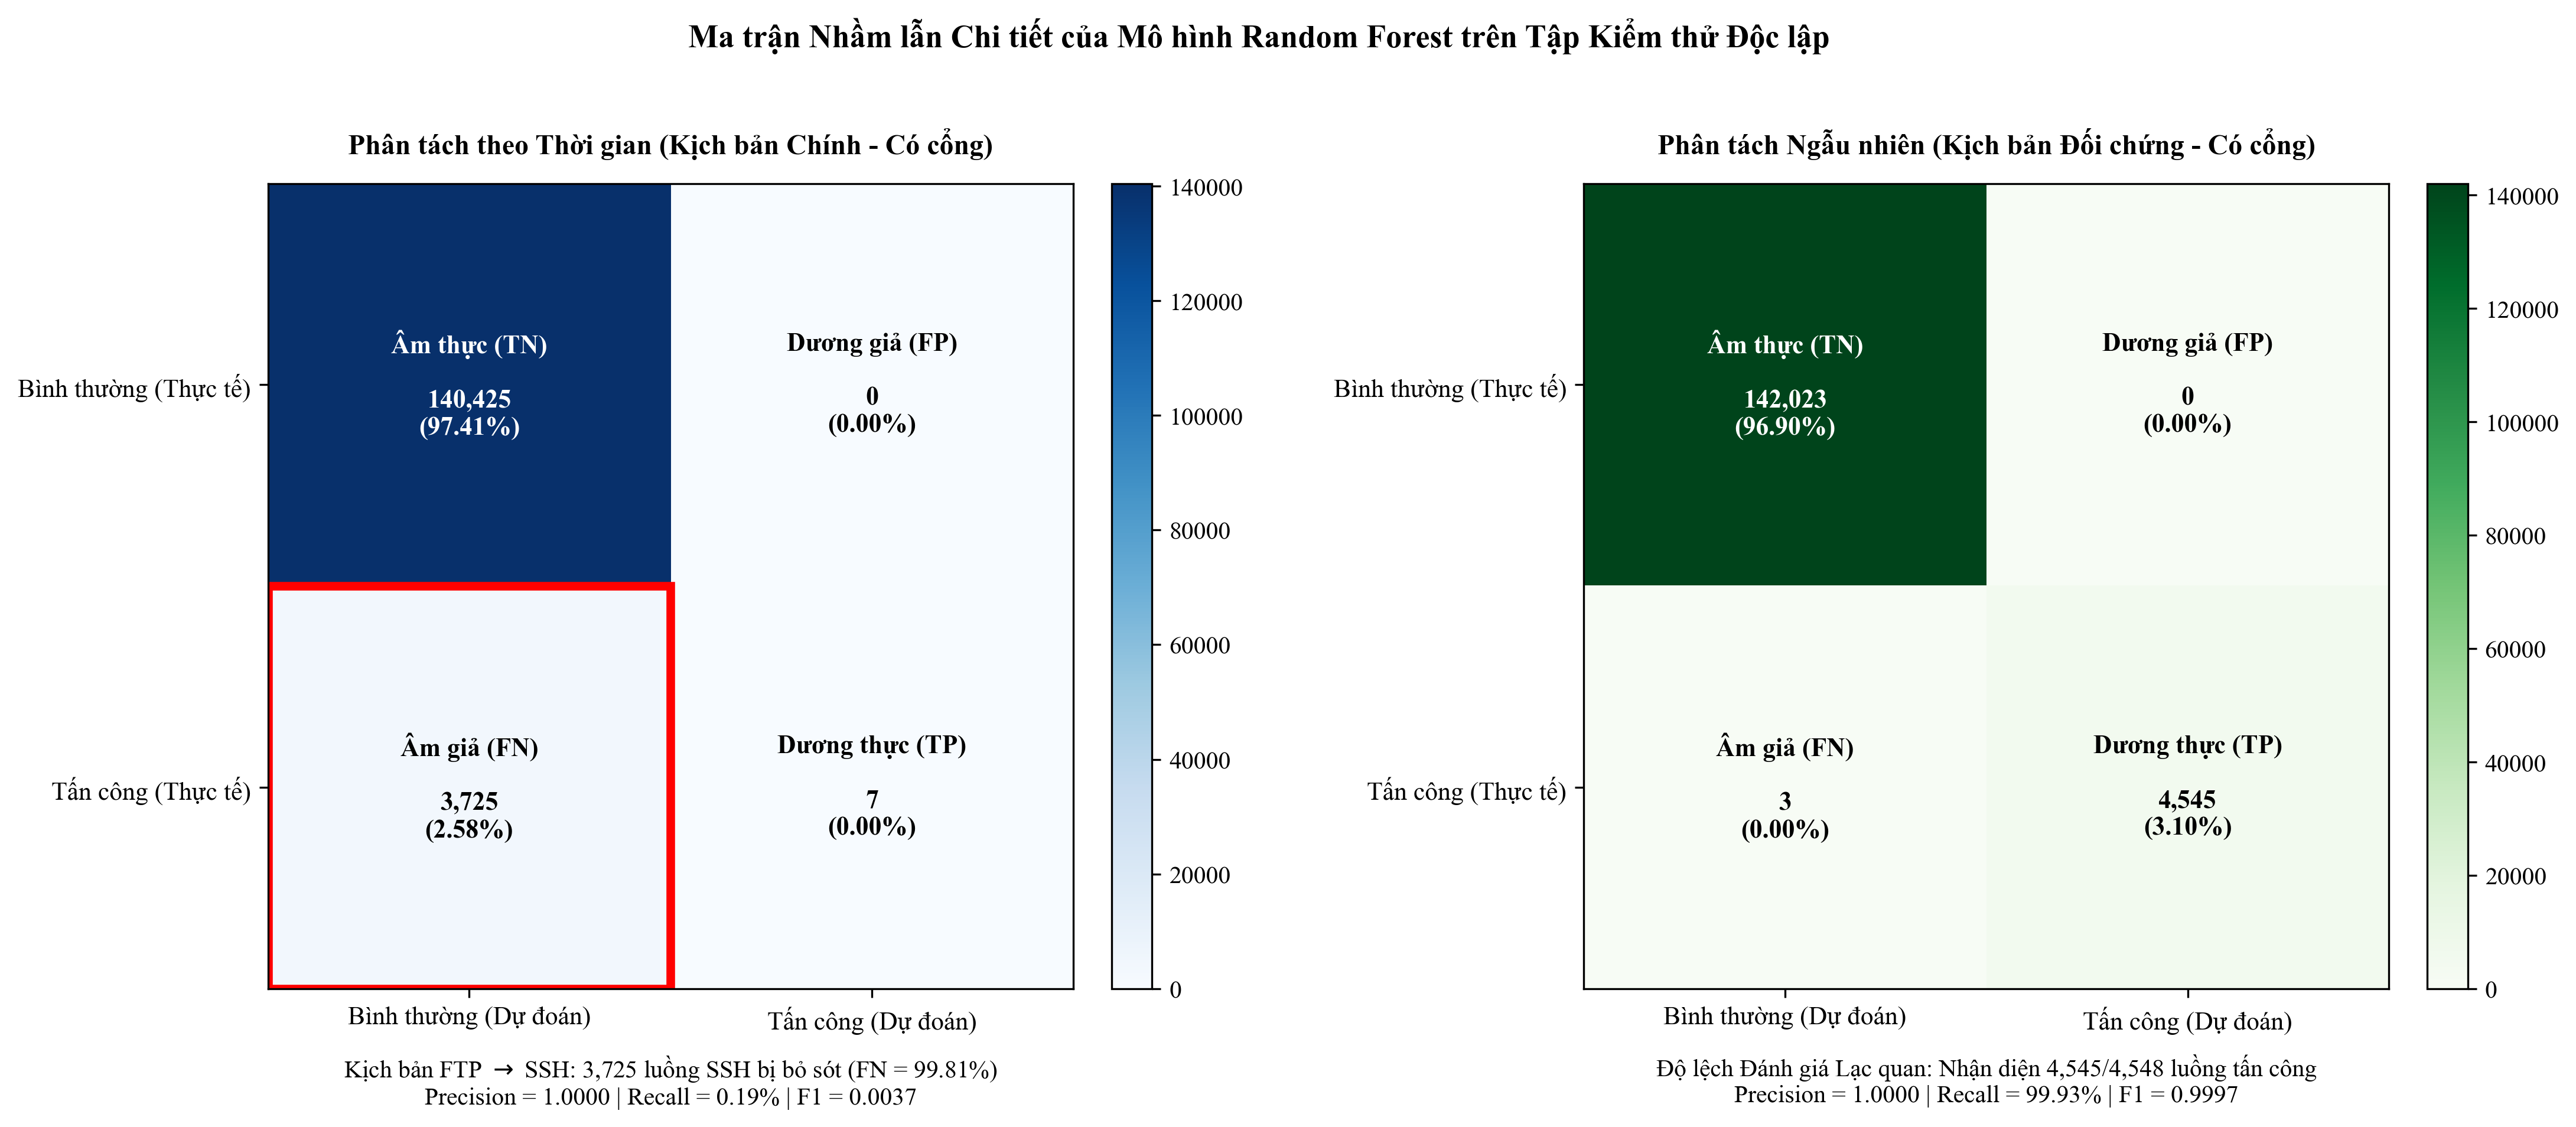
\includegraphics[width=0.92\textwidth]{experiments/figures/03_confusion_matrices_detailed.png}
\caption{Ma trận nhầm lẫn chi tiết của các mô hình trên tập kiểm thử phân tách theo thời gian, thể hiện trực quan tỷ lệ True Positive rất thấp đối với biến thể tấn công SSH.}
\label{fig:confusion_matrices_detailed}
\end{figure}

\noindent\textbf{Ghi nhận về Support và FTP Recall trên tập Test:}
Do tập $\Dtest$ theo thời gian diễn ra từ 14:32 đến 17:00 chiều (chỉ xuất hiện chiến dịch \SSH), số lượng mẫu hỗ trợ của \FTP\ là $0$ ($\text{FTP Support} = 0$). Theo đúng nguyên tắc trung thực học thuật đã đề ra, chỉ số FTP Recall trên tập Test được ghi nhận là N/A (Not Applicable), không gán giá trị 0\% hay 100\%.

\noindent\textbf{Nhận xét kết quả:}
Trong kịch bản đánh giá chính theo thời gian có cổng, Random Forest đạt $\FOne = \RFTestFOne$ với $\text{SSH Recall} = \RFTestSSHRecall$ (\RFTestTP/\DataTestSSH\ flow SSH), trong khi Decision Tree và XGBoost có $\FOne = \DTTestFOne$. Kết quả cho thấy các mô hình học máy dạng cây gặp khó khăn khi áp dụng lên subtype SSH không có trong tập fit của benchmark chuẩn. Tuy nhiên, \DataValidationSSH\ mẫu SSH trong Validation và nhãn của chúng tham gia lựa chọn siêu tham số; vì vậy đây là đánh giá subtype vắng mặt trong tập fit, không phải phép thử zero-shot khép kín từ đầu đến cuối.

% ==============================================================================
% reports/sections/results/06_04_random_control.tex
% ==============================================================================

\section{Kết quả thực nghiệm trên Random Split}

Trong Random Split có cổng, các mô hình đạt F1 cao trên tập kiểm thử (xem Phần B của Bảng \ref{tab:test_comparison}). Kết quả này được so sánh với Time-based Split ở phần sau; hai giao thức khác nhau cả về cách phân tách lẫn thành phần subtype:
\begin{itemize}
    \item Decision Tree: Đạt $\FOne = \DTRandomFOne$, $\Precision = \DTRandomPrecision$, $\Recall = \DTRandomRecall$, $\AP = \DTRandomAP$, $\ROCAUC = \DTRandomROCAUC$. Tỷ lệ phát hiện đạt \DTRandomFTPRecall\ đối với FTP và \DTRandomSSHRecall\ đối với SSH.
    \item Random Forest: Đạt $\FOne = \RFRandomFOne$, $\Precision = \RFRandomPrecision$, $\Recall = \RFRandomRecall$, $\AP = \RFRandomAP$, $\ROCAUC = \RFRandomROCAUC$. Tỷ lệ phát hiện đạt \RFRandomFTPRecall\ đối với FTP và \RFRandomSSHRecall\ đối với SSH.
    \item XGBoost:
    Đạt $\FOne = \XGBRandomFOne$, $\Precision = \XGBRandomPrecision$, $\Recall = \XGBRandomRecall$, $\AP = \XGBRandomAP$, $\ROCAUC = \XGBRandomROCAUC$. Tỷ lệ phát hiện đạt \XGBRandomFTPRecall\ đối với FTP và \XGBRandomSSHRecall\ đối với SSH.
\end{itemize}

\subsection{Đối chiếu kết quả giữa hai giao thức}
Bảng \ref{tab:split_diff} trình bày F1 và chênh lệch giữa hai giao thức phân tách trên tập Validation. Đây là phép đối chiếu tổng thể, không cô lập riêng tác động của chiến lược chia.

\begin{table}[htbp]
\centering
\caption{Chênh lệch F1 ($\Delta\text{F1}$) giữa Random Split và Time-based Split trên tập Validation.}
\label{tab:split_diff}
\adjustbox{max width=\textwidth}{%
\begin{tabular}{llrrrr}
\toprule
\textbf{Mô hình} & \textbf{Kịch bản cổng} & \textbf{F1 (Time-based Split)} & \textbf{F1 (Random Split)} & \textbf{$\Delta\text{F1}$} & \textbf{SSH Recall (Random)} \\
\midrule
Decision Tree & Có cổng & 0.7170 & 0.9939 & 0.2769 & 99.53\% \\
Decision Tree & Không cổng & 0.7169 & 0.9799 & 0.2631 & 98.87\% \\
Random Forest & Có cổng & 0.7181 & 0.9997 & 0.2816 & 99.89\% \\
Random Forest & Không cổng & 0.7134 & 0.9942 & 0.2808 & 99.05\% \\
XGBoost & Có cổng & 0.7181 & 0.9995 & 0.2814 & 100.00\% \\
XGBoost & Không cổng & 0.7136 & 0.9984 & 0.2848 & 99.67\% \\
\bottomrule
\end{tabular}%
}
\end{table}


Khoảng cách chênh lệch hiệu năng ($\Delta\FOne$) giữa Random Split và Time-based Split trên tập Validation dao động từ 0.2631 đến 0.2848. Trên tập Test, Random Forest đạt F1 lần lượt là \RFTestFOne\ và \RFRandomFOne\ trong hai giao thức. Tuy nhiên, thành phần subtype cũng khác nhau: Time-based Test chỉ có SSH, còn Random Test có SSH và FTP; Train của Random Split cũng đã có mẫu SSH, trong khi Train của Time-based Split không có SSH. Vì thế, chênh lệch không thể quy riêng cho thuật toán chia hoặc cho tương quan giữa các flow. Hình \ref{fig:data_leakage_benchmark} minh họa đối chiếu kết quả giữa hai giao thức.

\begin{figure}[htbp]
\centering
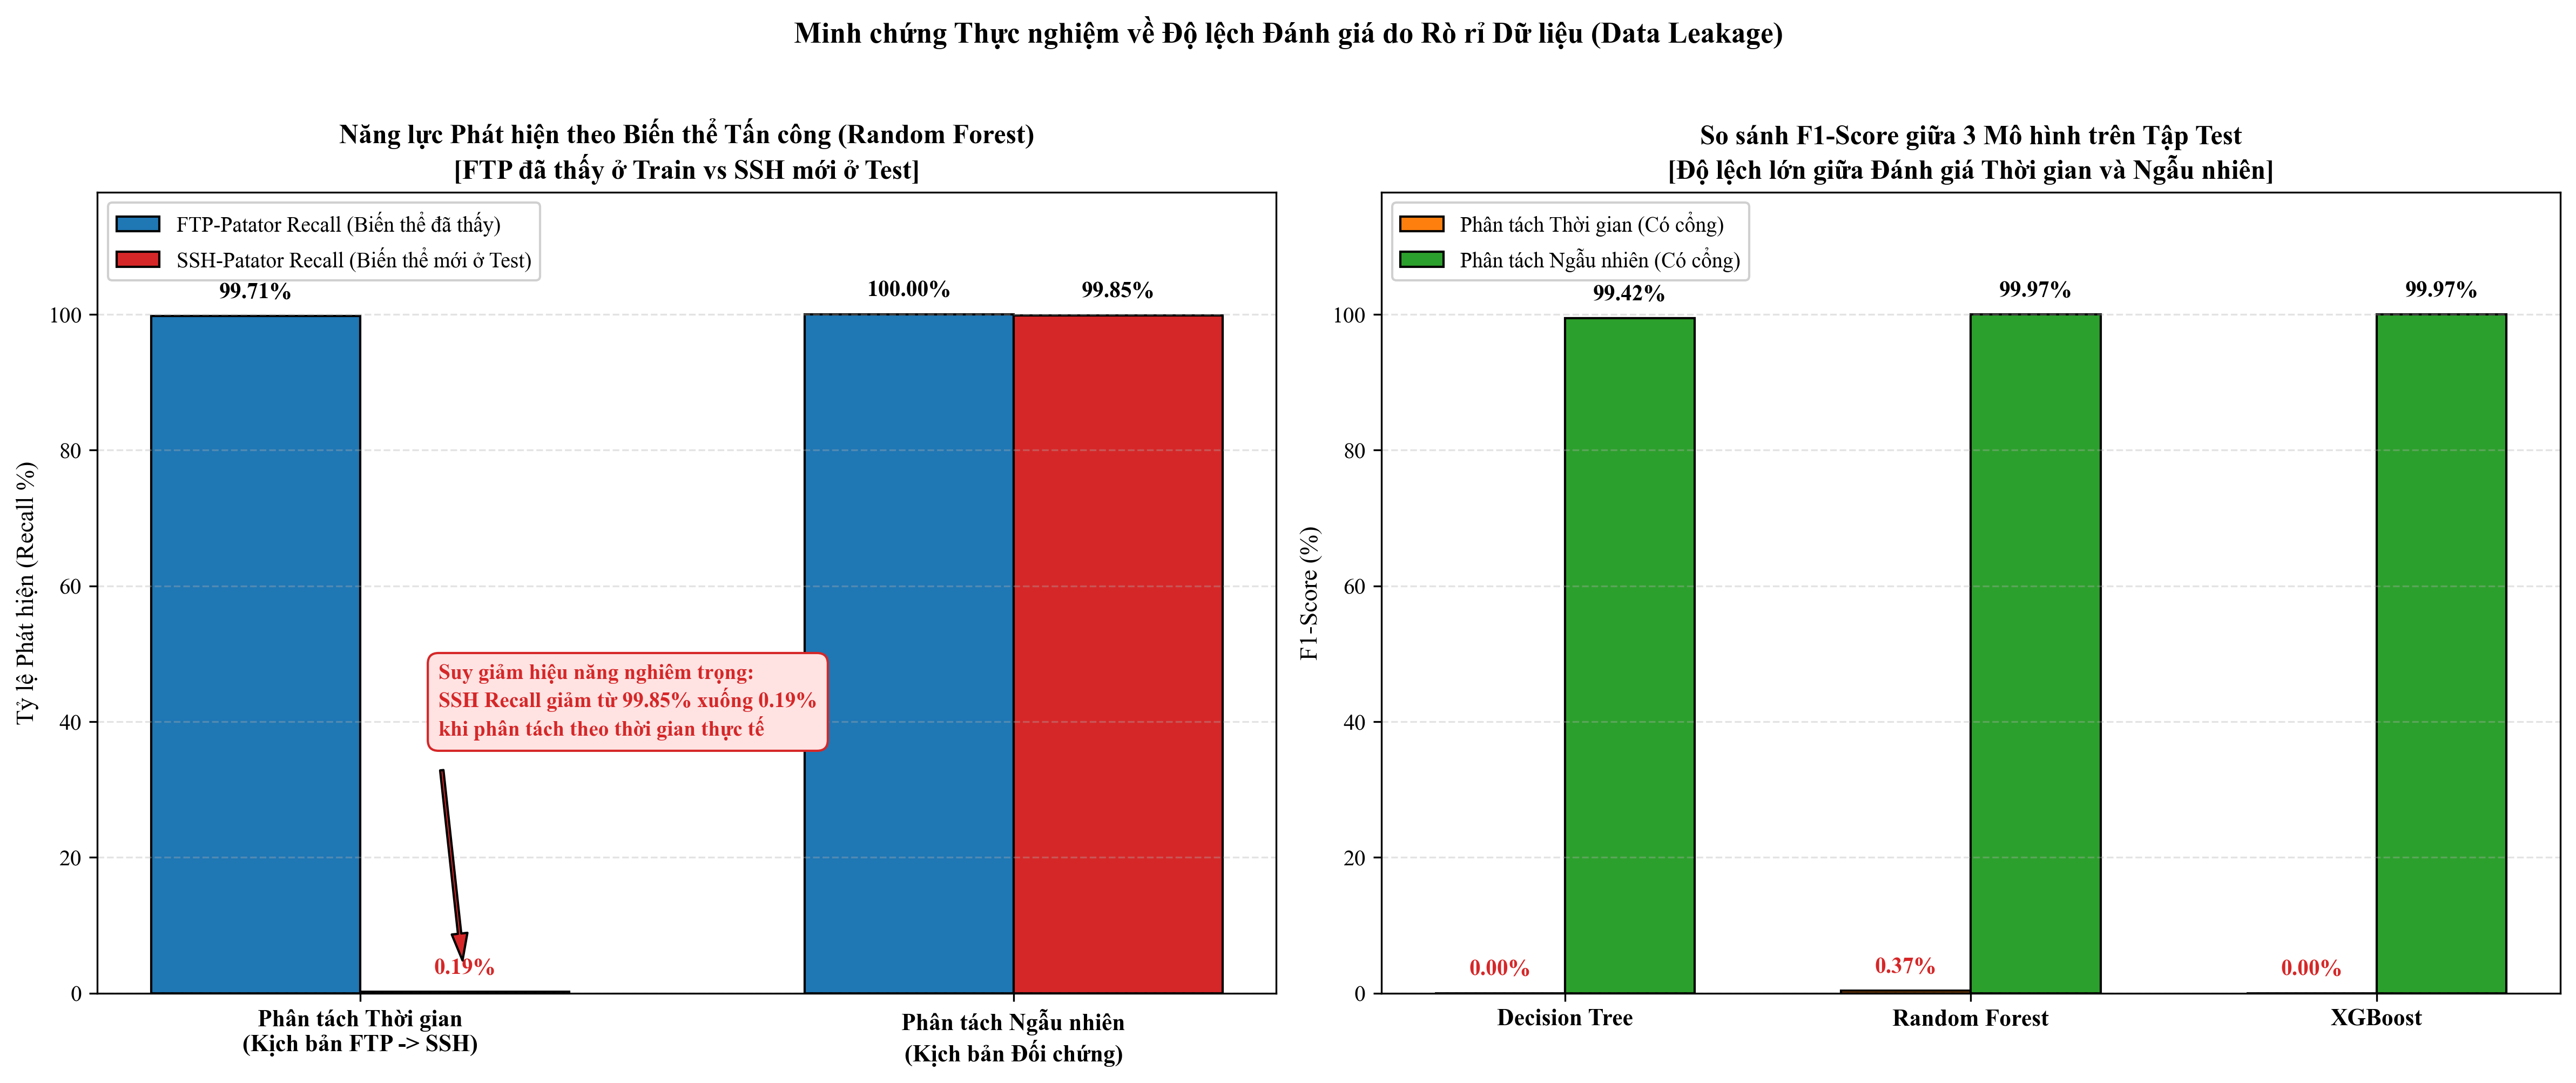
\includegraphics[width=0.92\textwidth]{experiments/figures/06_data_leakage_benchmark.png}
\caption{Đối chiếu hiệu năng giữa Random Split và Time-based Split; chênh lệch đồng thời phản ánh khác biệt về giao thức và thành phần subtype.}
\label{fig:data_leakage_benchmark}
\end{figure}

Kết quả này phù hợp với các phân tích của Arp và cộng sự \cite{arp2022dos} cũng như Pendlebury và cộng sự \cite{pendlebury2019tesseract}, theo đó chia ngẫu nhiên có thể tạo ra ước lượng lạc quan khi các mẫu phụ thuộc hoặc thuộc cùng chiến dịch xuất hiện ở nhiều tập. Trong thí nghiệm này, campaign-level dependence là một giải thích khả dĩ, nhưng chưa có bằng chứng trực tiếp về rò rỉ nhãn hay đặc trưng. Điểm số cao của Random Split không nên được diễn giải riêng như bằng chứng về khái quát hóa sang chiến dịch, subtype hoặc thời điểm mới; muốn cô lập tác động của chiến lược chia cần kiểm soát thành phần subtype và phân bố Test tương đương.

% ==============================================================================
% reports/sections/results/06_05_port_ablation.tex
% ==============================================================================

\section{Kết quả thực nghiệm bóc tách cổng mạng}

Để kiểm chứng giả thuyết cho rằng mô hình gặp khó khăn trên tập Test theo thời gian chỉ đơn thuần là do dựa vào lối tắt cổng dịch vụ đích (\texttt{Destination Port}), nhóm tiến hành phân tích kịch bản bóc tách cổng (\texttt{without\_port}), trong đó đặc trưng này bị loại bỏ khỏi không gian huấn luyện.

Bảng \ref{tab:port_ablation} tổng hợp kết quả bóc tách cổng trên tập kiểm định $\Dval$.

% ==============================================================================
% reports/tables/generated/tab_port_ablation.tex
% ==============================================================================
\begin{table}[htbp]
\centering
\caption{Thực nghiệm Bóc tách Cổng mạng (Port Ablation) trên tập Validation phân tách theo thời gian.}
\label{tab:port_ablation}
\resizebox{\textwidth}{!}{%
\begin{tabular}{lrrrrr}
\toprule
\textbf{Mô hình} & \textbf{\FOne\ (Có Cổng)} & \textbf{\FOne\ (Không Cổng)} & \textbf{$\Delta$\FOne} & \textbf{SSH Recall (Có)} & \textbf{SSH Recall (Không)} \\
\midrule
Decision Tree & 0.7170 & 0.7169 & 0.0001 & 0.00\% & 0.00\% \\
Random Forest & 0.7181 & 0.7134 & 0.0047 & 0.00\% & 0.00\% \\
XGBoost & 0.7181 & 0.7136 & 0.0045 & 0.00\% & 0.00\% \\
\bottomrule
\end{tabular}%
}
\end{table}


Trên tập kiểm định $\Dval$, việc loại bỏ cổng làm giảm nhẹ điểm F1 của cả 3 mô hình (khoảng 0.0001 đến 0.0047), và tỷ lệ phát hiện tấn công SSH vẫn giữ ở mức 0.00\% (do mô hình tối ưu theo mẫu FTP chiếm đa số trong tập Val).

Khi quan sát kết quả trên tập kiểm thử $\Dtest$ theo thời gian (xem lại Phần A của Bảng \ref{tab:test_comparison}):
\begin{itemize}
    \item \textbf{Cây Quyết Định (Decision Tree)}: Điểm F1 tăng nhẹ từ 0.0000 lên \textbf{\DTTestWithoutPortFOne}, nhận diện được \DTTestWithoutPortSSHRecall\ tấn công SSH (7 mẫu).
    \item \textbf{Rừng Ngẫu Nhiên (Random Forest)}: Điểm F1 tăng từ \RFTestFOne\ lên \textbf{\RFTestWithoutPortFOne}, nhận diện được \RFTestWithoutPortSSHRecall\ tấn công SSH (14 trên tổng số 3,732 mẫu).
    \item \textbf{XGBoost}: Điểm F1 tăng từ 0.0000 lên \textbf{\XGBTestWithoutPortFOne}, nhận diện được \XGBTestWithoutPortSSHRecall\ tấn công SSH (13 trên tổng số 3,732 mẫu).
\end{itemize}

Sự thay đổi diện tích dưới đường cong ROC và đường cong Precision-Recall giữa hai kịch bản có và không có cổng được đối chiếu trực quan trên Hình \ref{fig:roc_pr_comparative}.

\begin{figure}[htbp]
\centering
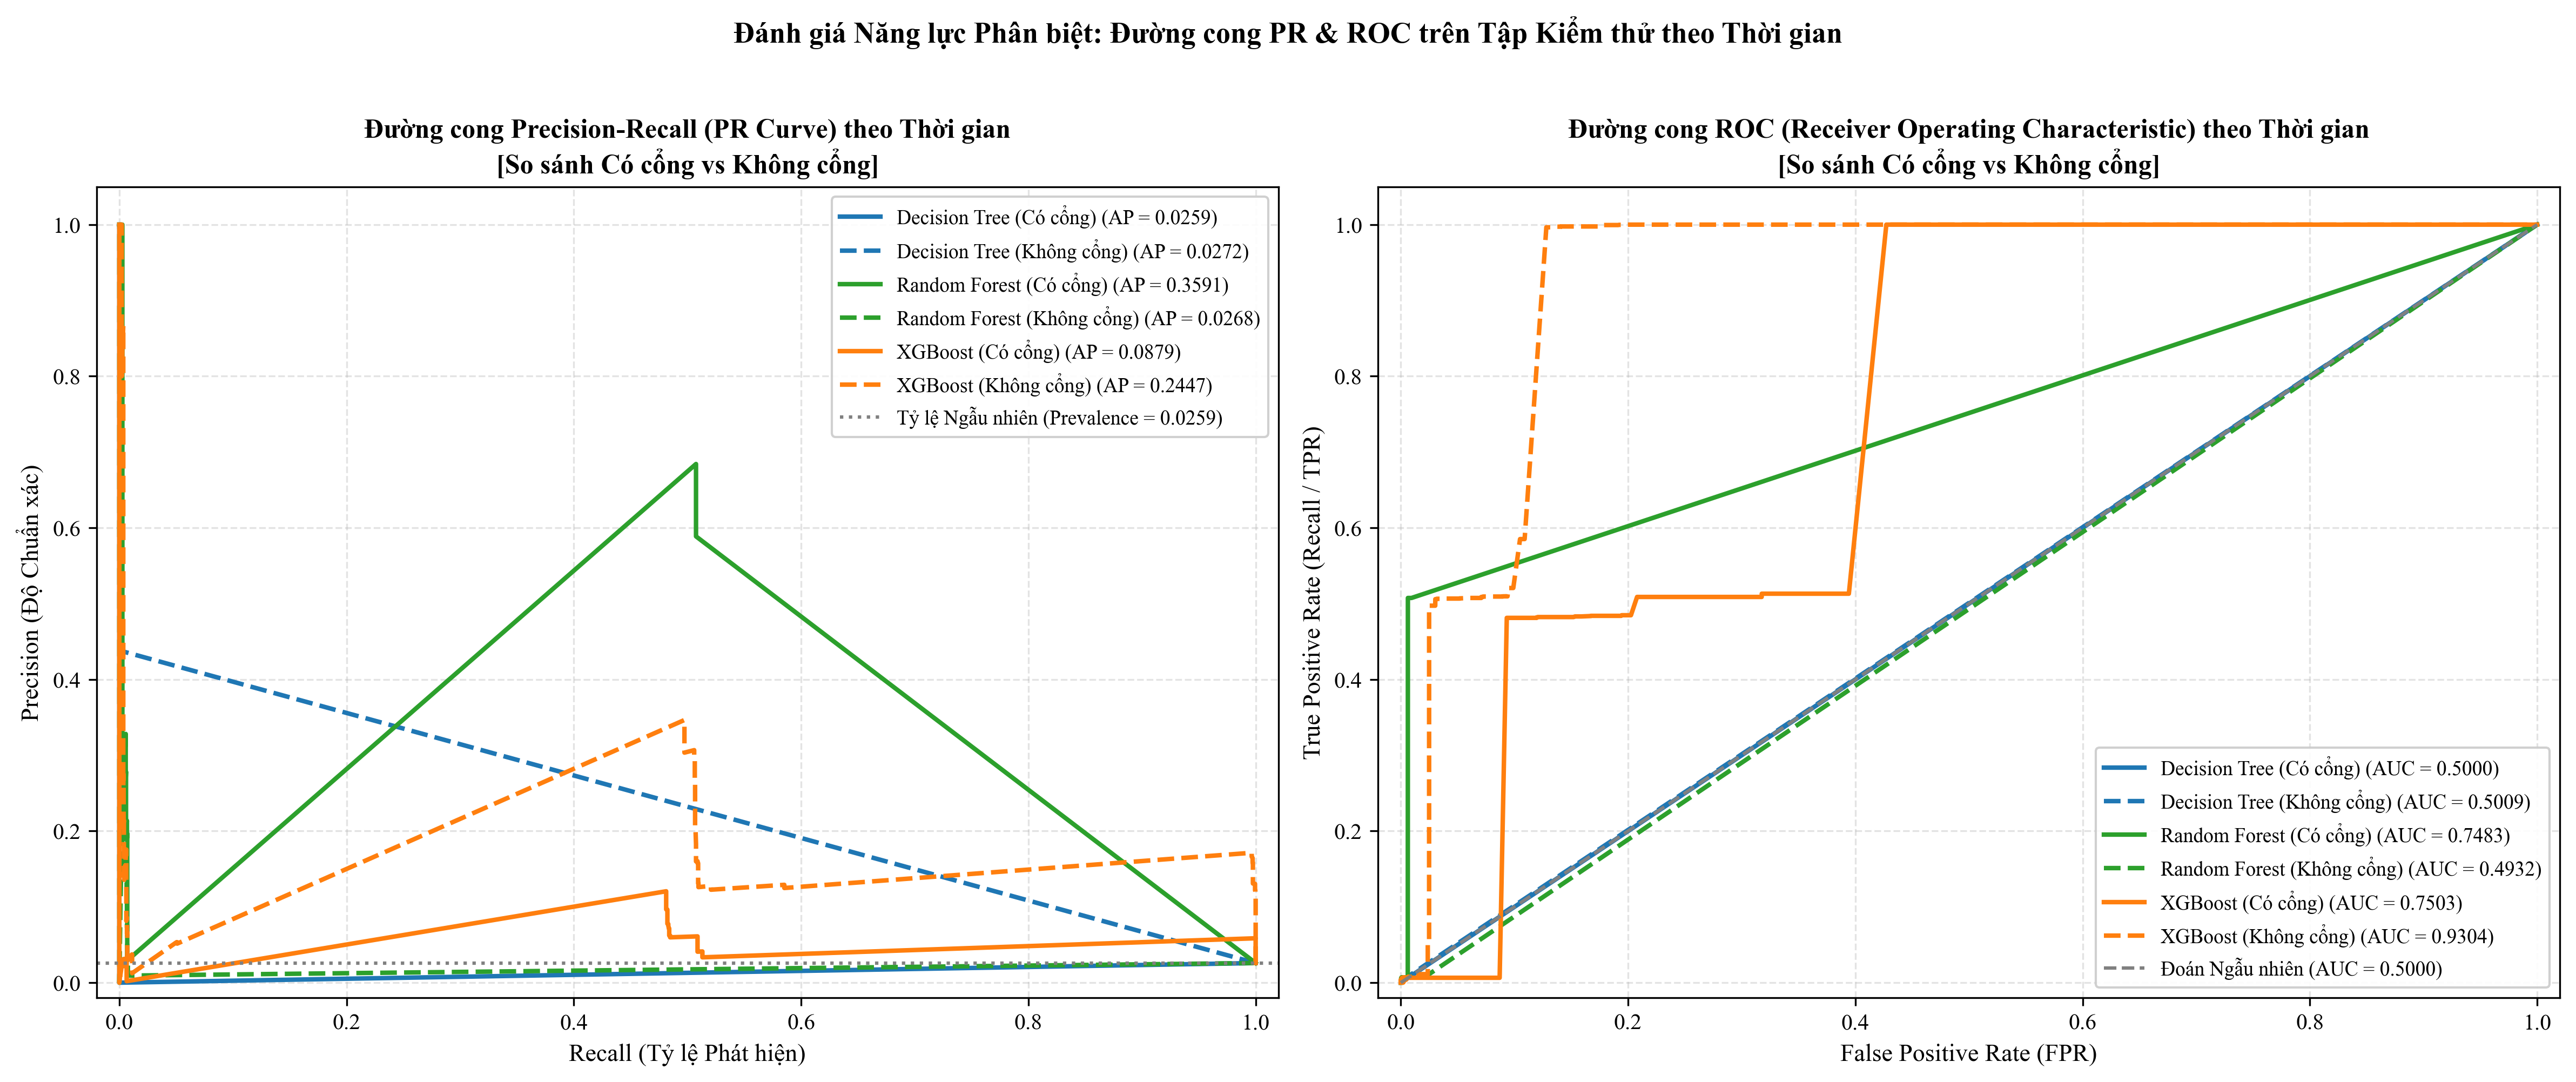
\includegraphics[width=0.92\textwidth]{experiments/figures/04_roc_and_pr_curves_comparative.png}
\caption{Đường cong ROC và Precision-Recall đối chiếu giữa các mô hình và kịch bản thực nghiệm, phản ánh sự biến thiên diện tích dưới đường cong khi có và không có đặc trưng cổng mạng.}
\label{fig:roc_pr_comparative}
\end{figure}

\noindent\textbf{Kết luận về vai trò của cổng dịch vụ:}
Việc loại bỏ cổng dịch vụ giúp các mô hình nhận diện được thêm một lượng nhỏ các flow SSH dựa trên đặc trưng hành vi (tỷ lệ SSH Recall tăng từ $0.00\% \text{ -- } 0.19\%$ lên $0.19\% \text{ -- } 0.38\%$).

Tuy nhiên, hiệu năng tổng thể của mô hình trong toàn bộ các tổ hợp theo thời gian vẫn ở mức rất thấp, với giá trị F1 cao nhất được ghi nhận là \textbf{\RFTestWithoutPortFOne} ở Random Forest (nhận diện được \RFTestWithoutPortSSHRecall\ tấn công SSH, tức 14/3,732 flow). Kết quả này cho thấy: mặc dù \texttt{Destination Port} là một lối tắt quan trọng của mô hình, việc loại bỏ cổng không đủ để giải quyết sự suy giảm hiệu năng tổng quát hóa. Nói cách khác, sự sụt giảm hiệu năng trong việc phát hiện SSH không thể được giải thích chỉ bằng riêng yếu tố cổng dịch vụ. Sự khác biệt về cơ chế hoạt động và phân phối đặc trưng thống kê gói tin giữa hai giao thức FTP và SSH (kết hợp với yếu tố thời gian và chiến dịch tấn công) là một cơ chế hợp lý góp phần tạo nên sự dịch chuyển phân phối này.

% ==============================================================================
% reports/sections/results/06_06_explainability.tex
% ==============================================================================

\section{Phân tích khả năng giải thích}

Để làm rõ hành vi dự đoán bên trong của mô hình trên tập mẫu kiểm định, nhóm áp dụng phương pháp giải thích gia tăng Shapley (\textbf{SHAP TreeExplainer} \cite{lundberg2017unified}) kết hợp với việc trích xuất cấu trúc logic của Cây Quyết Định.

\subsection{Phân tích tầm quan trọng đặc trưng bằng SHAP}
Phân tích SHAP được thực hiện trên 500 mẫu đại diện từ tập kiểm định $\Dval$ đối với mô hình Random Forest theo thời gian có cổng. Bảng \ref{tab:shap_top10} liệt kê 10 đặc trưng có giá trị đóng góp trung bình tuyệt đối ($\text{Mean } |\text{SHAP}|$) lớn nhất.

% ==============================================================================
% reports/tables/generated/tab_shap_top10.tex
% ==============================================================================
\begin{table}[htbp]
\centering
\caption{Top 10 đặc trưng mạng có mức độ đóng góp phân loại lớn nhất theo SHAP TreeExplainer trên tập Validation.}
\label{tab:shap_top10}
\resizebox{\textwidth}{!}{%
\begin{tabular}{rlrl}
\toprule
\textbf{Hạng} & \textbf{Tên đặc trưng mạng} & \textbf{Mean $|$SHAP$|$} & \textbf{Ý nghĩa giao thức / thống kê mạng} \\
\midrule
1 & \texttt{Destination Port} & \SHAPTopOneVal & Cổng đích dịch vụ (Port 21 FTP, Port 22 SSH) \\
2 & \texttt{Fwd Packet Length Std} & \SHAPTopTwoVal & Độ lệch chuẩn kích thước gói tin hướng đi (Fwd) \\
3 & \texttt{Avg Fwd Segment Size} & 0.0292 & Kích thước phân đoạn trung bình hướng đi \\
4 & \texttt{Max Packet Length} & 0.0289 & Độ dài gói tin lớn nhất quan sát được trong flow \\
5 & \texttt{Packet Length Mean} & 0.0275 & Độ dài gói tin trung bình của toàn flow \\
6 & \texttt{min\_seg\_size\_forward} & 0.0272 & Kích thước header TCP tối thiểu phía forward \\
7 & \texttt{Packet Length Std} & 0.0271 & Độ lệch chuẩn độ dài toàn bộ gói tin trong flow \\
8 & \texttt{Fwd Packet Length Mean} & 0.0271 & Độ dài gói tin trung bình hướng đi (Fwd) \\
9 & \texttt{Average Packet Size} & 0.0262 & Kích thước gói tin trung bình tổng thể \\
10 & \texttt{Packet Length Variance} & 0.0208 & Phương sai phân bố độ dài gói tin trong flow \\
\bottomrule
\end{tabular}%
}
\end{table}


Kết quả định lượng cho thấy:
\begin{itemize}
    \item Đặc trưng \textbf{\texttt{Destination Port}} có giá trị lớn nhất với $\text{Mean } |\text{SHAP}| = \textbf{\SHAPTopOneVal}$.
    \item Đặc trưng xếp thứ hai là \texttt{Fwd Packet Length Std} đạt giá trị \textbf{\SHAPTopTwoVal}.
    \item Tỷ số đóng góp giữa đặc trưng số 1 và số 2 là xấp xỉ \textbf{\SHAPRatioTopOneTwo\ lần}.
\end{itemize}

Kết quả phân tích SHAP cho thấy mô hình phụ thuộc mạnh vào \texttt{Destination Port} trong kịch bản có cổng được phân tích, tận dụng cổng dịch vụ như một lối tắt phân loại quan trọng giữa lưu lượng bình thường và lưu lượng tấn công FTP (Cổng 21), như được minh họa trực quan trên biểu đồ phân bố giá trị SHAP (Hình \ref{fig:shap_summary}).

\begin{figure}[htbp]
\centering
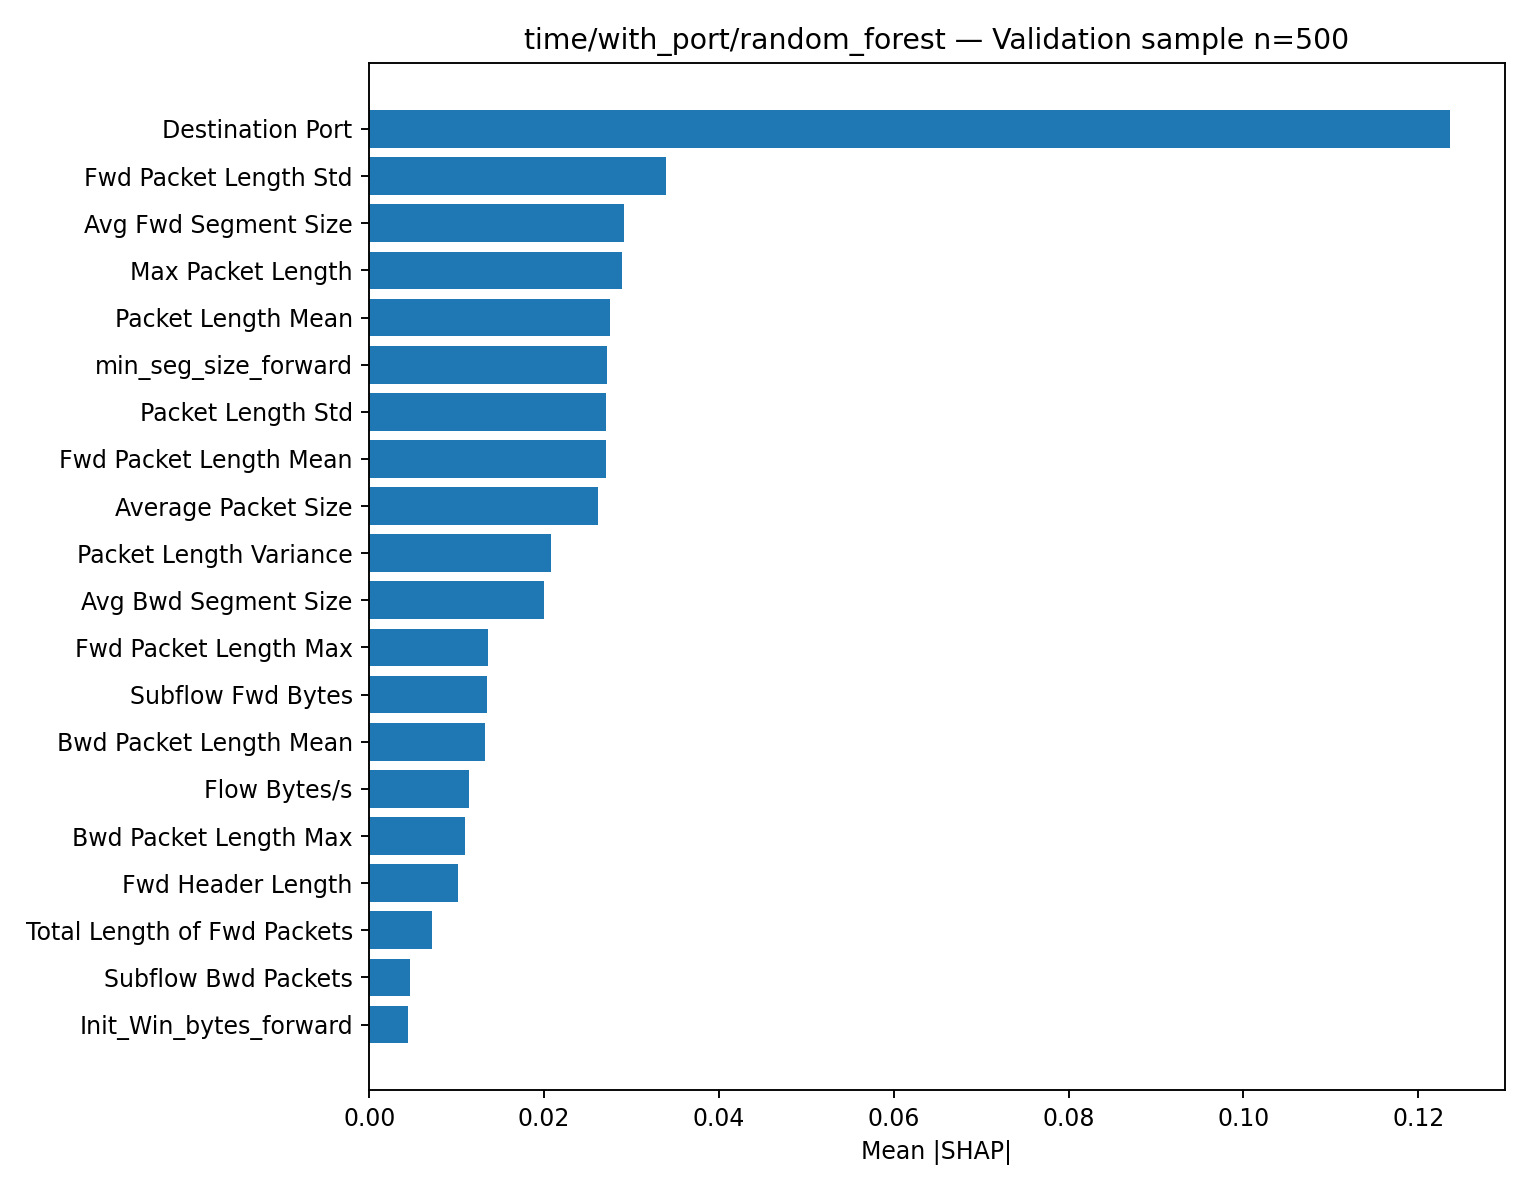
\includegraphics[width=0.85\textwidth]{artifacts/week3_week4/shap/summary.png}
\caption{Biểu đồ phân bố giá trị SHAP (SHAP Summary Plot) của Top các đặc trưng quan trọng trên 500 mẫu kiểm định.}
\label{fig:shap_summary}
\end{figure}

\subsection{Trích xuất cấu trúc cây quyết định}
\label{sec:tree_structure_analysis}
Quan sát cấu trúc logic của Cây Quyết Định càng làm sáng tỏ cơ chế phân nhánh này:
\begin{itemize}
    \item \textbf{Kịch bản có cổng:} Nút gốc (Root Node) phân chia dựa trên điều kiện \texttt{Destination Port <= 21.5} (Hình \ref{fig:tree_structure}). Các nhánh tiếp theo tiếp tục cô lập các flow có \texttt{Destination Port <= 20.5} (loại bỏ traffic cổng thấp) để định vị chính xác \textbf{Cổng 21 (FTP)}.
    \item \textbf{Kịch bản không có cổng:} Khi đặc trưng cổng bị loại bỏ, cây quyết định chọn nút gốc là \texttt{Average Packet Size <= 14.12} (chi tiết quy tắc văn bản trình bày tại Phụ lục \ref{app:tree_rules}).
\end{itemize}

\begin{figure}[htbp]
\centering
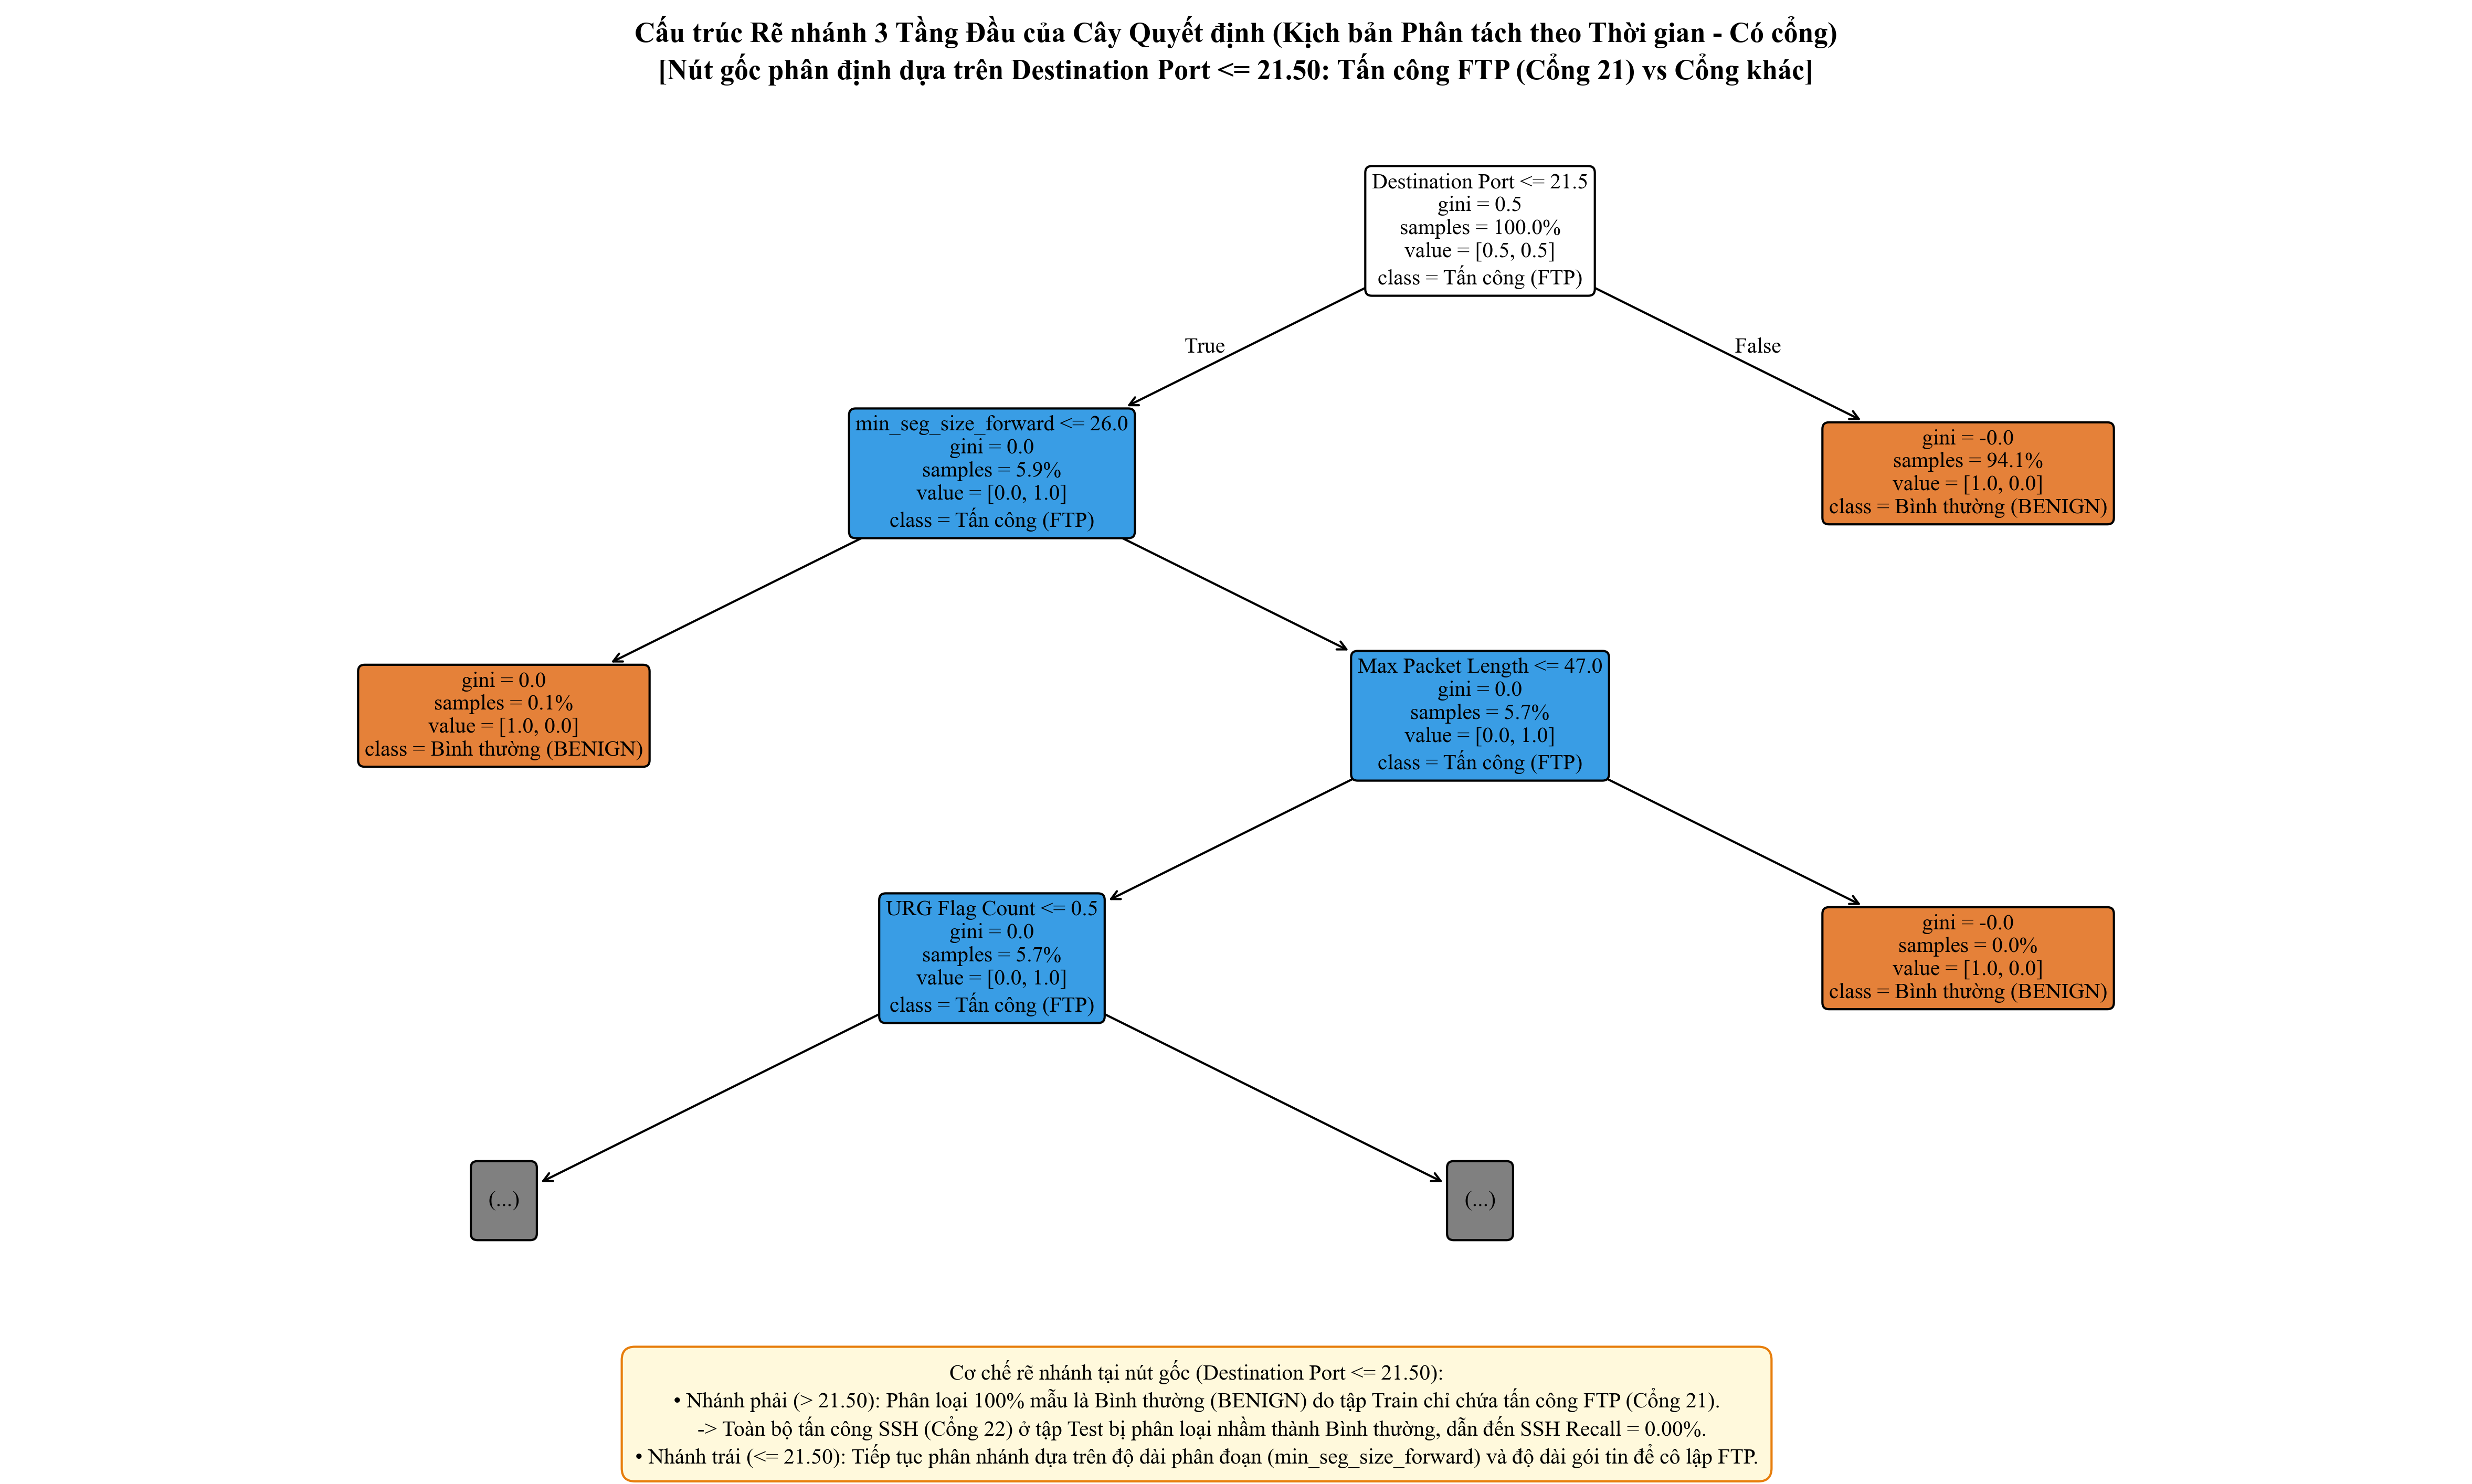
\includegraphics[width=0.95\textwidth]{experiments/figures/01_tree_structure_detailed.png}
\caption{Cấu trúc 3 tầng đầu tiên của Cây Quyết Định minh họa ngưỡng rẽ nhánh ưu tiên tại \texttt{Destination Port $\le$ 21.5}.}
\label{fig:tree_structure}
\end{figure}

Khi chuyển sang tập kiểm thử $\Dtest$, toàn bộ các cuộc tấn công đều diễn ra trên \textbf{Cổng 22 (SSH)}, tức là rơi vào nhánh \texttt{Destination Port > 21.5}. Tại nhánh này, vì trong tập Train mô hình chưa từng thấy cuộc tấn công nào diễn ra trên cổng $> 21$, phần lớn các nút lá tương ứng đều được gán nhãn là lưu lượng bình thường (\Normal, 0). Cấu trúc nhánh rẽ này giải thích vì sao cây quyết định không phát hiện được các flow SSH ở Cổng 22 trong kịch bản có cổng. Cần nhấn mạnh rằng SHAP và cấu trúc cây giải thích hành vi phân loại của mô hình trên tập mẫu quan sát, chứ không chứng minh quan hệ nhân quả trong môi trường mạng thực tế.

% ==============================================================================
% reports/sections/results/06_07_xgboost_refit_study.tex
% ==============================================================================

\section{Nghiên cứu điển hình: Tác động của thiết kế pipeline và cờ refit trên XGBoost}
\label{sec:results_refit}

Trong quá trình đối soát thực nghiệm giữa các đường ống trong mã nguồn, nhóm phát hiện sự phân kỳ số liệu đáng chú ý đối với thuật toán XGBoost:
\begin{itemize}
    \item Trong benchmark chuẩn mực tại \path{artifacts/week3_week4/test_comparison.csv}, XGBoost đạt $\FOne = \textbf{0.0000}$ ($\text{SSH Recall} = 0.00\%$).
    \item Trong kết quả tuning độc lập tại \path{experiments/w3_05_time_tuning/test_eval/test_metrics.json}, XGBoost lại đạt $\FOne = \textbf{\XGBRefitTestFOne}$ ($\text{SSH Recall} = \textbf{\XGBRefitTestSSHRecall}$).
\end{itemize}

\subsection{Truy vết nguyên nhân kỹ thuật trong mã nguồn}
Tiến hành phân tích mã nguồn \path{src/ids/tune_xgboost.py}, nguyên nhân kỹ thuật được xác định tại dòng 151--168:
\begin{lstlisting}[language=Python, caption={Đoạn mã cấu hình RandomizedSearchCV và gộp dữ liệu gây kích hoạt refit trên tập gộp.}]
search = RandomizedSearchCV(
    estimator=base_model,
    param_distributions=param_distributions,
    n_iter=n_iter,
    scoring=f1_scorer,
    cv=cv_split, # Phân tách tùy biến giữa Train và Validation
    # refit=True là giá trị mặc định của scikit-learn
)
X_combined = pd.concat([X_train, X_val], axis=0).reset_index(drop=True)
y_combined = pd.concat([y_train, y_val], axis=0).reset_index(drop=True)
search.fit(X_combined, y_combined)
joblib.dump(search.best_estimator_, best_model_path)
\end{lstlisting}

Theo tài liệu đặc tả của thư viện \texttt{scikit-learn} \cite{scikit_learn_refit}, tham số \texttt{refit} có giá trị mặc định là \texttt{True}. Sau khi hoàn tất việc đánh giá các tổ hợp siêu tham số trên \texttt{cv\_split} (sử dụng tập con Train làm fold huấn luyện và Val làm fold kiểm định), đối tượng \texttt{RandomizedSearchCV} hoạt động đúng theo đặc tả: gọi hàm \texttt{fit()} của mô hình tốt nhất trên toàn bộ tập dữ liệu đầu vào đã truyền vào hàm \texttt{fit()}, tức là toàn bộ tập gộp $\mathbf{X}_{\text{combined}} = \Xtrain \cup \Xval$.

Lỗi ở đây nằm ở thiết kế đường ống: dữ liệu Train và Validation được chủ động gộp trước khi truyền vào \texttt{RandomizedSearchCV.fit()}, trong khi \texttt{refit=True} khiến mô hình tốt nhất được huấn luyện lại trên toàn bộ tập gộp đó.

\subsection{Hậu quả đối với bản chất bài toán đánh giá}
Trong khi tập $\Dtrain$ không chứa mẫu \SSH\ nào (0 flow), thì tập kiểm định $\Dval$ lại chứa \textbf{1,886 flow tấn công \SSH}.

Khi cơ chế \texttt{refit=True} diễn ra trên tập dữ liệu gộp:
\begin{enumerate}
    \item Mô hình XGBoost được huấn luyện trực tiếp trên 1,886 mẫu tấn công SSH từ tập Validation.
    \item Bài toán đánh giá trên tập Test theo thời gian đã bị biến đổi bản chất từ \textbf{kịch bản tổng quát hóa FTP $\to$ SSH (không có SSH trong tập huấn luyện)} thành \textbf{học có giám sát trên biến thể đã biết (\textit{Seen-Subtype Supervised Learning}) do được huấn luyện trên 1,886 mẫu SSH}.
    \item Việc được học trên 1,886 mẫu SSH này đã giúp XGBoost tiếp thu phân phối đặc trưng và cổng 22 của SSH, làm cho điểm số trên tập Test tăng từ \textbf{0.0000 lên \XGBRefitTestFOne}.
\end{enumerate}

Bảng \ref{tab:refit_comparison} tổng hợp sự đối lập giữa hai chế độ đánh giá này.

\begin{table}[htbp]
\centering
\caption{Đối chiếu hiệu năng của XGBoost giữa chế độ đánh giá tổng quát hóa chuẩn mực và chế độ tiếp xúc validation do thiết kế pipeline (Refit).}
\label{tab:refit_comparison}
\adjustbox{max width=\textwidth}{%
\begin{tabular}{lllrr}
\toprule
\textbf{Chế độ thực nghiệm} & \textbf{Dữ liệu thực tế fit mô hình} & \textbf{Mẫu SSH trong tập fit} & \textbf{Test F1-Score} & \textbf{Test SSH Recall} \\
\midrule
Chế độ 1: Tổng quát hóa chuẩn mực & Duy nhất Train ($\Dtrain$) & \DataTrainSSH\ mẫu & \textbf{\XGBTestFOne} & \textbf{\XGBTestSSHRecall} \\
Chế độ 2: Pipeline gộp tập (Refit) & Train + Val ($\Dtrain \cup \Dval$) & \DataValidationSSH\ mẫu & \textbf{\XGBRefitTestFOne} & \textbf{\XGBRefitTestSSHRecall} \\
\bottomrule
\end{tabular}%
}
\end{table}

Phát hiện này mang lại một bài học thực hành giá trị trong kỹ nghệ MLOps: việc chủ động gộp Train và Validation trước khi gọi hàm tìm kiếm siêu tham số kết hợp với hành vi mặc định \texttt{refit=True} của thư viện có thể làm thay đổi bản chất bài toán đánh giá nếu không được kiểm soát ranh giới dữ liệu một cách cẩn trọng.


% ==============================================================================
% reports/chapters/07_ket_luan.tex
% CHƯƠNG 7: KẾT LUẬN VÀ HƯỚNG PHÁT TRIỂN
% ==============================================================================

\chapter{Kết Luận và Hướng Phát Triển}
\label{chap:ket_luan}

Chương này tổng kết toàn bộ các kết quả đạt được từ quá trình nghiên cứu thực nghiệm, trả lời trực tiếp bốn câu hỏi nghiên cứu đã đặt ra, đồng thời phân tích các mối đe dọa đến tính hợp lệ, đề xuất các hướng mở rộng trong tương lai và báo cáo chi tiết bảng phân công nhiệm vụ của các thành viên trong nhóm.

\section{Tổng kết kết quả và trả lời các câu hỏi nghiên cứu}
\label{sec:rq_answers}

Thực nghiệm trên CICIDS2017 với 12 tổ hợp mô hình và kịch bản dữ liệu cho phép trả lời bốn câu hỏi nghiên cứu:

\begin{enumerate}
    \item \textbf{Câu hỏi nghiên cứu 1 (RQ1 -- Đánh giá trên subtype SSH vắng mặt trong tập fit theo thời gian):}\\
    Khi mô hình học máy dạng cây chỉ được huấn luyện trên tập Train chứa biến thể \FTP, khả năng phát hiện biến thể \SSH\ xuất hiện ở giai đoạn thời gian sau suy giảm nghiêm trọng. Trong kịch bản thực nghiệm chính có cổng mạng (\texttt{time/with\_port}), Random Forest chỉ đạt $\FOne = \RFTestFOne$ với $\text{SSH Recall} = \RFTestSSHRecall$ (chỉ nhận diện chính xác \RFTestTP\ trên tổng số \DataTestSSH\ luồng tấn công SSH), trong khi Decision Tree và XGBoost hoàn toàn không phát hiện được bất kỳ luồng SSH nào ($\FOne = \DTTestFOne$, $\text{SSH Recall} = \DTTestSSHRecall$). Mặc dù tập kiểm định có chứa \DataValidationSSH\ mẫu SSH tham gia vào quá trình lựa chọn siêu tham số, việc mô hình không được huấn luyện trên mẫu SSH nào trong tập Train vẫn khiến tỷ lệ phát hiện biến thể mới trên tập kiểm thử ở mức rất thấp.

    \item \textbf{Câu hỏi nghiên cứu 2 (RQ2 -- So sánh các giao thức phân tách):}\\
    Random Split và Time-based Split cho kết quả khác biệt. Trên tập kiểm thử, F1 của Random Forest lần lượt là $\RFRandomFOne$ và $\RFTestFOne$; tỷ lệ phát hiện SSH lần lượt là \RFRandomSSHRecall\ và \RFTestSSHRecall. Đây là so sánh giữa hai giao thức có thành phần subtype khác nhau: Train/Test của Random Split chứa SSH, Test còn có FTP; Time-based Train không có SSH và Test chỉ có SSH. Vì vậy, không thể quy toàn bộ chênh lệch cho cách chia hoặc cho tương quan giữa các flow. Sự phụ thuộc giữa các flow cùng chiến dịch có thể góp phần làm ước lượng Random Split lạc quan, nhưng nghiên cứu không xác lập trực tiếp rò rỉ nhãn hay đặc trưng.

    \item \textbf{Câu hỏi nghiên cứu 3 (RQ3 -- Vai trò của cổng dịch vụ và các đặc trưng hành vi):}\\
    \texttt{Destination Port} đóng vai trò là một lối tắt phân loại chi phối mạnh mẽ quyết định của mô hình. Phân tích SHAP chỉ ra cổng dịch vụ có giá trị đóng góp trung bình tuyệt đối $\text{Mean } |\text{SHAP}| = \SHAPTopOneVal$, gấp \SHAPRatioTopOneTwo\ lần đặc trưng xếp thứ hai. Khi loại bỏ cổng dịch vụ khỏi không gian huấn luyện (\texttt{without\_port}), mô hình nhận diện được thêm một lượng nhỏ các luồng SSH dựa trên hình thái thống kê gói tin (tỷ lệ SSH Recall tăng lên mức $\RFTestSSHRecall\ \text{--} \RFTestWithoutPortSSHRecall$), với F1 cao nhất đạt $\RFTestWithoutPortFOne$ ở Random Forest (14/\DataTestSSH\ luồng SSH). Tuy nhiên, hiệu năng tổng thể vẫn ở mức rất thấp, chứng minh rằng sự thất bại trong việc phát hiện SSH không thể được giải thích chỉ bằng riêng yếu tố cổng dịch vụ. Sự khác biệt về cơ chế hoạt động và phân phối đặc trưng hình thái gói tin giữa FTP và SSH, cùng với yếu tố thời gian, phù hợp với hiện tượng dịch chuyển phân phối quan sát được; mức đóng góp riêng của từng yếu tố cần được kiểm tra thêm.

    \item \textbf{Câu hỏi nghiên cứu 4 (RQ4 -- So sánh hai pipeline XGBoost):}\\
    Lần chạy tuning độc lập truyền Train + Validation vào quy trình tìm kiếm; theo thiết kế của scikit-learn \cite{scikit_learn_refit}, \texttt{refit=True} fit mô hình tốt nhất trên toàn bộ dữ liệu đầu vào này, gồm \DataValidationSSH\ mẫu SSH ở Validation. Benchmark chuẩn và pipeline tuning cũng khác nhau về số lượng/loại đặc trưng, tiền xử lý và siêu tham số, nên chênh lệch Test F1 từ $\XGBTestFOne$ đến $\XGBRefitTestFOne$ không cô lập tác động của refit và không được diễn giải như một ước lượng nhân quả. Kết quả minh họa tầm quan trọng của việc công bố rõ ranh giới fit và các khác biệt giữa pipeline.
\end{enumerate}

\section{Đánh giá tính hợp lệ và các giới hạn của đề tài}
\label{sec:threats_validity}

Bảng \ref{tab:threats_validity} tổng hợp các mối đe dọa đến tính hợp lệ của nghiên cứu và các biện pháp kiểm soát khoa học tương ứng đã được nhóm áp dụng xuyên suốt đề tài.

% ==============================================================================
% reports/tables/manual/tab_threats_validity.tex
% ==============================================================================
\begin{table}[htbp]
\centering
\caption{Tổng hợp các mối đe dọa đến tính hợp lệ của nghiên cứu và giải pháp kiểm soát.}
\label{tab:threats_validity}
\adjustbox{max width=\textwidth}{%
\begin{tabular}{l>{\raggedright\arraybackslash}p{5.5cm}>{\raggedright\arraybackslash}p{6.5cm}}
\toprule
\textbf{Khía cạnh hợp lệ} & \textbf{Nguy cơ tiềm ẩn} & \textbf{Biện pháp kiểm soát trong nghiên cứu} \\
\midrule
\textbf{Tính hợp lệ bên trong}\newline(\textit{Internal Validity}) & Sai lệch do tái dựng timestamp từ CSV, nhãn SSH trong Validation tham gia chọn cấu hình và phụ thuộc giữa các quan sát qua ranh giới tập. & Nêu rõ giờ CSV 1--5 được ánh xạ thành 13--17 và mốc cắt chọn sau khi khảo sát nhãn/thời gian; không có PCAP gốc để xác minh. Nhãn SSH trong Validation tham gia chọn cấu hình nhưng không fit trọng số benchmark. Purge/Embargo giảm nguy cơ flow vượt ranh giới; SHA-256 chỉ xác minh byte CSV đầu vào. \\
\midrule
\textbf{Tính hợp lệ xây dựng}\newline(\textit{Construct Validity}) & Nhầm lẫn giữa phân loại luồng đã hoàn tất và hệ thống NIDS thời gian thực. & Tuyên bố minh bạch phạm vi phân loại luồng đã hoàn tất (Completed-Flow Classification); không đo lường độ trễ phát hiện gói tin; không tuyên bố triển khai trực tuyến. \\
\midrule
\textbf{Tính hợp lệ bên ngoài}\newline(\textit{External Validity}) & Dữ liệu mô phỏng trong môi trường phòng thí nghiệm (CICIDS2017). & Phân tích cơ chế suy giảm tổng quát hóa; nhấn mạnh yêu cầu đánh giá trên lưu lượng mạng đa dạng và hạ tầng thực tế. \\
\midrule
\textbf{Tính hợp lệ thống kê}\newline(\textit{Statistical Validity}) & Tỷ lệ tấn công thấp ($2\% \text{--} 5\%$) gây nhiễu chỉ số Accuracy. & Sử dụng F1-Score, đường cong Precision-Recall, AP và FPR làm hệ quy chiếu cốt lõi; loại bỏ sự phụ thuộc vào nghịch lý độ chính xác (Accuracy Paradox). \\
\bottomrule
\end{tabular}%
}
\end{table}


Bên cạnh các kết quả đạt được, nhóm nghiên cứu cũng thẳng thắn ghi nhận các giới hạn phạm vi của bài tập lớn:
\begin{itemize}
    \item \textbf{Phạm vi dữ liệu và thời gian}: Toàn bộ thực nghiệm sử dụng CICIDS2017 Tuesday. Timestamp được tái dựng hồi cứu từ giờ trong CSV, ánh xạ giờ 1--5 thành 13--17; không có đồng hồ PCAP gốc để xác minh từng timestamp, và các mốc cắt được chọn sau khi khảo sát nhãn/thời gian. SHA-256 xác minh byte của CSV đầu vào, không xác nhận tính chính xác của timestamp tái dựng. Purge/Embargo giảm nguy cơ flow vượt ranh giới nhưng không xác minh đồng hồ nguồn hay chứng minh độc lập hoàn toàn. Các kết luận cần được kiểm chứng thêm trước khi khái quát hóa cho môi trường mạng khác.
    \item \textbf{Cơ chế phân loại luồng đã đóng}: Hệ thống hoạt động theo cơ chế phân loại luồng mạng đã hoàn tất dựa trên các đặc trưng thống kê tổng hợp của công cụ CICFlowMeter \cite{sharafaldin2018generating}. Hệ thống không thực hiện đo lường độ trễ xử lý gói tin ở mức thời gian thực và không thay thế trực tiếp cho các hệ thống ngăn ngừa xâm nhập mạng (IPS) chặn gói tin trực tuyến như Snort \cite{roesch1999snort} hay Suricata \cite{suricata_oisf}.
    \item \textbf{Tính tái lập}: Toàn bộ mã nguồn, cấu hình siêu tham số và mã băm SHA-256 đã được khóa và lưu vết độc lập trong tệp \texttt{frozen.json}, đảm bảo khả năng tái lập kết quả trong cùng điều kiện môi trường thực nghiệm.
\end{itemize}

\section{Hướng phát triển và mở rộng}
\label{sec:future_work}

Từ các phát hiện thực nghiệm và giới hạn đã xác định, nhóm đề xuất một số hướng phát triển tiếp theo cho đề tài:
\begin{enumerate}
    \item \textbf{Mở rộng không gian tấn công Brute Force}: Đánh giá năng lực tổng quát hóa của mô hình trên các giao thức dò quét mật khẩu phổ biến khác như RDP (Cổng 3389), SMB (Cổng 445), Telnet (Cổng 23) và xác thực HTTP POST.
    \item \textbf{Nghiên cứu cơ chế phân loại luồng sớm}: Thay vì đợi luồng mạng kết thúc hoàn toàn (vốn có thể kéo dài hàng chục giây), nghiên cứu trích xuất đặc trưng thống kê chỉ từ $N$ gói tin đầu tiên ($N \in \{5, 10, 20\}$) của mỗi phiên kết nối nhằm giảm thiểu tối đa độ trễ phát hiện trong thực tế.
    \item \textbf{Mô hình kết hợp (Hybrid Architecture)}: Kết hợp giữa hệ thống phát hiện xâm nhập dựa trên luật và chữ ký tĩnh để xử lý các thuộc tính cổng/giao thức tĩnh, kết hợp với các mô hình học máy phi giám sát hoặc phương pháp phát hiện bất thường để nhận diện các hành vi bất thường trong phân phối thời gian và độ dài gói tin.
    \item \textbf{Thực nghiệm trên lưu lượng mạng thực tế}: Thu thập và kiểm thử mô hình trên dữ liệu lưu lượng mạng thực tế tại trung tâm dữ liệu hoặc mạng nội bộ trường đại học để đánh giá mức độ thích ứng trước các biến động lưu lượng thực tế.
\end{enumerate}

\vspace{\baselineskip}
\section{Bảng phân công nhiệm vụ và đóng góp của thành viên}
\label{sec:member_contributions}

Để đảm bảo tính minh bạch, công bằng và hiệu quả trong quá trình thực hiện bài tập lớn, nhóm sinh viên (Lớp \textbf{68CS2}) đã phân chia nhiệm vụ chuyên trách theo từng mảng công việc cụ thể. Bảng phân công nhiệm vụ chi tiết kèm sản phẩm bàn giao và cam kết mức độ hoàn thành của từng thành viên nhóm được trình bày trang trọng tại phần đầu báo cáo (xem Bảng Phân công nhiệm vụ, trang \pageref{page:contributions}). Bảng \ref{tab:member_contributions} dưới đây tóm lược lại các mảng trách nhiệm chuyên trách chính và tỷ lệ đóng góp của từng thành viên trong nhóm:

\begin{table}[!h]
\centering
\caption{Bảng phân công nhiệm vụ và tỷ lệ đóng góp của các thành viên trong nhóm.}
\label{tab:member_contributions}
\adjustbox{max width=\textwidth}{%
\begin{tabular}{c l c >{\raggedright\arraybackslash}p{6.8cm} c}
\toprule
\textbf{STT} & \textbf{Họ và tên} & \textbf{Mã số SV} & \textbf{Nhiệm vụ chuyên trách} & \textbf{Đóng góp} \\
\midrule
1 & Nguyễn Việt Tuấn Anh & 0204068 & Nghiên cứu cơ sở lý thuyết NIDS; khảo sát giao thức FTP/SSH và tấn công Patator \cite{lorenzo_patator}; xây dựng pipeline tiền xử lý dữ liệu và làm sạch ranh giới Purge/Embargo. & 20\% \\
\midrule
2 & Trần Phùng Đức Anh & 0204168 & Thiết kế quy trình phân tách dữ liệu theo thời gian và ngẫu nhiên; huấn luyện, tinh chỉnh siêu tham số mô hình Decision Tree và Random Forest; tổng hợp báo cáo và đồ thị thực nghiệm. & 20\% \\
\midrule
3 & Nguyễn Vũ Dũng & 0205968 & Cấu hình và thực thi mô hình XGBoost; triển khai thực nghiệm bóc tách cổng mạng; phân tích thực nghiệm trường hợp điển hình về thiết kế pipeline và cờ \texttt{refit=True}. & 20\% \\
\midrule
4 & Nguyễn Thu Hương & 0209168 & Triển khai phân tích khả năng giải thích bằng SHAP TreeExplainer \cite{lundberg2017unified}; trích xuất và đối chiếu cấu trúc rẽ nhánh Decision Tree; xây dựng bảng biểu thống kê đặc trưng. & 20\% \\
\midrule
5 & Võ Nguyễn Anh Kiệt & 0209968 & Xây dựng hệ thống kiểm thử tự động; quản lý và kiểm soát toàn vẹn chuỗi băm SHA-256 (\texttt{frozen.json}); rà soát các mối đe dọa đến tính hợp lệ và biên tập tài liệu kỹ thuật LaTeX. & 20\% \\
\bottomrule
\end{tabular}%
}
\end{table}


% ------------------------------------------------------------------------------
% TÀI LIỆU THAM KHẢO VÀ PHỤ LỤC (BACKMATTER)
% ------------------------------------------------------------------------------
\cleardoublepage
\printbibliography[heading=bibintoc,title={Tài Liệu Tham Khảo}]

\appendix
% ==============================================================================
% reports/appendices/appendix_a_reproducibility.tex
% PHỤ LỤC A: HƯỚNG DẪN CÀI ĐẶT VÀ TÁI LẬP THỰC NGHIỆM
% ==============================================================================

\chapter{Hướng Dẫn Cài Đặt và Tái Lập Thực Nghiệm}
\label{app:reproducibility}

\section{Yêu cầu môi trường và cài đặt phụ thuộc}

Dự án hỗ trợ môi trường Python trong dải tương thích \texttt{>=3.11,<3.13} (khai báo tại \path{pyproject.toml}). Môi trường máy trạm thực tế dùng để chạy và kiểm chứng toàn bộ số liệu báo cáo là Python 3.12 trên Windows 11 với các thư viện đã được xác thực: \texttt{numpy==1.26.4}, \texttt{pandas==2.2.2}, \texttt{scikit-learn==1.6.1}, \texttt{xgboost==3.0.5}, \texttt{shap==0.48.0} và \texttt{matplotlib==3.9.2}.

Để cài đặt mã nguồn cùng các thành phần giải thích mô hình (SHAP/XAI), người nghiên cứu thực hiện các bước sau:

\begin{lstlisting}[language=bash, caption={Thiết lập môi trường ảo và cài đặt thư viện bao gồm gói mở rộng XAI}]
# 1. Clone repository
git clone https://github.com/Duc-AnhTp/cicids-bruteforce-ids.git
cd cicids-bruteforce-ids

# 2. Tao va kich hoat moi truong ao (khuyen nghi Python 3.12)
python -m venv .venv
# Tren Linux / macOS:
source .venv/bin/activate
# Tren Windows PowerShell:
.\.venv\Scripts\Activate.ps1

# 3. Cai dat package o che do editable kem goi mo rong giai thich SHAP (xai)
pip install -e ".[xai]"
\end{lstlisting}

\section{Chuẩn bị dữ liệu và phân tách}

\begin{lstlisting}[language=bash, caption={Thực hiện làm sạch và phân tách dữ liệu chuẩn mực}]
# Kiem tra ma bam SHA-256 cua tep CSV goc (Linux / macOS: sha256sum, Windows: certutil)
sha256sum data/raw/Tuesday-WorkingHours.pcap_ISCX.csv
# hoac chay kiem toan toan ven va phan bo thoi gian bang CLI cua he thong:
python -m ids audit

# Chay quy trinh phuc hoi timestamp va chia tach du lieu theo thoi gian
python scripts/prepare_splits.py

# Tien xu ly Train-only va loai bo 10 dac trung hang so
python scripts/preprocess_data.py
\end{lstlisting}

\section{Chạy thực nghiệm và kiểm thử tự động}

\begin{lstlisting}[language=bash, caption={Huấn luyện, tìm kiếm siêu tham số và chạy bộ kiểm thử chuẩn CI}]
# Chay toan bo quy trinh benchmark (dong bang va danh gia Test)
python scripts/run_remaining.py

# Sinh lai toan bo macro so lieu va bang LaTeX tu artifact
python scripts/report/generate_latex_registry.py

# Chay bo kiem thu tu dong (Unit & Protocol tests khop cau hinh CI)
python -m unittest discover -s tests -v

# Chay smoke test kiem tra quy trinh va giai thich mo hinh
python scripts/smoke_test.py --output ci_demo --explain
\end{lstlisting}

% ==============================================================================
% reports/appendices/appendix_b_hyperparameters.tex
% PHỤ LỤC B: KHÔNG GIAN SIÊU THAM SỐ VÀ CẤU HÌNH TỐI ƯU
% ==============================================================================

\chapter{Không Gian Siêu Tham Số và Cấu Hình Tối Ưu}
\label{app:hyperparameters}

Phụ lục này cung cấp chi tiết toàn bộ các cấu hình siêu tham số tối ưu của 12 tổ hợp thực nghiệm được lựa chọn từ tệp lưu vết cấu hình đóng băng \texttt{frozen.json} và \texttt{validation\_winners.csv}:

\begin{table}[htbp]
\centering
\caption{Chi tiết tham số tối ưu của 12 mô hình được lựa chọn trên tập Validation.}
\label{tab:app_best_params}
\adjustbox{max width=\textwidth}{%
\begin{tabular}{llll>{\raggedright\arraybackslash}p{7.5cm}}
\toprule
\textbf{Mã kịch bản} & \textbf{Mô hình} & \textbf{Phân tách} & \textbf{Cổng} & \textbf{Tham số tối ưu được khóa} \\
\midrule
TN-01 & Decision Tree & Thời gian & Có cổng & \texttt{criterion='gini'}, \texttt{max\_depth=6}, \texttt{min\_samples\_leaf=5} \\
TN-02 & Random Forest & Thời gian & Có cổng & \texttt{n\_estimators=100}, \texttt{max\_depth=16}, \texttt{min\_samples\_leaf=5} \\
TN-03 & XGBoost & Thời gian & Có cổng & \texttt{n\_estimators=200}, \texttt{max\_depth=4}, \texttt{learning\_rate=0.08} \\
\midrule
TN-04 & Decision Tree & Thời gian & Không cổng & \texttt{criterion='gini'}, \texttt{max\_depth=8}, \texttt{min\_samples\_leaf=5} \\
TN-05 & Random Forest & Thời gian & Không cổng & \texttt{n\_estimators=100}, \texttt{max\_depth=10}, \texttt{min\_samples\_leaf=5} \\
TN-06 & XGBoost & Thời gian & Không cổng & \texttt{n\_estimators=200}, \texttt{max\_depth=4}, \texttt{learning\_rate=0.08} \\
\midrule
TN-07 & Decision Tree & Ngẫu nhiên & Có cổng & \texttt{criterion='gini'}, \texttt{max\_depth=12}, \texttt{min\_samples\_leaf=5} \\
TN-08 & Random Forest & Ngẫu nhiên & Có cổng & \texttt{n\_estimators=100}, \texttt{max\_depth=None}, \texttt{min\_samples\_leaf=5} \\
TN-09 & XGBoost & Ngẫu nhiên & Có cổng & \texttt{n\_estimators=200}, \texttt{max\_depth=6}, \texttt{learning\_rate=0.08} \\
\midrule
TN-10 & Decision Tree & Ngẫu nhiên & Không cổng & \texttt{criterion='gini'}, \texttt{max\_depth=None}, \texttt{min\_samples\_leaf=5} \\
TN-11 & Random Forest & Ngẫu nhiên & Không cổng & \texttt{n\_estimators=150}, \texttt{max\_depth=None}, \texttt{min\_samples\_leaf=5} \\
TN-12 & XGBoost & Ngẫu nhiên & Không cổng & \texttt{n\_estimators=200}, \texttt{max\_depth=6}, \texttt{learning\_rate=0.08} \\
\bottomrule
\end{tabular}%
}
\end{table}

% ==============================================================================
% reports/appendices/appendix_c_feature_list.tex
% PHỤ LỤC C: DANH MỤC ĐẦY ĐỦ CÁC ĐẶC TRƯNG MẠNG
% ==============================================================================

\chapter{Danh Mục Đầy Đủ Các Đặc Trưng Mạng}
\label{app:feature_list}

Bảng sau liệt kê đầy đủ 67 đặc trưng mạng được sử dụng trong kịch bản \texttt{with\_port} (trong kịch bản \texttt{without\_port}, đặc trưng số 1 \texttt{Destination Port} bị loại bỏ):

\begin{longtable}{rlp{8.5cm}}
\toprule
\textbf{STT} & \textbf{Tên đặc trưng trong dữ liệu} & \textbf{Ý nghĩa giao thức và thống kê luồng mạng} \\
\midrule
\endfirsthead
\toprule
\textbf{STT} & \textbf{Tên đặc trưng trong dữ liệu} & \textbf{Ý nghĩa giao thức và thống kê luồng mạng} \\
\midrule
\endhead
\bottomrule
\endfoot

1 & \texttt{Destination Port} & Cổng dịch vụ mạng đích (21 FTP, 22 SSH, 80 HTTP, 443 HTTPS) \\
2 & \texttt{Flow Duration} & Tổng thời lượng tồn tại của phiên truyền thông luồng ($\mu\text{s}$) \\
3 & \texttt{Total Fwd Packets} & Tổng số lượng gói tin truyền theo hướng đi (Client $\to$ Server) \\
4 & \texttt{Total Backward Packets} & Tổng số lượng gói tin truyền theo hướng về (Server $\to$ Client) \\
5 & \texttt{Total Length of Fwd Packets} & Tổng kích thước dữ liệu gói tin truyền theo hướng đi (bytes) \\
6 & \texttt{Total Length of Bwd Packets} & Tổng kích thước dữ liệu gói tin truyền theo hướng về (bytes) \\
7 & \texttt{Fwd Packet Length Max} & Kích thước gói tin lớn nhất theo hướng đi (bytes) \\
8 & \texttt{Fwd Packet Length Min} & Kích thước gói tin nhỏ nhất theo hướng đi (bytes) \\
9 & \texttt{Fwd Packet Length Mean} & Kích thước gói tin trung bình theo hướng đi (bytes) \\
10 & \texttt{Fwd Packet Length Std} & Độ lệch chuẩn kích thước gói tin theo hướng đi \\
11 & \texttt{Bwd Packet Length Max} & Kích thước gói tin lớn nhất theo hướng về (bytes) \\
12 & \texttt{Bwd Packet Length Min} & Kích thước gói tin nhỏ nhất theo hướng về (bytes) \\
13 & \texttt{Bwd Packet Length Mean} & Kích thước gói tin trung bình theo hướng về (bytes) \\
14 & \texttt{Bwd Packet Length Std} & Độ lệch chuẩn kích thước gói tin theo hướng về \\
15 & \texttt{Flow Bytes/s} & Tốc độ truyền tải byte trên một đơn vị giây \\
16 & \texttt{Flow Packets/s} & Tốc độ truyền tải gói tin trên một đơn vị giây \\
17 & \texttt{Flow IAT Mean} & Thời gian trễ trung bình giữa các gói tin liên tiếp của flow \\
18 & \texttt{Flow IAT Std} & Độ lệch chuẩn thời gian trễ giữa các gói tin của flow \\
19 & \texttt{Flow IAT Max} & Thời gian trễ lớn nhất giữa hai gói tin liên tiếp của flow \\
20 & \texttt{Flow IAT Min} & Thời gian trễ nhỏ nhất giữa hai gói tin liên tiếp của flow \\
21 & \texttt{Fwd IAT Total} & Tổng thời gian trễ giữa các gói tin theo hướng đi \\
22 & \texttt{Fwd IAT Mean} & Thời gian trễ trung bình giữa các gói tin theo hướng đi \\
23 & \texttt{Fwd IAT Std} & Độ lệch chuẩn thời gian trễ giữa các gói tin theo hướng đi \\
24 & \texttt{Fwd IAT Max} & Thời gian trễ lớn nhất giữa các gói tin theo hướng đi \\
25 & \texttt{Fwd IAT Min} & Thời gian trễ nhỏ nhất giữa các gói tin theo hướng đi \\
26 & \texttt{Bwd IAT Total} & Tổng thời gian trễ giữa các gói tin theo hướng về \\
27 & \texttt{Bwd IAT Mean} & Thời gian trễ trung bình giữa các gói tin theo hướng về \\
28 & \texttt{Bwd IAT Std} & Độ lệch chuẩn thời gian trễ giữa các gói tin theo hướng về \\
29 & \texttt{Bwd IAT Max} & Thời gian trễ lớn nhất giữa các gói tin theo hướng về \\
30 & \texttt{Bwd IAT Min} & Thời gian trễ nhỏ nhất giữa các gói tin theo hướng về \\
31 & \texttt{Fwd PSH Flags} & Số lần cờ PSH được bật theo hướng đi \\
32 & \texttt{Fwd Header Length} & Tổng độ dài phần header của các gói tin hướng đi (bytes) \\
33 & \texttt{Bwd Header Length} & Tổng độ dài phần header của các gói tin hướng về (bytes) \\
34 & \texttt{Fwd Packets/s} & Tốc độ truyền gói tin hướng đi trên mỗi giây \\
35 & \texttt{Bwd Packets/s} & Tốc độ truyền gói tin hướng về trên mỗi giây \\
36 & \texttt{Min Packet Length} & Kích thước gói tin nhỏ nhất quan sát được trong toàn bộ flow \\
37 & \texttt{Max Packet Length} & Kích thước gói tin lớn nhất quan sát được trong toàn bộ flow \\
38 & \texttt{Packet Length Mean} & Độ dài trung bình của tất cả các gói tin trong flow \\
39 & \texttt{Packet Length Std} & Độ lệch chuẩn kích thước toàn bộ các gói tin trong flow \\
40 & \texttt{Packet Length Variance} & Phương sai phân bố kích thước các gói tin trong flow \\
41 & \texttt{FIN Flag Count} & Số lượng cờ FIN xuất hiện trong flow (báo hiệu đóng kết nối) \\
42 & \texttt{SYN Flag Count} & Số lượng cờ SYN xuất hiện trong flow (báo hiệu bắt tay TCP) \\
43 & \texttt{RST Flag Count} & Số lượng cờ RST xuất hiện trong flow (thiết lập lại kết nối) \\
44 & \texttt{PSH Flag Count} & Số lượng cờ PSH xuất hiện trong flow (đẩy dữ liệu lên tầng app) \\
45 & \texttt{ACK Flag Count} & Số lượng cờ ACK xuất hiện trong flow (xác nhận gói tin) \\
46 & \texttt{URG Flag Count} & Số lượng cờ URG xuất hiện trong flow (dữ liệu khẩn cấp) \\
47 & \texttt{ECE Flag Count} & Số lượng cờ ECE xuất hiện trong flow (thông báo nghẽn mạng) \\
48 & \texttt{Down/Up Ratio} & Tỷ lệ lưu lượng tải xuống so với tải lên \\
49 & \texttt{Average Packet Size} & Kích thước gói tin trung bình tổng thể của flow \\
50 & \texttt{Avg Fwd Segment Size} & Kích thước phân đoạn TCP trung bình theo hướng đi \\
51 & \texttt{Avg Bwd Segment Size} & Kích thước phân đoạn TCP trung bình theo hướng về \\
52 & \texttt{Subflow Fwd Packets} & Số lượng gói tin trung bình trong một subflow hướng đi \\
53 & \texttt{Subflow Fwd Bytes} & Số lượng byte trung bình trong một subflow hướng đi \\
54 & \texttt{Subflow Bwd Packets} & Số lượng gói tin trung bình trong một subflow hướng về \\
55 & \texttt{Subflow Bwd Bytes} & Số lượng byte trung bình trong một subflow hướng về \\
56 & \texttt{Init\_Win\_bytes\_forward} & Kích thước cửa sổ TCP nhận ban đầu phía client (bytes) \\
57 & \texttt{Init\_Win\_bytes\_backward} & Kích thước cửa sổ TCP nhận ban đầu phía server (bytes) \\
58 & \texttt{act\_data\_pkt\_fwd} & Số lượng gói tin hướng đi thực sự có mang payload dữ liệu \\
59 & \texttt{min\_seg\_size\_forward} & Kích thước phân đoạn tối thiểu được quan sát phía forward \\
60 & \texttt{Active Mean} & Thời gian hoạt động trung bình trước khi chuyển sang trạng thái chờ \\
61 & \texttt{Active Std} & Độ lệch chuẩn thời gian hoạt động của flow \\
62 & \texttt{Active Max} & Thời gian hoạt động tối đa của flow \\
63 & \texttt{Active Min} & Thời gian hoạt động tối thiểu của flow \\
64 & \texttt{Idle Mean} & Thời gian chờ (không có traffic) trung bình của flow \\
65 & \texttt{Idle Std} & Độ lệch chuẩn thời gian chờ của flow \\
66 & \texttt{Idle Max} & Thời gian chờ tối đa của flow \\
67 & \texttt{Idle Min} & Thời gian chờ tối thiểu của flow \\
\end{longtable}

% ==============================================================================
% reports/appendices/appendix_d_tree_rules.tex
% PHỤ LỤC D: QUY TẮC RẼ NHÁNH CỦA CÂY QUYẾT ĐỊNH
% ==============================================================================

\chapter{Quy Tắc Rẽ Nhánh Của Cây Quyết Định}
\label{app:tree_rules}

Dưới đây là cấu trúc logic và các quy tắc phân loại văn bản được trích xuất trực tiếp từ mô hình Decision Tree huấn luyện trên tập Train theo thời gian:

\begin{lstlisting}[language=text, caption={Toàn văn quy tắc rẽ nhánh cấp cao của Cây Quyết Định (max\_depth=4)}]
# Top Decision Rules for DecisionTree (max_depth=4 preview)
# Total Depth: 9, Leaves: 17

|--- Average Packet Size <= 14.12
|   |--- Average Packet Size <= 9.29
|   |   |--- SYN Flag Count <= 0.50
|   |   |   |--- Total Length of Bwd Packets <= 57.00
|   |   |   |   |--- Flow IAT Min <= 36509.50
|   |   |   |   |   |--- class: 0 (Normal)
|   |   |   |   |--- Flow IAT Min >  36509.50
|   |   |   |   |   |--- truncated branch of depth 5
|   |   |   |--- Total Length of Bwd Packets >  57.00
|   |   |   |   |--- class: 1 (Attack)
|   |   |--- SYN Flag Count >  0.50
|   |   |   |--- Fwd Packet Length Mean <= 5.25
|   |   |   |   |--- class: 0 (Normal)
|   |   |   |--- Fwd Packet Length Mean >  5.25
|   |   |   |   |--- class: 1 (Attack)
|   |--- Average Packet Size >  9.29
|   |   |--- Packet Length Std <= 14.32
|   |   |   |--- Fwd Packet Length Std <= 14.42
|   |   |   |   |--- Flow IAT Max <= 1.50
|   |   |   |   |   |--- truncated branch of depth 4
|   |   |   |   |--- Flow IAT Max >  1.50
|   |   |   |   |   |--- class: 1 (Attack)
|   |   |   |--- Fwd Packet Length Std >  14.42
|   |   |   |   |--- class: 0 (Normal)
|   |   |--- Packet Length Std >  14.32
|   |   |   |--- class: 0 (Normal)
|--- Average Packet Size >  14.12
|   |--- class: 0 (Normal)
\end{lstlisting}


\end{document}
